%% LyX 2.0.6 created this file.  For more info, see http://www.lyx.org/.
%% Do not edit unless you really know what you are doing.
\documentclass[english]{book}
\usepackage[latin9]{inputenc}
\usepackage{geometry}
\geometry{verbose,tmargin=1in,bmargin=1in,lmargin=1in,rmargin=1in}
\setcounter{secnumdepth}{3}
\setcounter{tocdepth}{3}
\usepackage{babel}
\usepackage{array}
\usepackage{varioref}
\usepackage{textcomp}
\usepackage{url}
\usepackage{graphicx}
\usepackage[unicode=true]{hyperref}
\usepackage{mathptmx}
\usepackage{color}
\usepackage{textpos}

\makeatletter

%% Because html converters don't know tabularnewline
\providecommand{\tabularnewline}{\\}

%%%%%%%%%%%%%%%%%%%%%%%%%%%%%% User specified LaTeX commands.
\usepackage{hyperref}

\let\myUrl\url
\renewcommand{\url}[1]{(\myUrl{#1})}

\raggedbottom

\@ifundefined{showcaptionsetup}{}{%
 \PassOptionsToPackage{caption=false}{subfig}}
\usepackage{subfig}
\makeatother



\begin{document}

%%%%%%%%%%%%%%%%%%%%%%%%%%% Lyx Title Page
\title{Virtual Quake User Manual}
\author{Eric M. Heien\\Michael K. Sachs\\Kasey W. Schultz\\Donald L. Turcotte\\John B. Rundle\\\\ \copyright University of California, Davis\\
Version 1.1.0}
%\date{\noindent \today}



%%%%%%%%%%%%%%%%%%%%    CIG Cover Template


%LINE 1%
{
\renewcommand{\familydefault}{\sfdefault}
\definecolor{dark_grey}{gray}{0.3}

\pagenumbering{gobble}
\begin{center}
\resizebox{\textwidth}{!}{\textcolor{dark_grey}{\fontfamily{\sfdefault}\selectfont
COMPUTATIONAL INFRASTRUCTURE FOR GEODYNAMICS (CIG)
}}

\hrule

%LINE 2%
\color{dark_grey}
\rule{\textwidth}{2pt}

%LINE 3%
\color{dark_grey}
% FILL: additional organizations
% e.g.: {\Large Organization 1\\Organization 2}
{\Large }
\end{center}

%COLOR AND CODENAME BLOCK%
\begin{center}
\resizebox{\textwidth}{!}{\colorbox
% FILL: color of code name text box
% e.g. blue
{blue}{\fontfamily{\rmdefault}\selectfont \textcolor{white} {
% FILL: name of the code
% You may want to add \hspace to both sides of the codename to better center it, such as:
% \newcommand{\codename}{\hspace{0.1in}CodeName\hspace{0.1in}}
\hspace{0.02in}Virtual Quake\hspace{0.0in}
}}}
\end{center}

%MAIN PICTURE%
\begin{textblock*}{0in}(0.8in,-0.05in)
% FILL: image height
% e.g. height=6.5in
\begin{center}
\vspace{.5in}
\includegraphics[height=5.0in]
% FILL: image file name
% e.g. cover_image.png
{graphics/overlay_fields_109382.png}
\end{center}
\end{textblock*}

%USER MANUAL%
\color{dark_grey}
\hfill{\Huge \fontfamily{\sfdefault}\selectfont User Manual \\
% FILL: manual version
% e.g. 1.0
\raggedleft \huge \fontfamily{\sfdefault}\selectfont Version {1.1}\\}

%AUTHOR(S) & WEBSITE%
\null
\vfill
\color{dark_grey}
\Large \hfill {\raggedleft \fontfamily{\sfdefault}\selectfont
% FILL: author list
% e.g. Author One\\Author Two\\Author Three\\
% be sure to have a newline (\\) after the final author
Eric M. Heien~~~Michael K. Sachs~~~Kasey W. Schultz\\Donald L. Turcotte~~~John B. Rundle\\
}
{\fontfamily{\sfdefault}\selectfont www.geodynamics.org}

%\hrule

%LINE%
\color{dark_grey}
\rule{\textwidth}{2pt}

}

\pagebreak
\pagenumbering{arabic}
%%%%%%%%%%%%%%%%%%%%%%%%%%%%%%%%%%%%%%%%%%



%%%%%%%%%%%%%%%%%%%%%%%%%%% Begin VQ manual from Lyx code

\maketitle
\tableofcontents{}
\listoffigures



\part{Preface}


\chapter*{Preface}


\section*{About This Document}

This document is organized into three parts. Part I consists of traditional
book front matter, including this preface. Part II begins with an
introduction to Virtual Quake, the QuakeLib library, and their
capabilities then proceeds to the details of implementation. Part
III provides appendices and references for input and output files
and parameters.

Errors and bug fixes in this manual should be directed to the CIG
Short Term Crustal Dynamics Mailing List \url{cig-short@geodynamics.org}.  Please specify which code and version you are using when reporting a problem.


\section*{Who Will Use This Document}

This documentation is aimed at two categories of users: scientists
who prefer to use prepackaged and specialized analysis tools, and
experienced computational Earth scientists. Of the latter, there are
likely to be two classes of users: those who just run models, and
those who modify the source code. Users who modify the source are
likely to have familiarity with scripting, software installation,
and programming, but are not necessarily professional programmers.

The manual was written for the usage of Virtual Quake on a variety
of different platforms. Virtual Quake has run on shared memory
computers (Sun, Hewlett-Packard, SGI, and IBM), commercial distributed
memory machines (Intel and Cray/SGI), clusters (including machines
on NSF XSEDE), Linux PCs and Mac OS X desktops. 


\section*{Citation}

Computational Infrastructure for Geodynamics (CIG) is making this
source code available to you in the hope that the software will enhance
your research in geophysics, and probabilistic seismic hazard analysis.
The underlying C++ code for the Greens function calculations, stress
evolution, simulation framework, and the QuakeLib library and associated
Python bindings and testing framework were donated to CIG in July
of 2014. A number of individuals have contributed a significant portion
of their careers toward the development of Virtual Quake. It
is essential that you recognize these individuals in the normal scientific
practice by citing the appropriate peer reviewed papers and making
appropriate acknowledgements. 

The Virtual Quake development team asks that you cite both of
the following:
\begin{itemize}
\item Eric M. Heien, Michael Sachs, "Understanding Long-Term Earthquake Behavior through Simulation," Computing in Science and Engineering, vol. 14, no. 5, pp. 10-20, Sept.-Oct. 2012, \href{http://dx.doi.org/10.1109/MCSE.2012.39}{doi:10.1109/MCSE.2012.39}
\item Sachs, M.K., Heien, E.M., Turcotte, D.L., Yikilmaz, M.B., Rundle,
J.B., Kellogg, L.H. ''Virtual California Earthquake Simulator''
Seismological Research Letters, November/December 2012, v. 83, p.
973-978, \href{http://dx.doi.org/10.1785/0220120052}{doi:10.1785/0220120052}
\end{itemize}
The developers also request that in your oral presentations and in
your paper acknowledgements that you indicate your use of this code,
the authors of the code, and CIG \url{geodynamics.org}.


\section*{Support}

Support for this work and researchers was provided by multiple sources.
This work was supported by the National Aeronautics and Space Administration
(NASA) grant number NNX08AF69G, JPL subcontract number 1291967, and
NASA Earth and Space Science Fellowship number NNX11AL92H. Support
was also given by the Southern California Earthquake Center (SCEC).
SCEC is funded by the National Science Foundation Cooperative Agreement
EAR-0529922 and U.S. Geological Survey (USGS) Cooperative Agreement
07HQAG0008. This work also used the Extreme Science and Engineering
Discovery Environment (XSEDE), which is supported by National Science
Foundation grant number OCI-1053575. Any opinions, findings, and conclusions
or recommendations expressed in this material are those of the authors
and do not necessarily reflect the views of the National Science Foundation.


\section*{Conventions}

Throughout this documentation, any mention of ``username'' is meant
to indicate the user, meaning you should substitute your account name
in its place.


\part{Chapters}


\chapter{Introductions}

Virtual Quake is a boundary element code designed to investigate
long term fault system behavior and interactions between faults through
stress transfer. It is released under the MIT Public License (see
Appendix \ref{chap:License}). The core code is written in C++ and
can be run on a variety of parallel processing computers, including
shared and distributed memory platforms. To allow increased functionality
including development of other simulators, analysis scripts, and visualization
tools, some key components of Virtual Quake have been placed
in the QuakeLib library which can be called from C/C++ programs or
Python scripts.  The QuakeLib library uses the SWIG framework
and can therefore be extended to a wide variety of other languages as well.


\section{About Virtual Quake}

Virtual Quake is a boundary element code that performs simulations
of fault systems based on stress interactions between fault elements
to understand long term statistical behavior. It performs these simulations
using a model of faults embedded in a homogeneous elastic half space
with arbitrary dips and rakes.

The code performs calculation assuming linear stress increase in the
long term based on element-element interaction calculations governed
by Okada's implementation of Green's functions. During the rupture
(earthquake) phase elements may fail and release stress based on a
combination of static and dynamic stress thresholds. The behavior
of the system is determined by interactions between elements from
the Green's function and the stress release from elements during events.
More detail about the equations and physics of the simulation is described
in Section \ref{sec:Governing-Equations}.


\section{History}

Virtual Quake (abbreviated VQ) was originally named Virtual California (VC) until release 1.1 in November 2014.
It started as a limited simulation
model for distributed seismicity on the San Andreas and adjacent faults
in southern California, developed by Rundle \cite{Rundle:1988bj}
in Fortran. This model included stress accumulation, release and interactions
between faults to investigate earthquake dynamics in southern California.
The model was updated in the early to mid-2000s \cite{2001PhRvL..87n8501R,Rundle2002gem,Rundle2006vc}
to include major strike-slip faults in California and was named Virtual
California. This model and simulation was used to examine recurrence
time statistics on California faults by Yakovlev \cite{2005AGUFMNG21A..03Y},
where it was concluded that the return times on a fault is well approximated
by a Weibull distribution.

In 2010 Virtual California was rewritten by Eric Heien in C++ to have
a more modular simulation framework and add support for multiprocessor
simulation using OpenMP and MPI. The fault model in Virtual California
was also more cleanly separated from the fundamental stress calculation
to allow simulation of other fault systems, including the Nankai trough
in Japan \cite{2010PhDT}. Additional features were also added, including
a branching aftershock sequence (BASS) model simulation of aftershocks
\cite{npg-18-955-2011}, improved stress Green's function calculations,
more sophisticated rupture propagation, and support for parallel HDF5
output. Virtual California was also used in an effort by the Southern
California Earthquake Center to unify and compare the results from
several earthquake simulators \cite{TullisNovember/December}.

In 2011 and 2012, core components of Virtual California were separated
into the QuakeLib library and used to create analysis and visualization
tools. Improvements to simulation performance were also developed,
including speculative execution for rupture propagation and a Barnes-Hut
style approximation scheme for the Green's functions.

To reflect the fact that it supports a flexible fault model, Virtual California was renamed Virtual Quake (abbreviated VQ) on release 1.1 in November 2014.

\section{About QuakeLib\label{sec:About_quakelib}}

QuakeLib is a C++ library containing key mathematics, geophysics and
I/O functionality related to earthquake simulation and result analysis.
QuakeLib is currently distributed with and is used by Virtual Quake,
though it can be compiled and installed by itself on a machine. More
specifically, QuakeLib contains 1) functions to read, write and validate
fault models and earthquake catalogs in the EqSim format, 2) C++ classes
to represent and access these models and catalogs, 3) C++ classes
to represent faults and associated fault parameters as well as functionality
related to the faults, 4) C++ classes and functions to perform vector
mathematics and unit/geographic conversions related to modeling, 5)
functions to evaluate stress and displacement fields based on Okada's
equations \cite{Okada01041992} given a rectangular fault or point
source.

QuakeLib is also written to support extension to other scripting languages
through the use of the Simplified Wrapper and Interface Generator
(SWIG) \cite{Beazley:1996:SEU:1267498.1267513}. Currently this supports
wrapping the QuakeLib library in a Python interface though additional
scripting languages can be easily added. The scripting extension allows
researchers to write analysis and visualization scripts based on the
same equations and data formats as the simulation. The Python interface
is also used as the basis for a testing framework to ensure that any
changes made to the code do not affect the scientific results and
that computations on different platforms yield the same results within
a specified tolerance. Currently the QuakeLib library is wrapped into a python module
called ``quakelib'' that is utilized by the plotting and analysis scripts located in
the ``pyvq'' folder, examples are given later in the text.


\chapter{VQ Components and Governing Equations\label{sec:Governing-Equations}}

There are three major components that make up Virtual Quake:
a fault model, a set of quasi-static interactions (Green\textquoteright{}s
functions), and an event model. 

The first three sections cover the main components of a VQ simulation,
the fourth section describes the simulation flow, and the last section
gives a visual tour of the QuakeLib module's functionality.


\section{Fault Model\label{sec:Fault_model}}

The basic components of the fault model are the fault elements and
their parameters. Any fault system, specified by a trace file listing
the latitude and longitude of each vertex along the traces, is split
up into the functional members of a Virtual Quake simulation,
the fault elements. The resolution of the fault system will determine
the total number of elements, and each element's parameters determine
the local fault geometry and motion.

Each element in the model is given a constant back-slip velocity along
a fixed rake vector and a failure stress. The rake vector always lies
in the plane of the element. The failure stresses, which are also
required for the model, are derived from paleoseismic event recurrence
times.


\subsection{Current California Fault Model}

The full model for the California fault system that we currently use
is based on the ALLCAL2 fault model, shown in Figure \ref{fig:UCERF2_google_earth}.
A detailed description of the ALLCAL2 model is at \url{http://scec.usc.edu/research/eqsims/documentation.html},
and description of file formats is in \cite{Barall01112012}. The
model includes 181 fault sections roughly corresponding to known faults
in California, with some faults modeled by multiple sections. Each
fault section is meshed into square elements that are roughly 3 km
\texttimes{} 3 km, for a total of 14,474 elements. In the present
version of our model, the creeping section of the San Andreas fault
is removed. This is because in the current simulation physics, this
section produces many small events and considerably slows down
the simulation.

\begin{figure}[th]
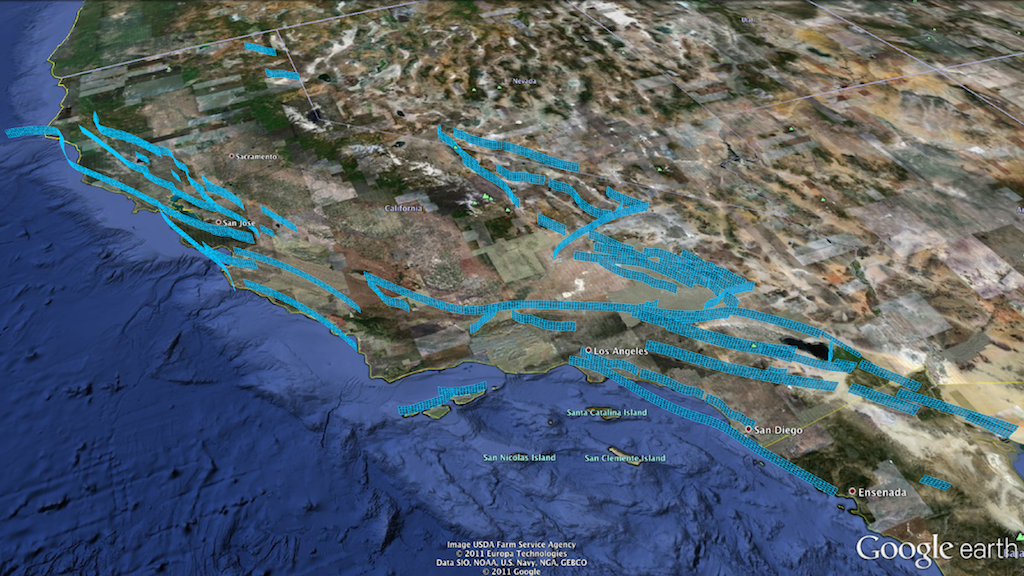
\includegraphics[width=1\textwidth]{graphics/UCERF2_faults_GoogleEarth}\caption{California fault system based on UCERF2, meshed into fault elements
and shown above ground.\label{fig:UCERF2_google_earth}}
\end{figure}



\subsection{Model Parameters and Initial Conditions}

Virtual Quake currently requires that the user specify the fault
geometry and the stress parameters on each element then run the simulation
based on this. These parameters are briefly described in the following
section, and explicit example fault models are constructed in chapter
\ref{cha:Cookbooks}.


\subsection{Setting Fault Parameters and Building a Fault Model\label{sec:define_mesh_faults}}

VQ treats a system of faults as multiple planar elements embedded
in a flat homogeneous halfspace. To run Virtual Quake the first
step is to define a fault system using a set of traces. Each trace
describes the points along a given fault closest to the surface as
well as fault characteristics at each trace point, such as long term
velocity, dip angle, rake angle, depth, etc. Details about the trace
file format are shown in Appendix \ref{sec:Trace-File-Format}.

In this example we look at the earthquake cycle and rupture mechanics
on a single 12 km by 12 km square fault. For simplicity, the trace of this
fault runs eastward for 12km starting from latitude/longitude (0,0)
and ending at latitude/longitude (0,0.1078). The definition of this
fault is in the file \texttt{examples/fault\_traces/single\_fault\_trace.txt}
and is also shown below.
\begin{verbatim}
# fault_id: ID number of the parent fault of this section
# num_points: Number of trace points comprising this section
# section_name: Name of the section
0 2 One_Element_Example
# latitude: Latitude of trace point
# longitude: Longitude of trace point
# altitude: Altitude of trace point (meters)
# depth_along_dip: Depth along dip (meters)
# slip_rate: Slip rate at trace point (centimeters/year)
# aseismic: Fraction of slip that is aseismic at point
# rake: Fault rake at trace point (degrees)
# dip: Fault dip at trace point (degrees)
# lame_mu: Lame's mu parameter at trace point (Pascals)
# lame_lambda: Lame's lambda parameter at trace point (Pascals)
0 0 0 12000 1 0 180 90 3e+10 3.2e+10
0 0.1078 0 12000 1 0 180 90 3e+10 3.2e+10
\end{verbatim}
The first non-comment line in this file gives the fault ID, number
of trace points, and section name. In this example, the section is named
``One\_Fault\_Example''. The section is associated with fault number 0.
This naming convention is used to allow a large fault to be split into multiple
sections for identification, but maintain the same physical properties as
a single full fault.

The remaining non-comment
lines give the fault characteristics at each trace point. This file
defines two trace points, the first at latitude/longitude (0,0) and
the second at (0, 0.1078), with both at altitude 0. At each point
the fault extends 12,000 meters down and has a slip rate of 1 cm/year
with 0 aseismicity. The fault is right lateral strike slip (rake of
180\textdegree{}, dip of 90\textdegree{}). The Lam� parameters of
$\mu=3e10$ and $\lambda=3.2e10$ indicate the material properties
of the fault interface.

Given this fault definition we can create a mesh which fits within
the fault dimensions. Each fault is meshed by specifying the fault
trace file in the format described above, and a fault element size.
Currently all fault elements in Virtual Quake are square though
future versions will allow triangular elements. Furthermore, all
elements of a single fault are meshed at the same resolution. This
means that if the meshing resolution is not a perfect multiple of
the trace length or depth at a given point, the meshed elements will
not completely cover the trace.

Figure \ref{fig:trace_mesh_example} shows this for an example fault
trace consisting of 4 trace points, where the fault trace is represented
by a dashed line and the meshed elements represented by red segments.
Figure \ref{fig:exact_trace_mesh} shows the meshed model on this
fault with elements that match the lengths between the trace points.
Because the distance between trace points is exactly a multiple of
the element size, the meshed elements exactly cover the fault trace.
Figure \ref{fig:offset_trace_mesh} shows the same fault trace with
smaller meshed elements. The first element follows the trace but the
second element deviates in order to fit the meshed element along the
trace. In practice, this discrepancy is usually not a big issue because
fault traces are not significantly non-linear. Also, as elements become
smaller relative to the distance between trace points this discrepancy
becomes smaller.

\begin{figure}
\subfloat[\label{fig:exact_trace_mesh}Using an element size that exactly aligns
with the trace, the generated elements will exactly follow the trace.]{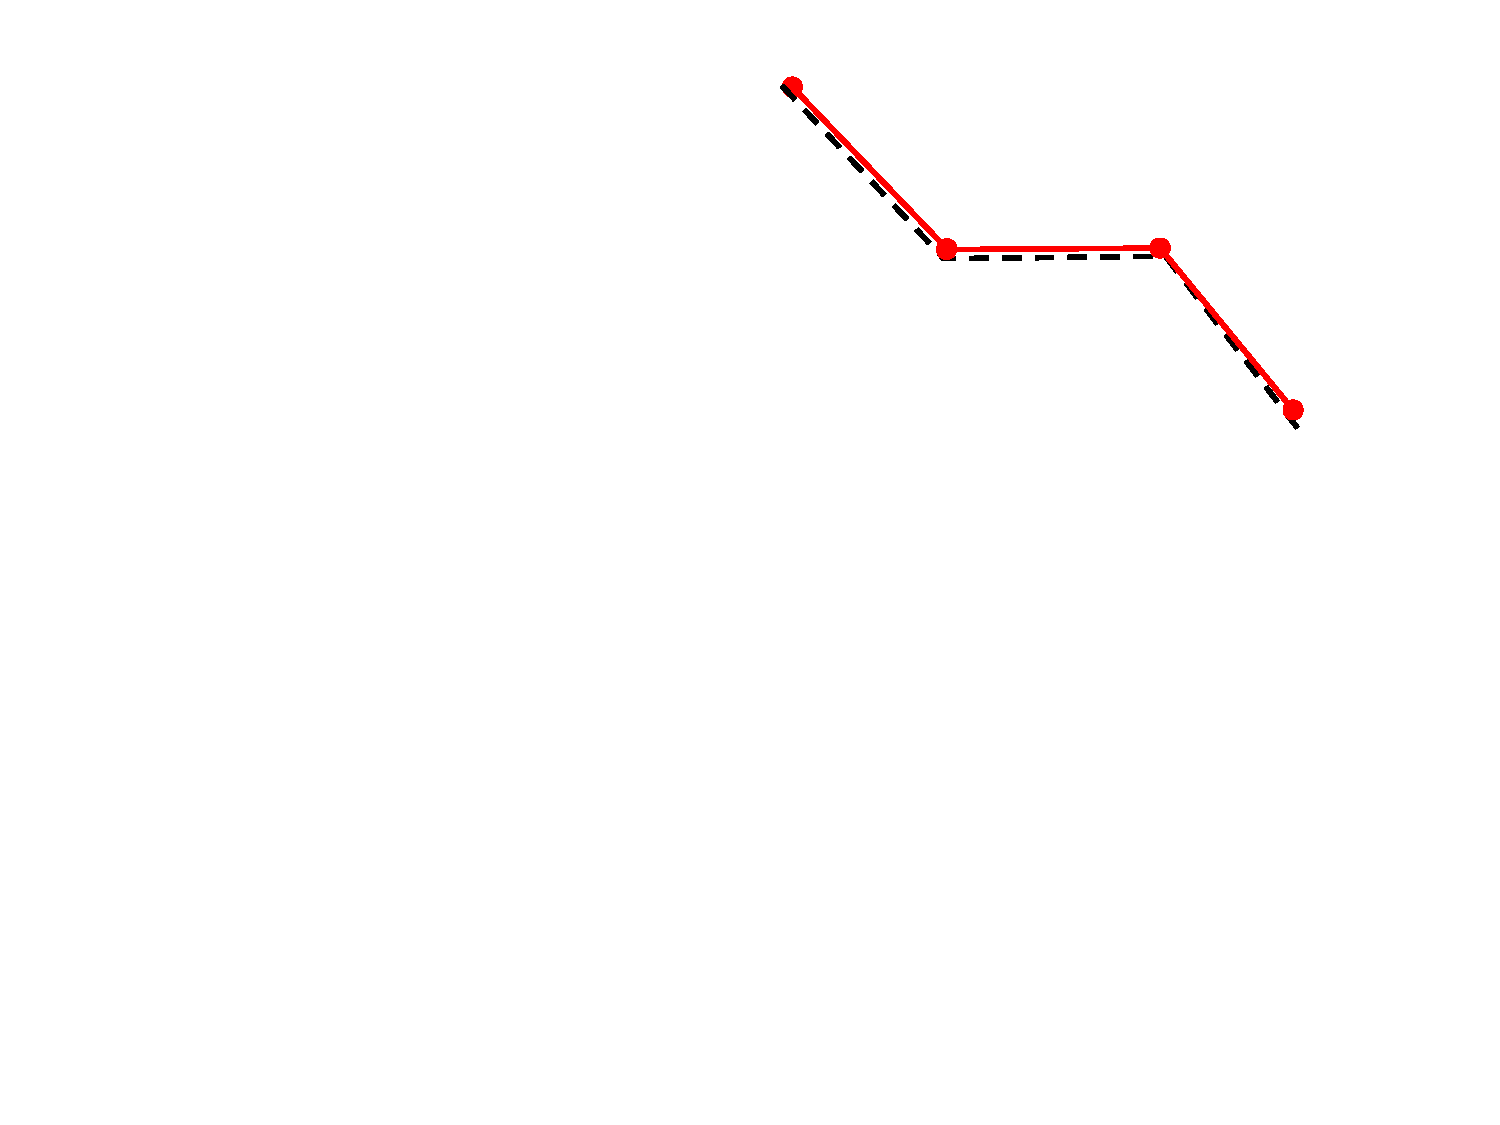
\includegraphics[width=0.48\textwidth]{graphics/FaultTrace3elem}}\hfill{}\subfloat[\label{fig:offset_trace_mesh}A slightly smaller element size results
in a mesh that does not exactly follow the trace.]{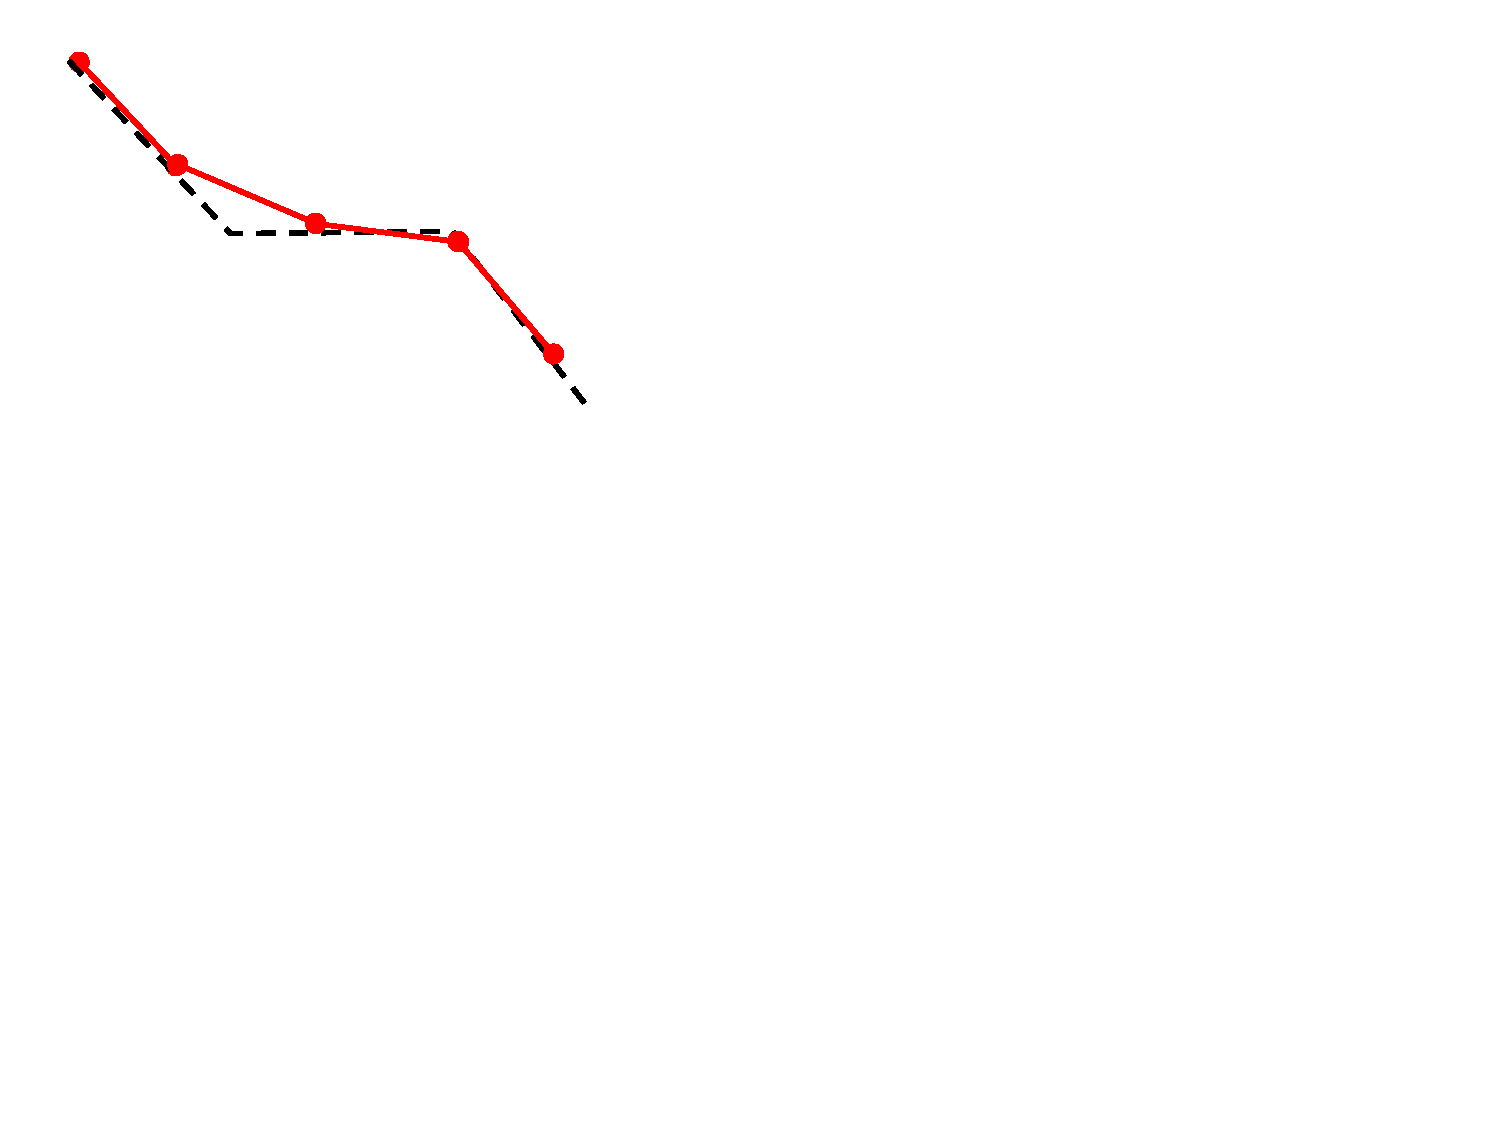
\includegraphics[width=0.48\textwidth]{graphics/FaultTrace4elem}

}

\caption{\label{fig:trace_mesh_example}An example of how element size will
affect the tracking of the mesh along a fault trace.}
\end{figure}


When creating a meshed element along a fault trace it is necessary
to assign characteristics to the element such as slip rate, aseismic
slip, rake, dip, and Lam� parameters. These are determined by linear
interpolation of the fault trace values at the midpoint of the meshed
element.

The use of linear interpolation for values between fault trace points
also means that if the meshed elements are larger than the distance
between fault trace points and there is significant variation between
trace point characteristics, then this variation may be lost during
the meshing process. In general it is recommended to use an element
size smaller than the smallest distance between fault trace points
unless there are memory or computing constraints. In the event that
the meshing process skips a trace point because of overly large element
size, a warning will be output during the meshing process. Appropriate element size is further
discussed in Section \ref{sec:element_size_discussion}. The meshing
program and related parameters are described in Section \ref{sec:building_faults}.

\begin{figure}
\subfloat[\label{fig:mesh6km}Example 12km x 12km fault meshed at 6km resolution
giving 2 x 2 = 4 total elements.]{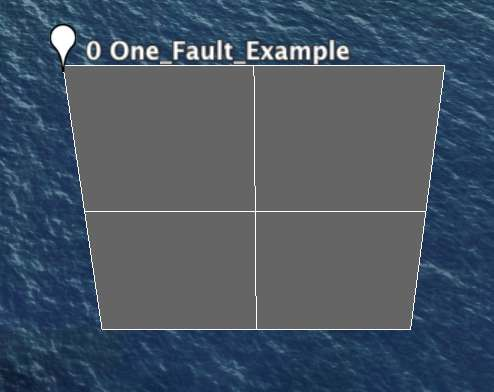
\includegraphics[height=5cm]{graphics/single_fault_6k}}\hfill{}\subfloat[\label{fig:mesh4km}Example 12km x 12km fault meshed at 4km element
resolution giving 3 x 3 = 9 total elements.]{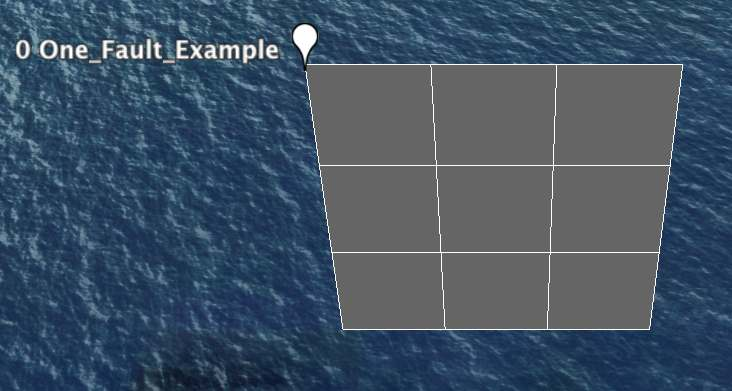
\includegraphics[height=5cm]{graphics/single_fault_4k}

}

\caption{\label{fig:meshing-example}A demonstration of meshing with different
resolutions.}
\end{figure}


Figure \ref{fig:meshing-example} shows the result of meshing the
One\_Fault\_Example trace with different element resolutions. Figures
\ref{fig:mesh6km} and \ref{fig:mesh4km} show the KML output of the
program in Google Earth. Since the fault is defined to
start at latitude/longitude (0,0) it will appear in the middle of
the Atlantic ocean. In output KML files the depth is reversed so faults
are visible above the surface. When performing simulations with realistic
fault systems it is better to use actual fault latitude/longitude rather than centering the faults on (0,0)
in the traces to help visualize the simulation results.


\section{Element Stress Interactions}

Unlike actual fault systems where the fault geometry is dynamic over
long time periods, Virtual Quake simplifies calculations assuming
a geometrically static fault system. In this way Virtual Quake
is intended to explore seismicity in fault systems as they appear
today rather than attempting to model their long term evolution. Back
slip is used to model the effects of stress buildup and release along
elements approximating the fault plane. In a back slip model, the
equilibrium and initial positions of an element are the same, thus
when an element fails it moves towards the original position and the
fault system geometry remains static.


\subsection{Green's Functions}

Interactions between fault elements depend on the relative position
and orientation of each element, and are calculated using stress Green's
functions at the start of the simulation. The change in stress at
a location $x$ due to movement of all elements is given by \cite{Rundle2006vc}:

\begin{equation}
\sigma_{ij}(x,t)=\int dx_{k}^{'}T_{ij}^{kl}(x-x')s_{l}(x',t)\label{eq:stress_field}
\end{equation}


where $s_{l}(x',t)$ is the three-dimensional slip density of element
$l$, $T_{ij}^{kl}(x-x')$ is the Green's function tensor, and $l$
goes over all elements. In Virtual Quake this field is evaluated
only at the center of elements and slip is assumed to be uniform across
the surface of an element and along the element rake angle defined
in the model. Under these conditions equation \ref{eq:stress_field}
simplifies to:

\begin{equation}
\sigma_{ij}^{A}(t)=\sum T_{ij}^{AB}s_{B}(t)\label{eq:simple_stress_field}
\end{equation}


where B runs over all elements. Finally, since Virtual Quake
only uses the shear stress along the element rake vector and normal
stress perpendicular to the element, the tensor $T_{ij}^{AB}$ reduces
to $T_{s}$ for shear stresses and $T_{n}$ for normal stresses. This
means the shear and normal stresses on an element in Virtual Quake
are calculated as:

\begin{equation}
\sigma_{s}^{A}(t)=\sum T_{s}^{AB}s_{B}(t)\label{eq:shear_stress_sum}
\end{equation}


\begin{equation}
\sigma_{n}^{A}(t)=\sum T_{n}^{AB}s_{B}(t)\label{eq:norm_stress_sum}
\end{equation}


Thus, for a fault model with $N$ elements Virtual Quake requires
two $N\times N$ element matrices to represent all interactions. These
are also referred to as the Green's function matrices. The actual
values for the matrix entries are calculated using Okada's half-space
deformation equations \cite{Okada01041992}. Figure \vref{fig:okada_stress_field}
shows the stress field for a single vertical strike-slip fault element. 


\subsection{Event Transition Time}

Virtual Quake uses a combined static-dynamic friction law to
calculate element failures. This law is based on the Coulomb failure
function (CFF):

\begin{equation}
CFF^{A}(t)=\sigma_{s}^{A}(t)-\mu_{s}^{A}\sigma_{n}^{A}(t)\label{eq:cff_function}
\end{equation}


where $\mu_{s}^{A}$ is the static coefficient of friction on element
$A$ based on model element strengths. During long term stress accumulation,
an element is defined to fail at time $t_{f}$ when $CFF^{A}(t_{f})=0$,
which is referred to as static failure. At this point the simulation
changes to the rupture event model described below.

Given the change in stress over time it is relatively straightforward
to calculate the time to failure for an element. Since effective long
term slip rates during stress accumulation are assumed to be constant
the change in CFF over time is governed by the equation:

\begin{equation}
\frac{dCFF^{A}}{dt}=(\sigma_{s}^{A}-\mu_{s}^{A}\sigma_{n}^{A})+\alpha T_{\alpha}^{A}\label{eq:cff_change}
\end{equation}


where $\alpha$ represents the fraction of fault slip that is aseismic
and $T_{\alpha}^{A}=\frac{CFF^{A}T^{AA}}{recurrence}$ represents the instantaneous
change in CFF due to aseismic slip. Aseismic slip on an element transmits
stress to other elements but not on the element itself. 

Knowing the relationship between slip and stress (equations \ref{eq:shear_stress_sum}
and \ref{eq:norm_stress_sum}), it is not necessary to evolve the system
time step by time step. Rather, the simulation time is advanced directly
to the point at which the next element fails. Equations \ref{eq:cff_function}
and \ref{eq:cff_change} allow us to analytically solve for the time
when the next element will fail.


\section{Rupture Event Model\label{sec:Event_Model}}

A rupture event in VQ is comprised of multiple sweeps.  During each sweep one or more elements fail and one or more elements slip.  The sweeps continue as long as there are elements that fail - once no more elements fail the event is complete.

Rupture propagation consists of two internal phases - rupture/slip caused by static or dynamic failure and slip caused by the stress influence of other elements.  The first phase involves elements rupturing and slipping due to static stress failure (CFF = 0) or dynamic failure (Equation \ref{eq:dynamic_trigger}).  The second phase involves ruptured elements continuing to slip due to the changing stress influence of other elements.  Each of these phases are described below.

During rupture propagation elements are either in a ruptured or non-ruptured state.  Elements move from the non-ruptured to ruptured state either by static or dynamic failure.  Elements move from ruptured to non-ruptured only when the event is complete.  Static failure occurs when $CFF \geq 0$. To better model rupture propagation dynamic
failure is also allowed during rupture events. Dynamic failure allows
elements on the same fault and physically nearby to failed elements
to in turn fail at a lower stress level than the static failure
criterion. This dynamic failure is based on the increase in stress
during the rupture event. Dynamic failure is caused when there is a significant change in CFF during the event, satisfying:

\begin{equation}
\frac{CFF_{init}-CFF_{final}}{CFF_{init}}>\eta\label{eq:dynamic_trigger}
\end{equation}

where $\eta$ is a user defined dynamic triggering parameter either
for the whole system or uniquely defined for each element. This parameter
approximates the stress intensity factor at the tip of a propagating
rupture.

The initial element rupture during an event is always caused by static failure.
During rupture propagation the first element to fail slips back towards
the equilibrium position. The amount of slip during the initial failure,
$\Delta s$, is related to the stress drop defined for the element
in the model, $\Delta\sigma$, by \cite{Rundle2006vc}:

\begin{eqnarray}
\Delta s & = & \frac{1}{K_{L}}(\Delta\sigma-CFF).\label{eq:sst_two}
\end{eqnarray}

where $K_{L}$ is the element's stiffness or self-stress defined as
$K_{L}=T_{s}^{AA}-\mu_{s}^{A}T_{n}^{AA}$.  Once an element has ruptured due to static or dynamic failure it will no longer slip in the event due to these failures.  However, ruptured elements may slip further due to the movement of other elements.

During each rupture sweep, ruptured elements may slip further due to movement on other elements.  The amount of slip on a failed element is related to the movement of other elements through the Green's function.  A simplistic approach to determining this is to calculate the slip on all other elements when a given element moves.  However, this is highly inefficient because the slip on a given element will in turn cause slip on all ruptured elements, which will cause slip on all ruptured elements, and so on forever.  Instead, the system is described using a set of linear equations relating the slip of each element to the stress on all other elements in the final state of a given sweep.

This relationship between element slips during a sweep is determined for each ruptured element $A$ as:

\begin{eqnarray}
0 = \sum (T_s^{AB} - \mu_s^B T_n^{AB}) s_B
\end{eqnarray}

Since non-ruptured blocks do not change their slip, they are excluded from the system. This system is then solved using Gaussian elimination.
Once the slip is calculated for all ruptured elements, a new stress state for the entire system is calculated using Equations \ref{eq:shear_stress_sum} and \ref{eq:norm_stress_sum}.  The rupture process is repeated by again checking the static/dynamic failure until no more elements have failed.

\begin{figure}
\subfloat[CFF vs. time for a series of stress buildup and rupture events.]{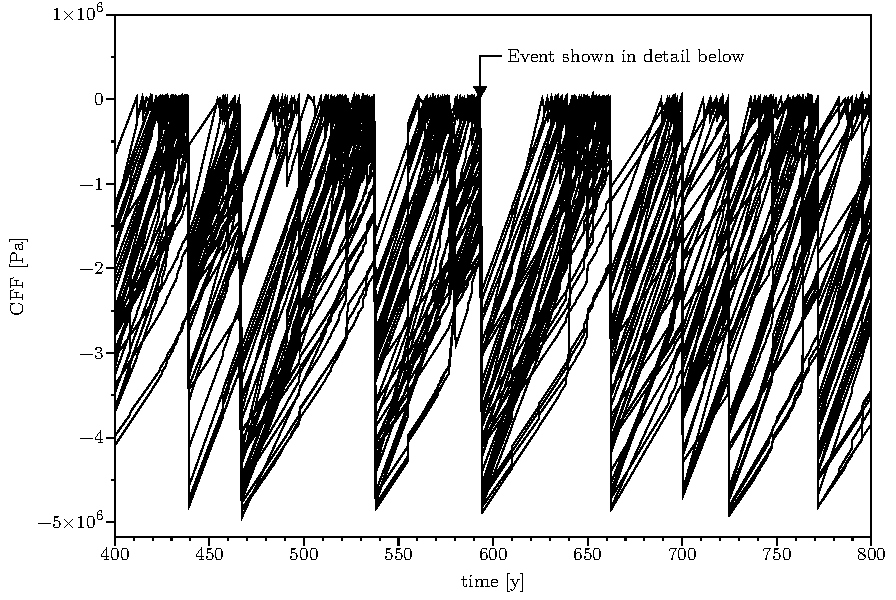
\includegraphics[width=0.48\textwidth]{graphics/CFF_1}

}\hfill{}\subfloat[CFF vs. sweeps for the event at t=593]{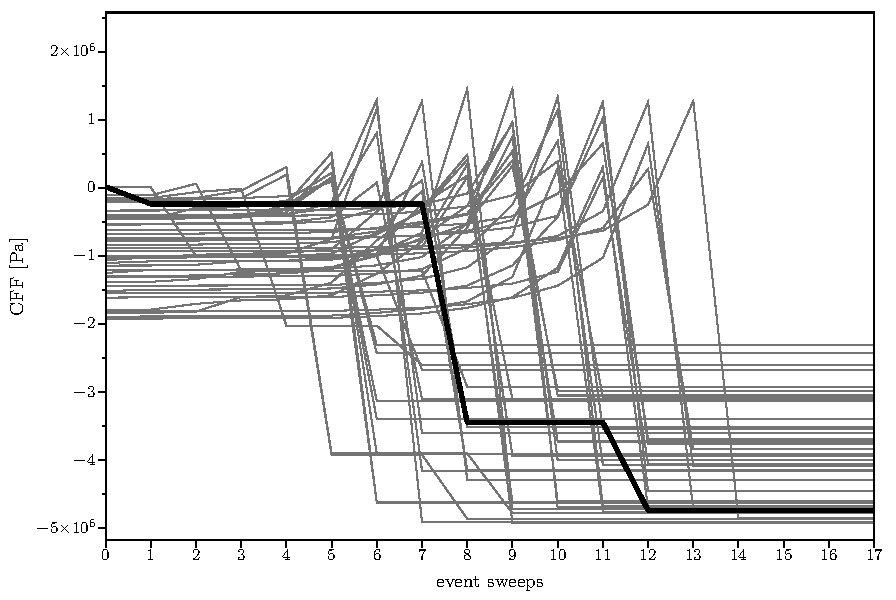
\includegraphics[width=0.48\textwidth]{graphics/CFF_2}

}\caption{Top: The CFF for each of the 48 elements comprising the Parkfield
section of the San Andreas fault. Drops in CFF correspond to stress
release in events, with larger events consisting of many elements
releasing stress. Bottom: detail of rupture sweeps from the event
at t=593. The trigger element is shown bold. Note that elements may
experience multiple failures, such as the trigger element failing
during sweeps 0, 7, and 11.\label{fig:cff_example_history}}
\end{figure}


Examples of stress accumulation and release over multiple phases of
long term stress accumulation and rupture events are shown in Figure
\ref{fig:cff_example_history}. The first figure shows how a single
element failure leads to a rupture spanning multiple elements and
how stress builds up and releases in cycles over time. The second
figure shows how elements may fail multiple times during different
sweeps in an event, but do not accumulate additional stress after
failing.

\section{Simulation Flow}

\begin{figure}[th]
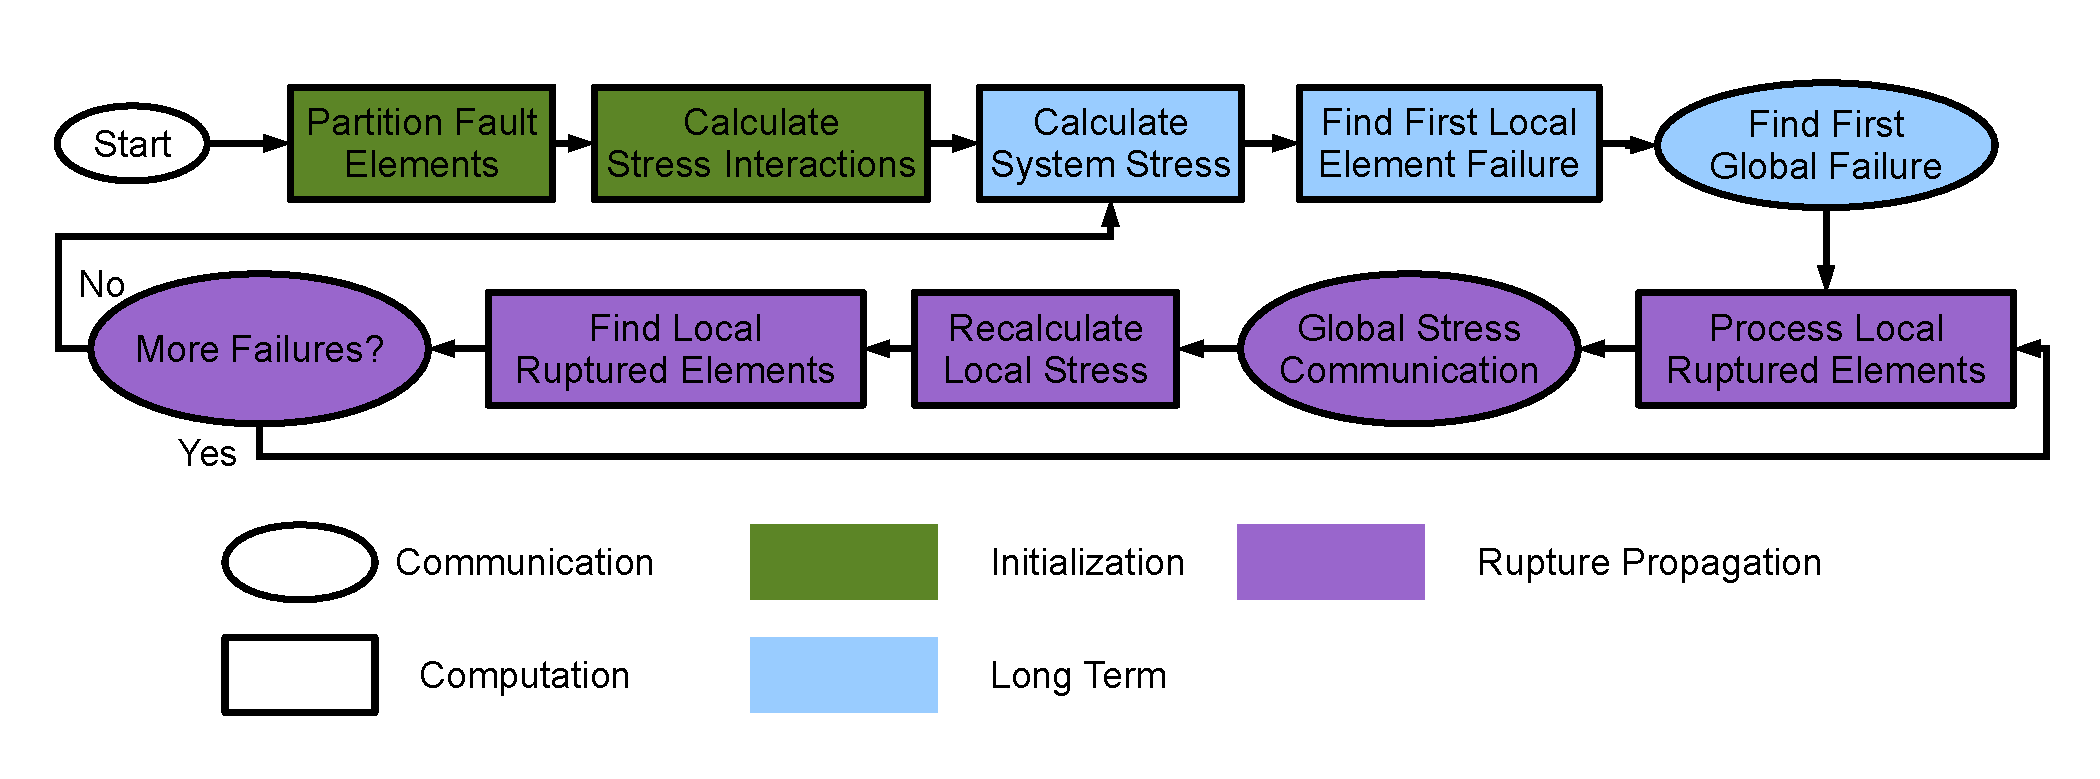
\includegraphics[width=0.99\textwidth]{graphics/VQFlow}\caption{Simulation flow of Virtual Quake.\label{fig:simulation_flow}}
\end{figure}
Figure \ref{fig:simulation_flow} shows the flow of simulation in
Virtual Quake. The simulation begins by reading in a set of faults
and converting them to the internal data structures. When running
a parallel simulation, these are partitioned over multiple processes
to ensure that each process is responsible for roughly an equal number
of elements and that elements on the same processor are on the same
fault or geographically close to each other. Next, each processor
calculates the stress Green's functions on the local elements for
all other elements in the model or loads precomputed Green's functions
from a file. This comprises the initialization phase of the simulation
shown in green in Figure \ref{fig:simulation_flow}.

The core of the simulation consists of repeated cycling between two
phases until the end of the simulation time. The first phase, shown
in blue, calculates the long term stress buildup and time to first
element failure in the system based on Equation \ref{eq:cff_function}.
In parallel simulations this time is calculated locally on each process
then reduced to a global time to failure.

The second phase is the rupture propagation phase, shown in purple
in Figure \ref{fig:simulation_flow}. Virtual Quake uses a cellular
automata style approach to modeling rupture propagation. The rupture
phase does not involve time domain solutions to differential equations,
but rather iterative calculations of stress and element failure to
approximate a rupture propagating through the fault system.


\section{QuakeLib Tour \label{sec:quakelib_tour}}

As mentioned in Section \ref{sec:About_quakelib}, the QuakeLib library
provides tools and a Python interface to develop earthquake simulations,
read/write EqSim or VQ format files for geometry, friction, initial conditions
and events, and calculate Okada's functions for arbitrary fault geometries. 
QuakeLib can be compiled and used independently from Virtual Quake.
To only compile QuakeLib, follow the install instructions in section
\ref{sec:Install} but from the quakelib subdirectory.

This chapter provides a brief visual tour of a few analytical utilities
in QuakeLib and to illustrate its capacity as the computational backbone
for impressive and informative visualizations. The script that generates
these plots is vq/pyvq/pyvq.py, and a tutorial for generating plots like these
is given in section \ref{sec:pyvq}.

\subsection{Conventions}

The QuakeLib functions act on single fault elements, and compute various
dynamic quantities like the stress tensor, surface deformation field,
and gravity anomalies. These functions take fault parameter values
following Okada's convention \cite{Okada01041992}. Figure \ref{fig:okada_convention}
shows Okada's convention for fault plane elements in an elastic halfspace
$z \leq 0$. The two Lam� parameters ($\lambda$,$\mu$) that describe
the fault element's elasticity are also required. These parameters
and their units are described in detail in Appendix \ref{sec:Trace-File-Format}.

\begin{center}
\begin{figure}
\begin{centering}
\begin{minipage}[t]{0.45\columnwidth}%
\begin{center}
\subfloat{\noindent \centering{}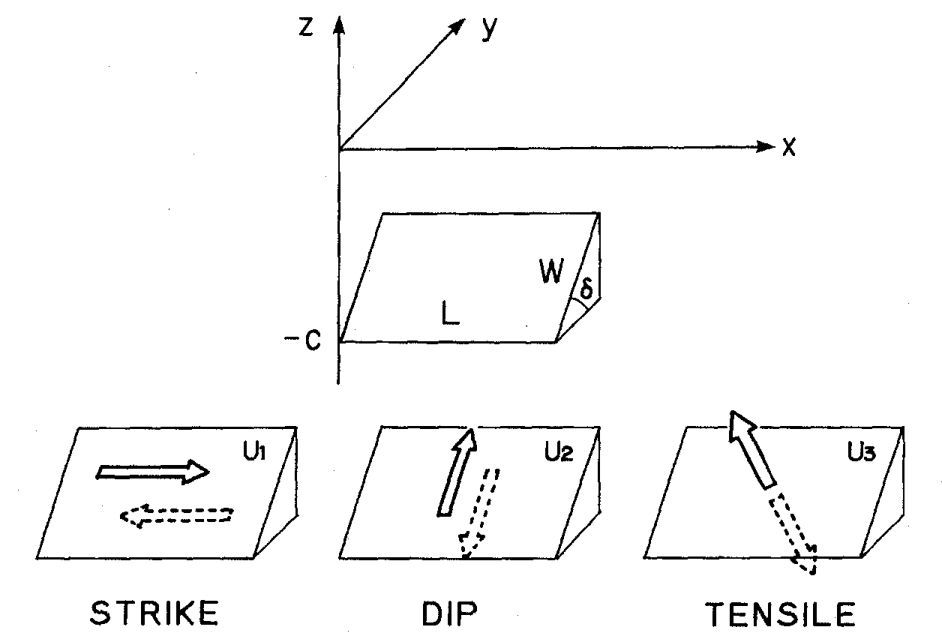
\includegraphics[width=1\textwidth]{graphics/Okada_Fault_Convention}}
\par\end{center}%
\end{minipage}\hspace{1cm}%
\begin{minipage}[t]{0.35\columnwidth}%
\begin{center}
\subfloat{\raggedright{}%
\begin{tabular}{|c|c|}
\hline 
\textsf{\textbf{\small{Parameter}}} & \textsf{\textbf{\small{Description}}}\tabularnewline
\hline 
\hline 
\textsf{\small{L, W}} & \textsf{\small{Fault length, down-dip width}}\tabularnewline
\hline 
\textsf{\small{$\delta$}} & \textsf{\small{Dip angle}}\tabularnewline
\hline 
\textsf{\small{C}} & \textsf{\small{Fault plane depth}}\tabularnewline
\hline 
\textsf{\small{U1}} & \textsf{\small{Slip unit vector for strike-slip}}\tabularnewline
\hline 
\textsf{\small{U2}} & \textsf{\small{Slip unit vector for dip-slip}}\tabularnewline
 & \textsf{\small{(U2\textgreater{}0 thrust; U2\textless{}0 normal)}}\tabularnewline
\hline 
\textsf{\small{U3}} & \textsf{\small{Slip unit vector for tensile}}\tabularnewline
\hline 
\textsf{\small{z}} & \textsf{\small{Distance below surface}}\tabularnewline
\hline 
\textsf{\small{x/y}} & \textsf{\small{Distance on surface}}\tabularnewline
\hline 
\end{tabular}}
\par\end{center}%
\end{minipage}\hspace{1.5cm}
\par\end{centering}

\caption{QuakeLib defines each fault element with parameters following Okada's
convention.\label{fig:okada_convention}}
\end{figure}

\par\end{center}


\subsection{Single Element Examples}

The following example plots provide a brief window into QuakeLib's
analytical tools applied to single fault elements.


\subsubsection{Stress Field\label{sec:quakelib_stress_field}}

The stress field Green's function is defined in quakelib/src/QuakeLibOkada.cpp
as \textbf{calc\_stress\_tensor. }This function computes the stress
tensor at an arbitrary location in the elastic halfspace around the fault plane.
Examples of the shear stress field -- equation \ref{eq:shear_stress_sum}
-- computed by QuakeLib for a single vertical ($\delta = 90^{\circ}$)
strike slip fault element are shown in Figure \ref{fig:okada_stress_field}.

\begin{center}
\begin{figure}
\begin{centering}
\subfloat[Front view]{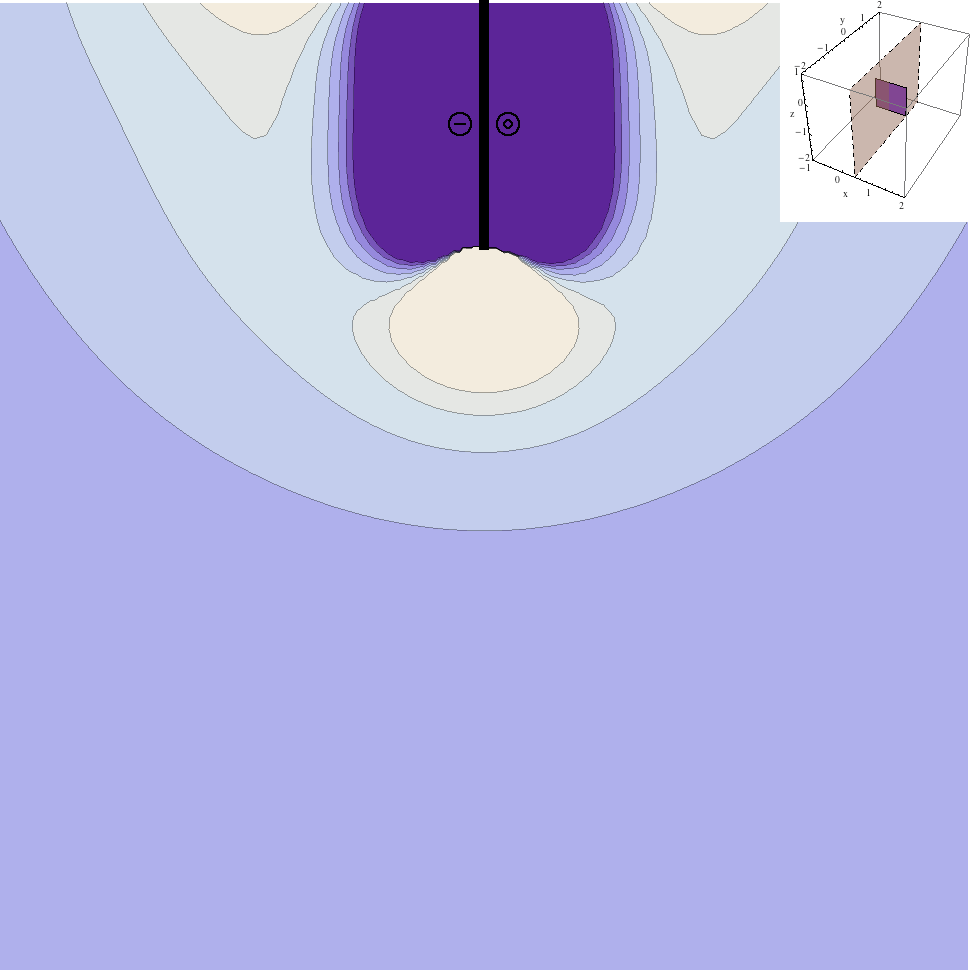
\includegraphics[width=0.42\textwidth]{graphics/sigma_s_front}

}\hfill{}\subfloat[Top view]{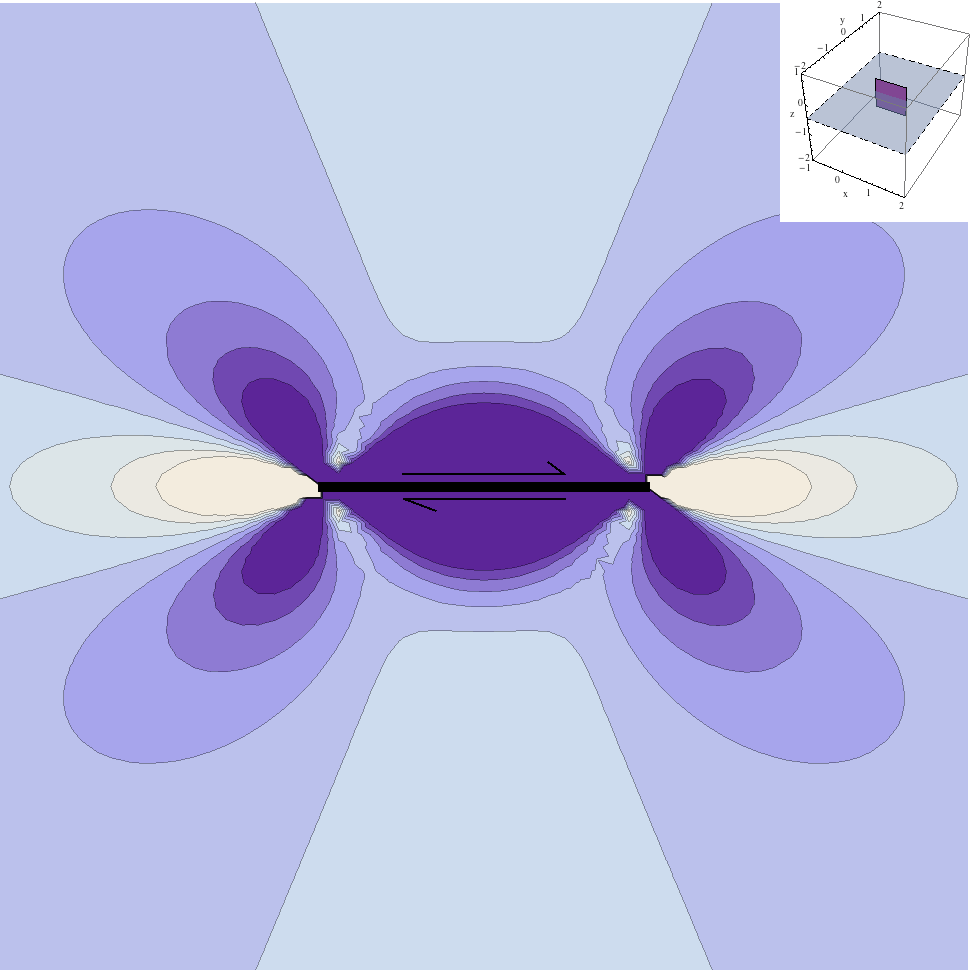
\includegraphics[width=0.42\textwidth]{graphics/sigma_s_top}}
\par\end{centering}

\caption{The shear stress field $\sigma_{xy}$ (tan $\sigma_{xy}>0$, blue
$\sigma_{xy}<0$) created by horizontal backslip, viewed from the
front and top of an element. The direction of backslip is indicated
by the arrows.\label{fig:okada_stress_field}}
\end{figure}

\par\end{center}


\subsubsection{Displacement Field}

The Green's function is defined in quakelib/src/QuakeLibOkada.cpp
as\textbf{ calc\_displacement\_vector.} This function computes the
co-seismic displacement vector for an arbitrary location in the elastic halfspace
around the fault plane. Figure \ref{fig:single_element_displacements} shows
displacement fields for faults of different dips as calculated by this function.
In this figure the parameters for each fault element
are L = 10km, W = 10km, slip = 5m, and the horizontal/vertical axes
measure distance on the surface of the halfspace in km. The fault
plane depth values (C) are 10km for strike-slip, 11km for normal,
and 6km for thrust. The view is from above the fault plane looking
straight down at the surface, and the thick black lines are the projections
of the buried fault plane onto the surface of the halfspace.

\begin{center}
\begin{figure}
\begin{centering}
\begin{minipage}[t]{0.32\columnwidth}%
\begin{center}
\subfloat{\noindent \centering{}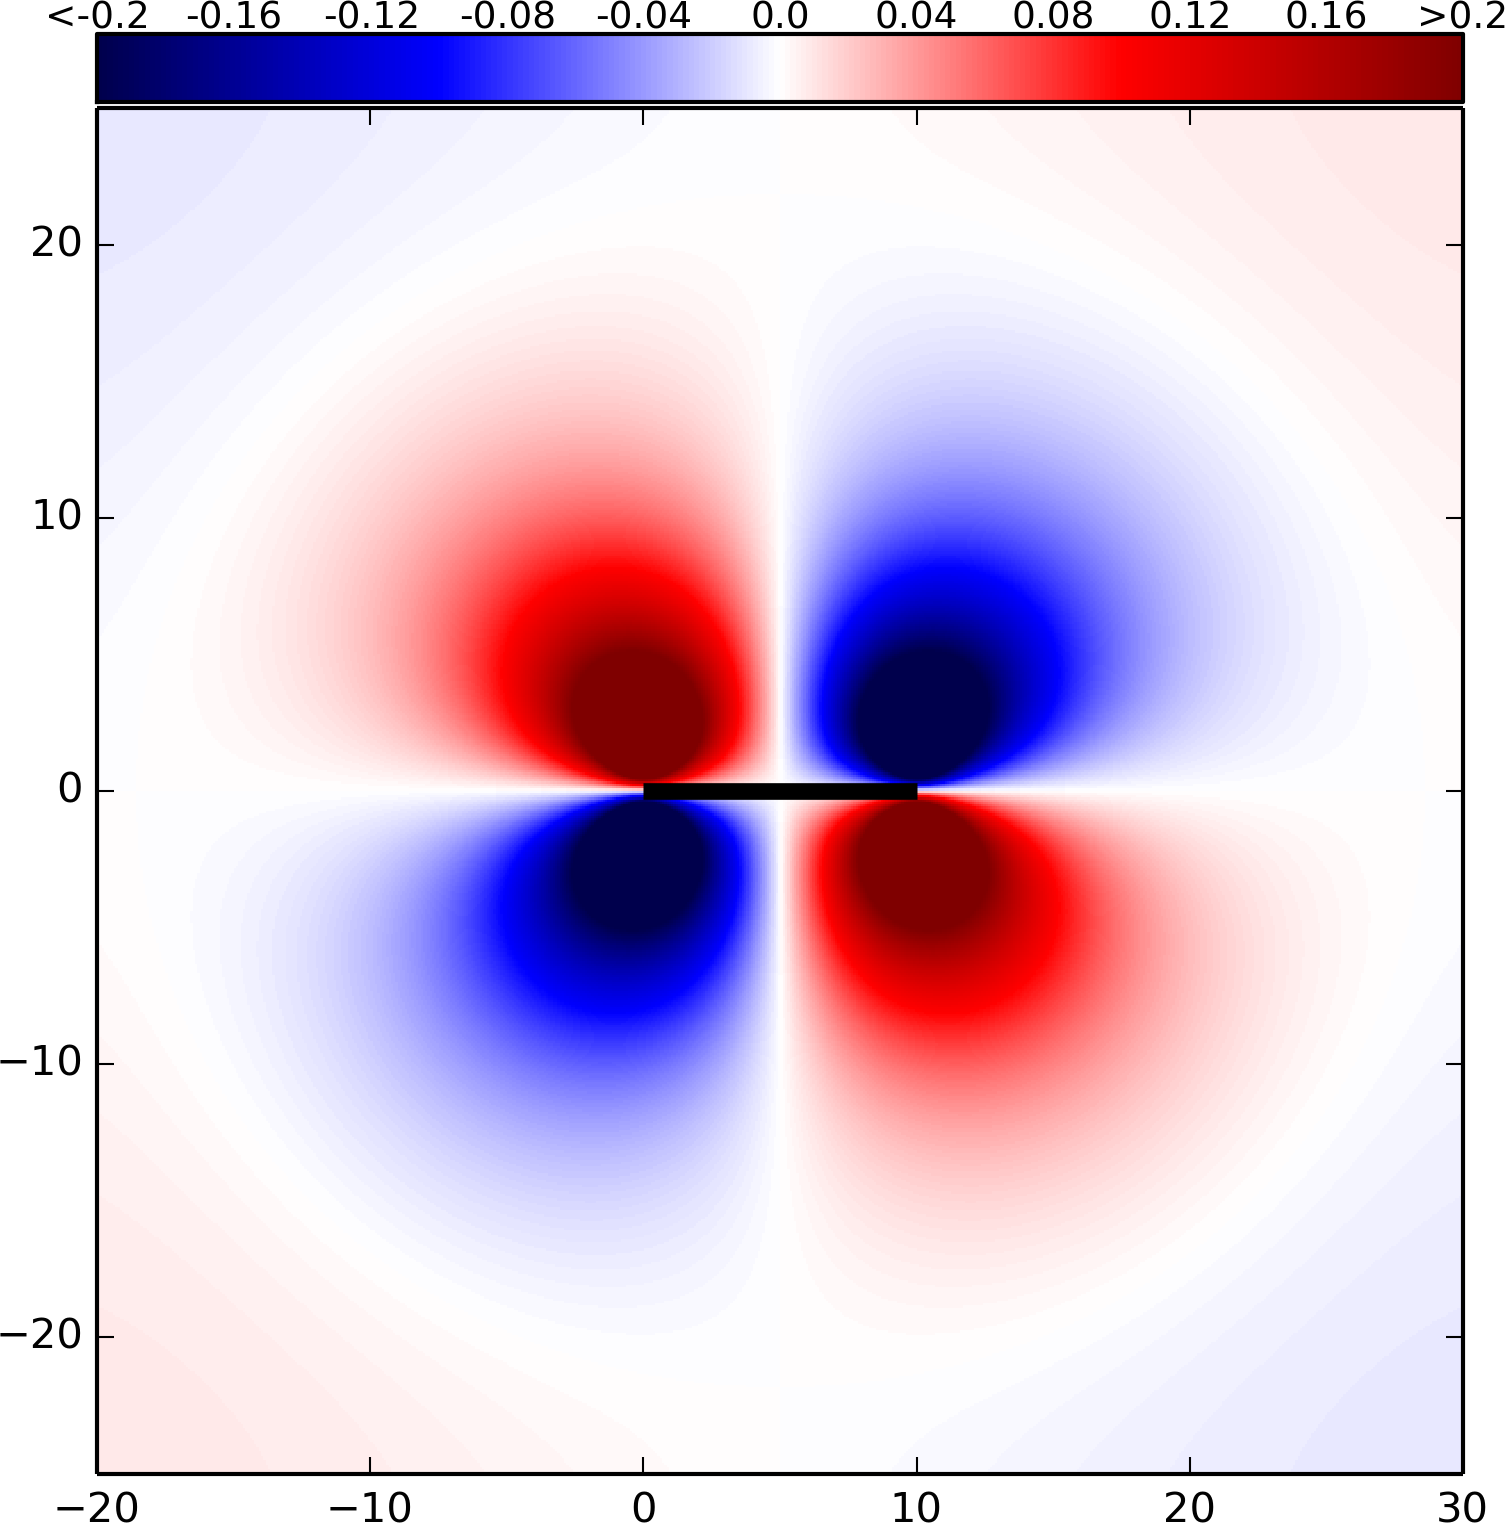
\includegraphics[width=1\textwidth]{graphics/dz_strikeslip5_dip90_L10k_W10k_c11k_docs_trim}}
\par\end{center}%
\end{minipage}\hfill{}%
\begin{minipage}[t]{0.32\columnwidth}%
\begin{center}
\subfloat{\noindent \centering{}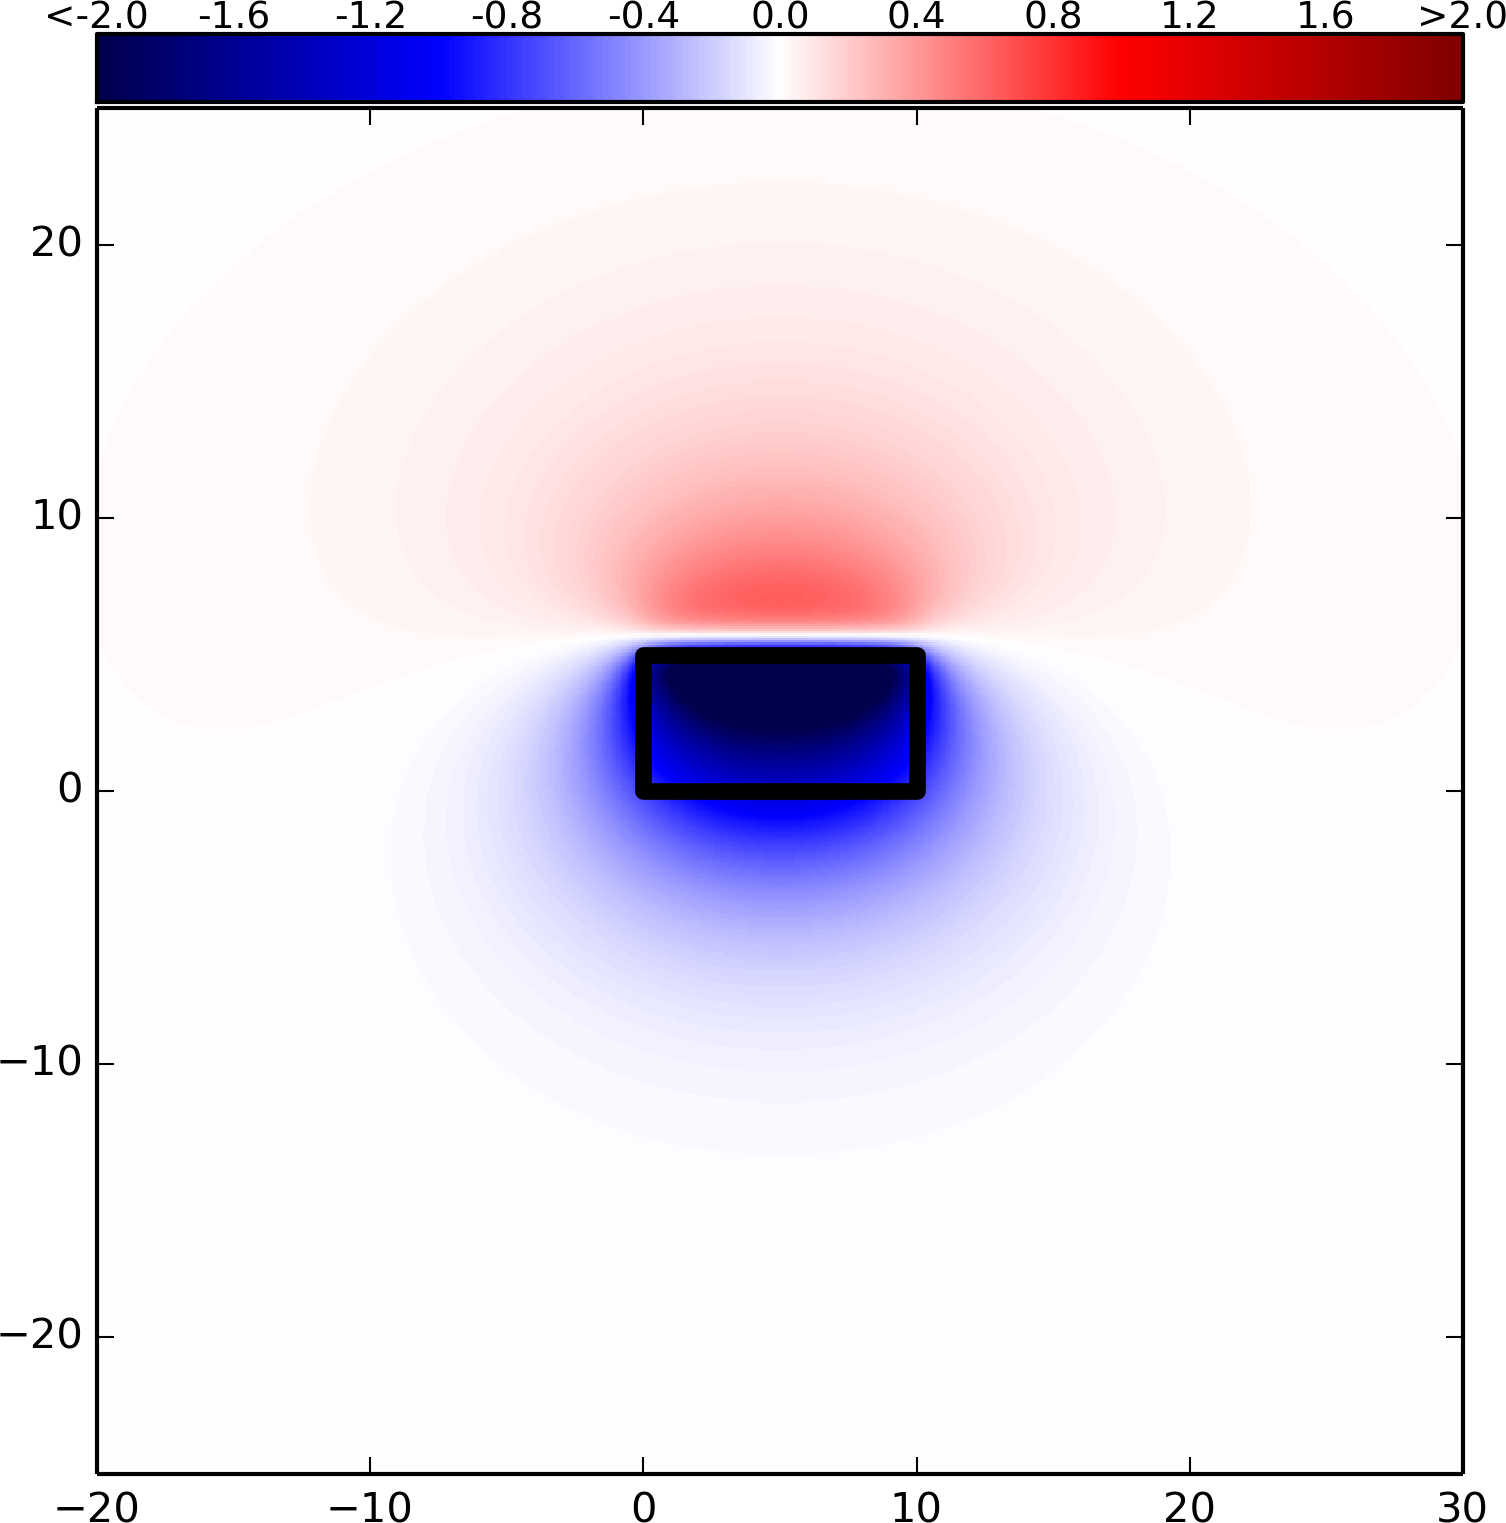
\includegraphics[width=1\textwidth]{graphics/dz_normal5_dip60_L10k_W10k_c10k_docs_trim}}
\par\end{center}%
\end{minipage}\hfill{}%
\begin{minipage}[t]{0.32\columnwidth}%
\begin{center}
\subfloat{\noindent \centering{}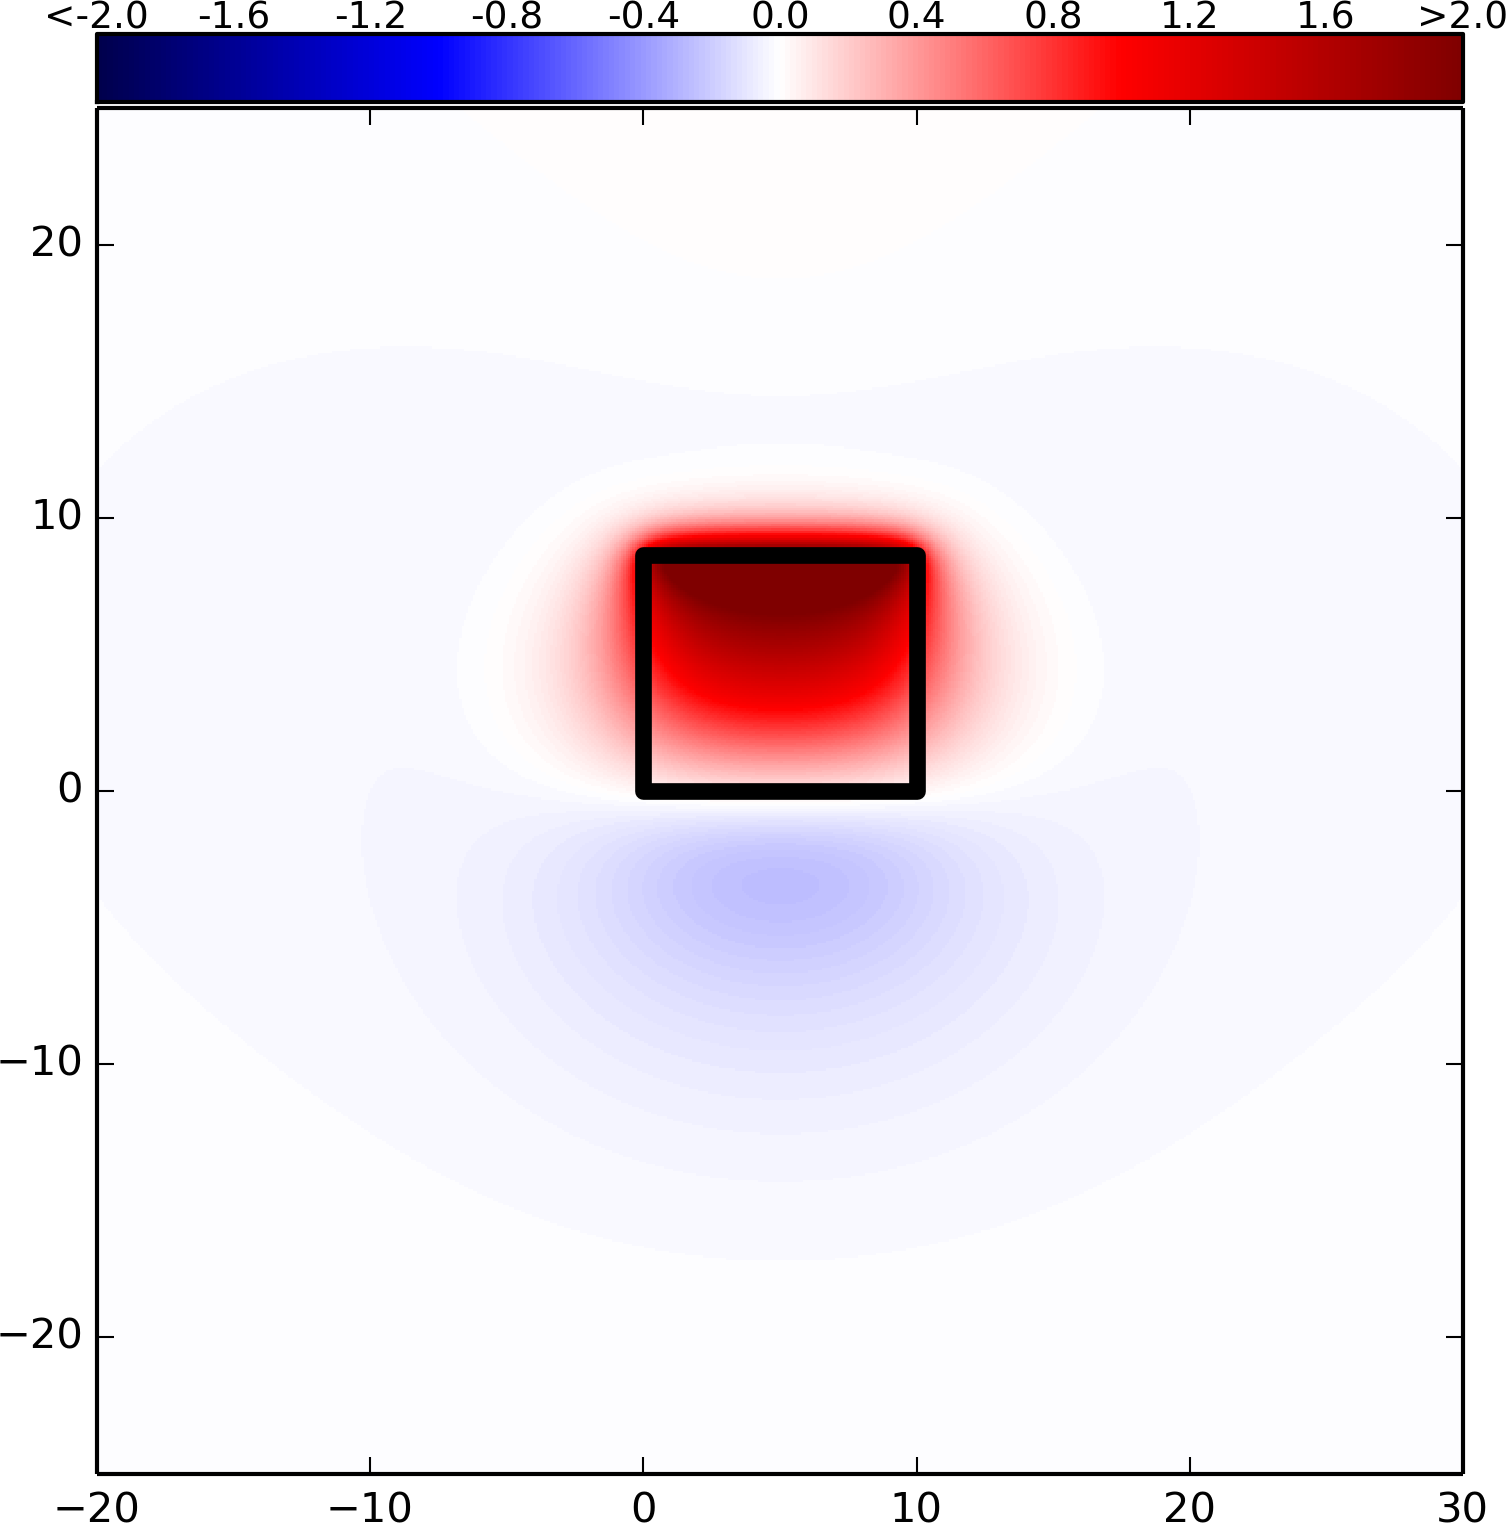
\includegraphics[width=1\textwidth]{graphics/dz_thrust5_dip30_L10k_W10k_c6k_docs_trim}}
\par\end{center}%
\end{minipage}
\par\end{centering}

\caption{Vertical displacement at the surface for buried fault elements, depth
to top of each fault plane is 1km, colorbar units are meters. \textbf{Left:}
strike-slip $\delta = 90^{\circ}$. \textbf{Center:} normal $\delta = 60^{\circ}$.
\textbf{Right:} thrust $\delta = 30^{\circ}$.\label{fig:single_element_displacements}}
\end{figure}

\par\end{center}


\subsubsection{Gravity Field Anomalies}

The gravity Green's function is defined in quakelib/src/QuakeLibOkada.cpp
as \textbf{calc}\_\textbf{dg. }This function computes the gravity
anomalies at an arbitrary surface location on the elastic halfspace around the fault
plane. This is the total gravity field anomaly Green's functions,
which includes contributions from subsurface density changes (dilatational)
and from surface displacement (free-air). Examples of the gravity
anomaly field for single fault elements is given in Figure \ref{fig:single_element_gravity_changes}.
The fault parameters are the same as above.


\begin{center}
\begin{figure}
\begin{minipage}[t]{0.32\columnwidth}%
\begin{center}
\subfloat{\noindent \centering{}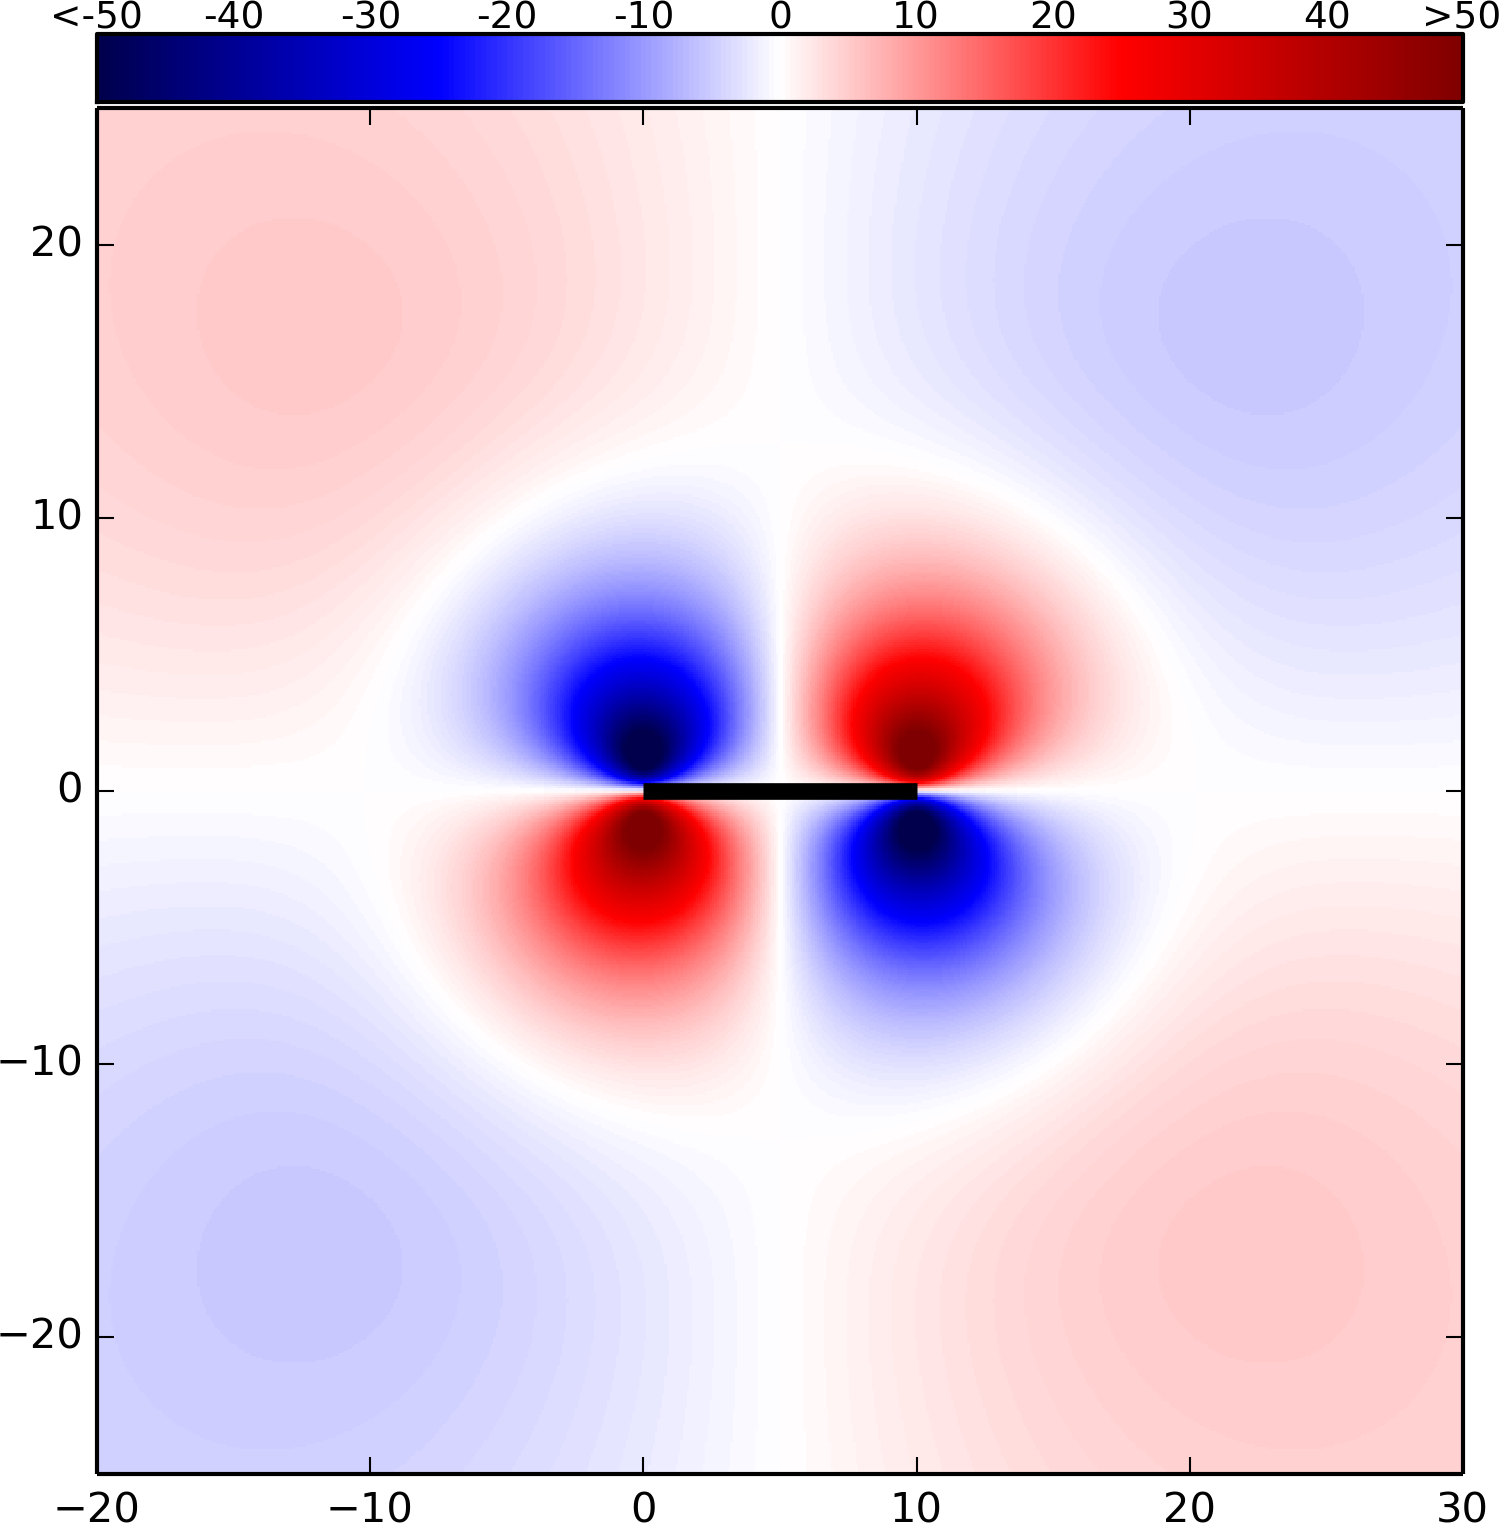
\includegraphics[width=1\textwidth]{graphics/dg_strikeslip5_dip90_L10k_W10k_c11k_docs_trim}}
\par\end{center}%
\end{minipage}\hfill{}%
\begin{minipage}[t]{0.32\columnwidth}%
\begin{center}
\subfloat{\noindent \centering{}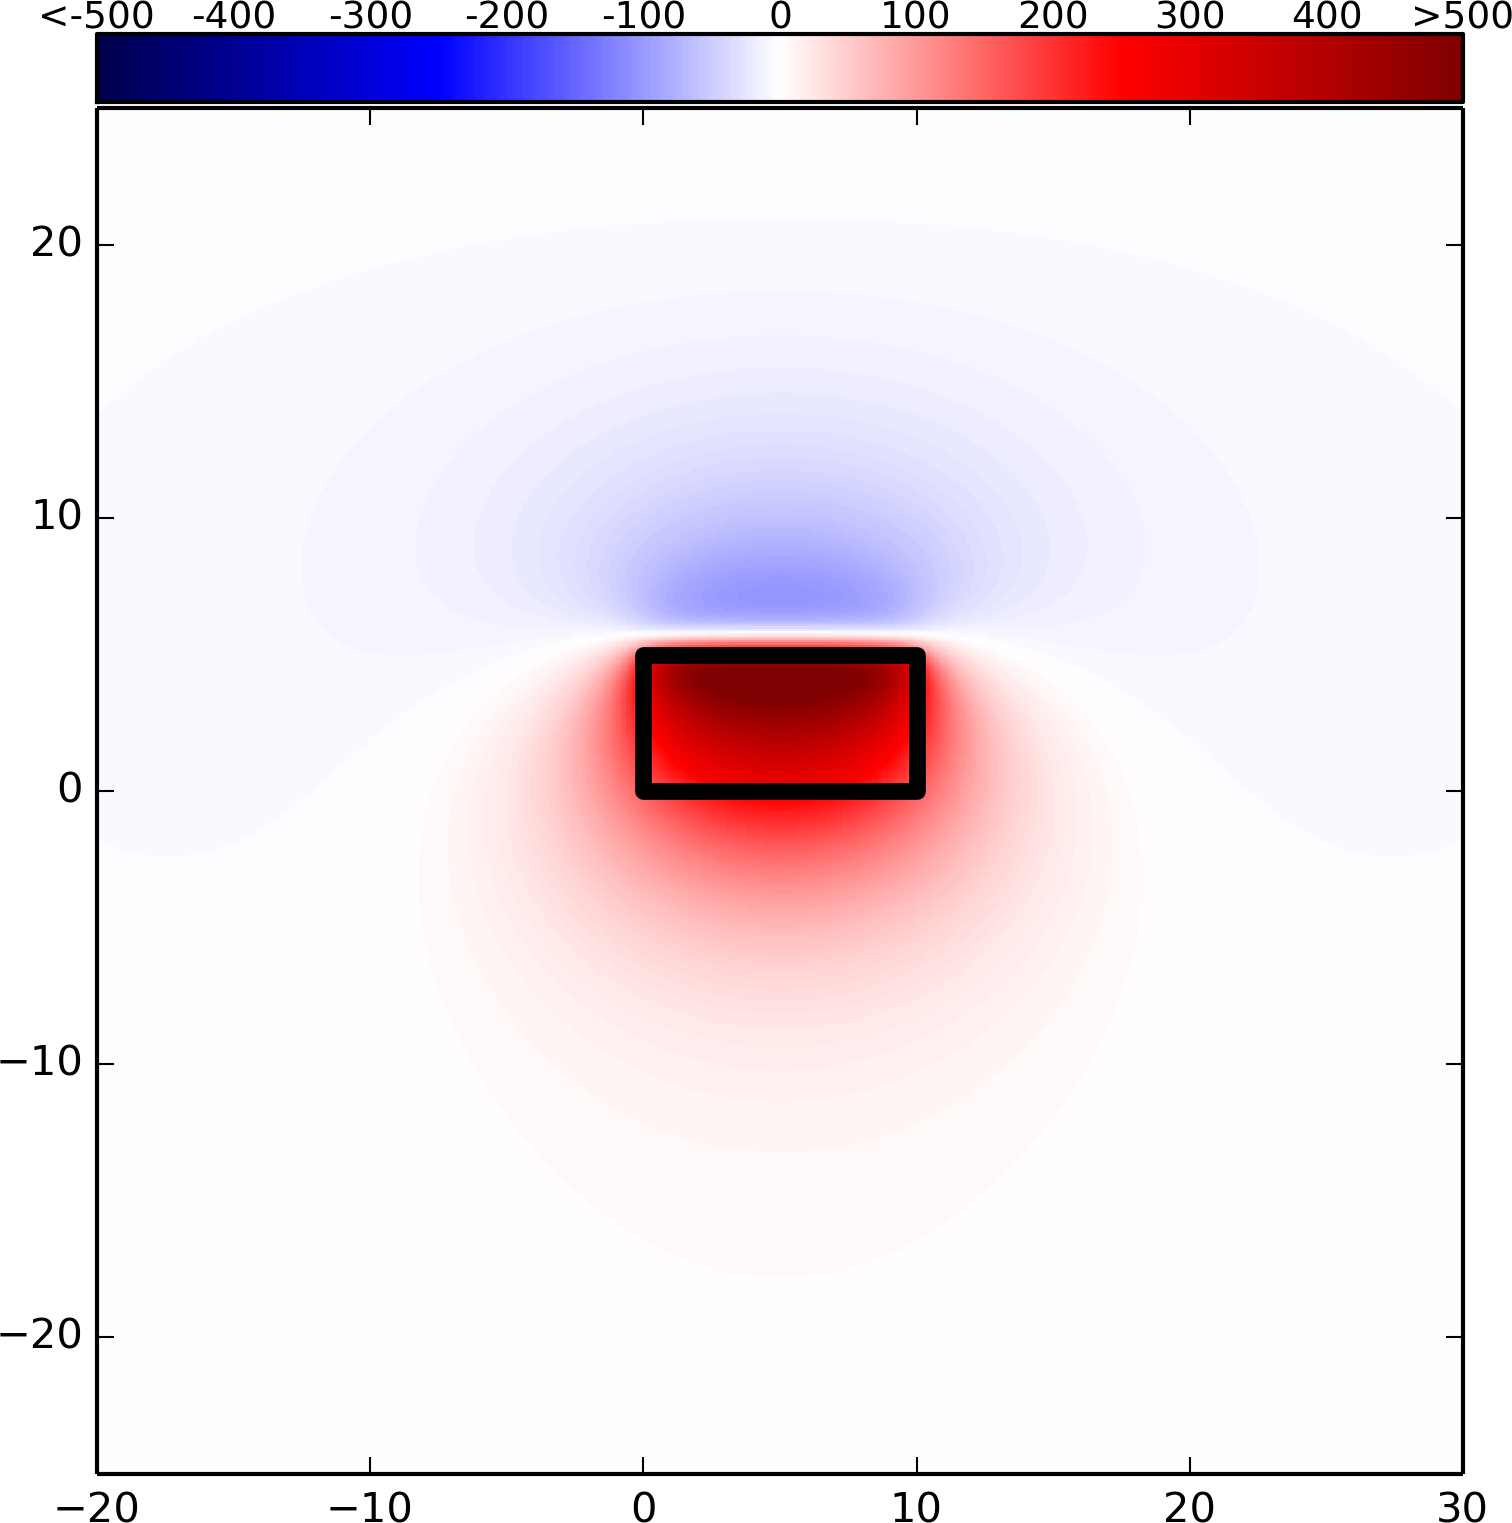
\includegraphics[width=1\textwidth]{graphics/dg_normal5_dip60_L10k_W10k_c10k_docs_trim}}
\par\end{center}%
\end{minipage}\hfill{}%
\begin{minipage}[t]{0.32\columnwidth}%
\begin{center}
\subfloat{\noindent \centering{}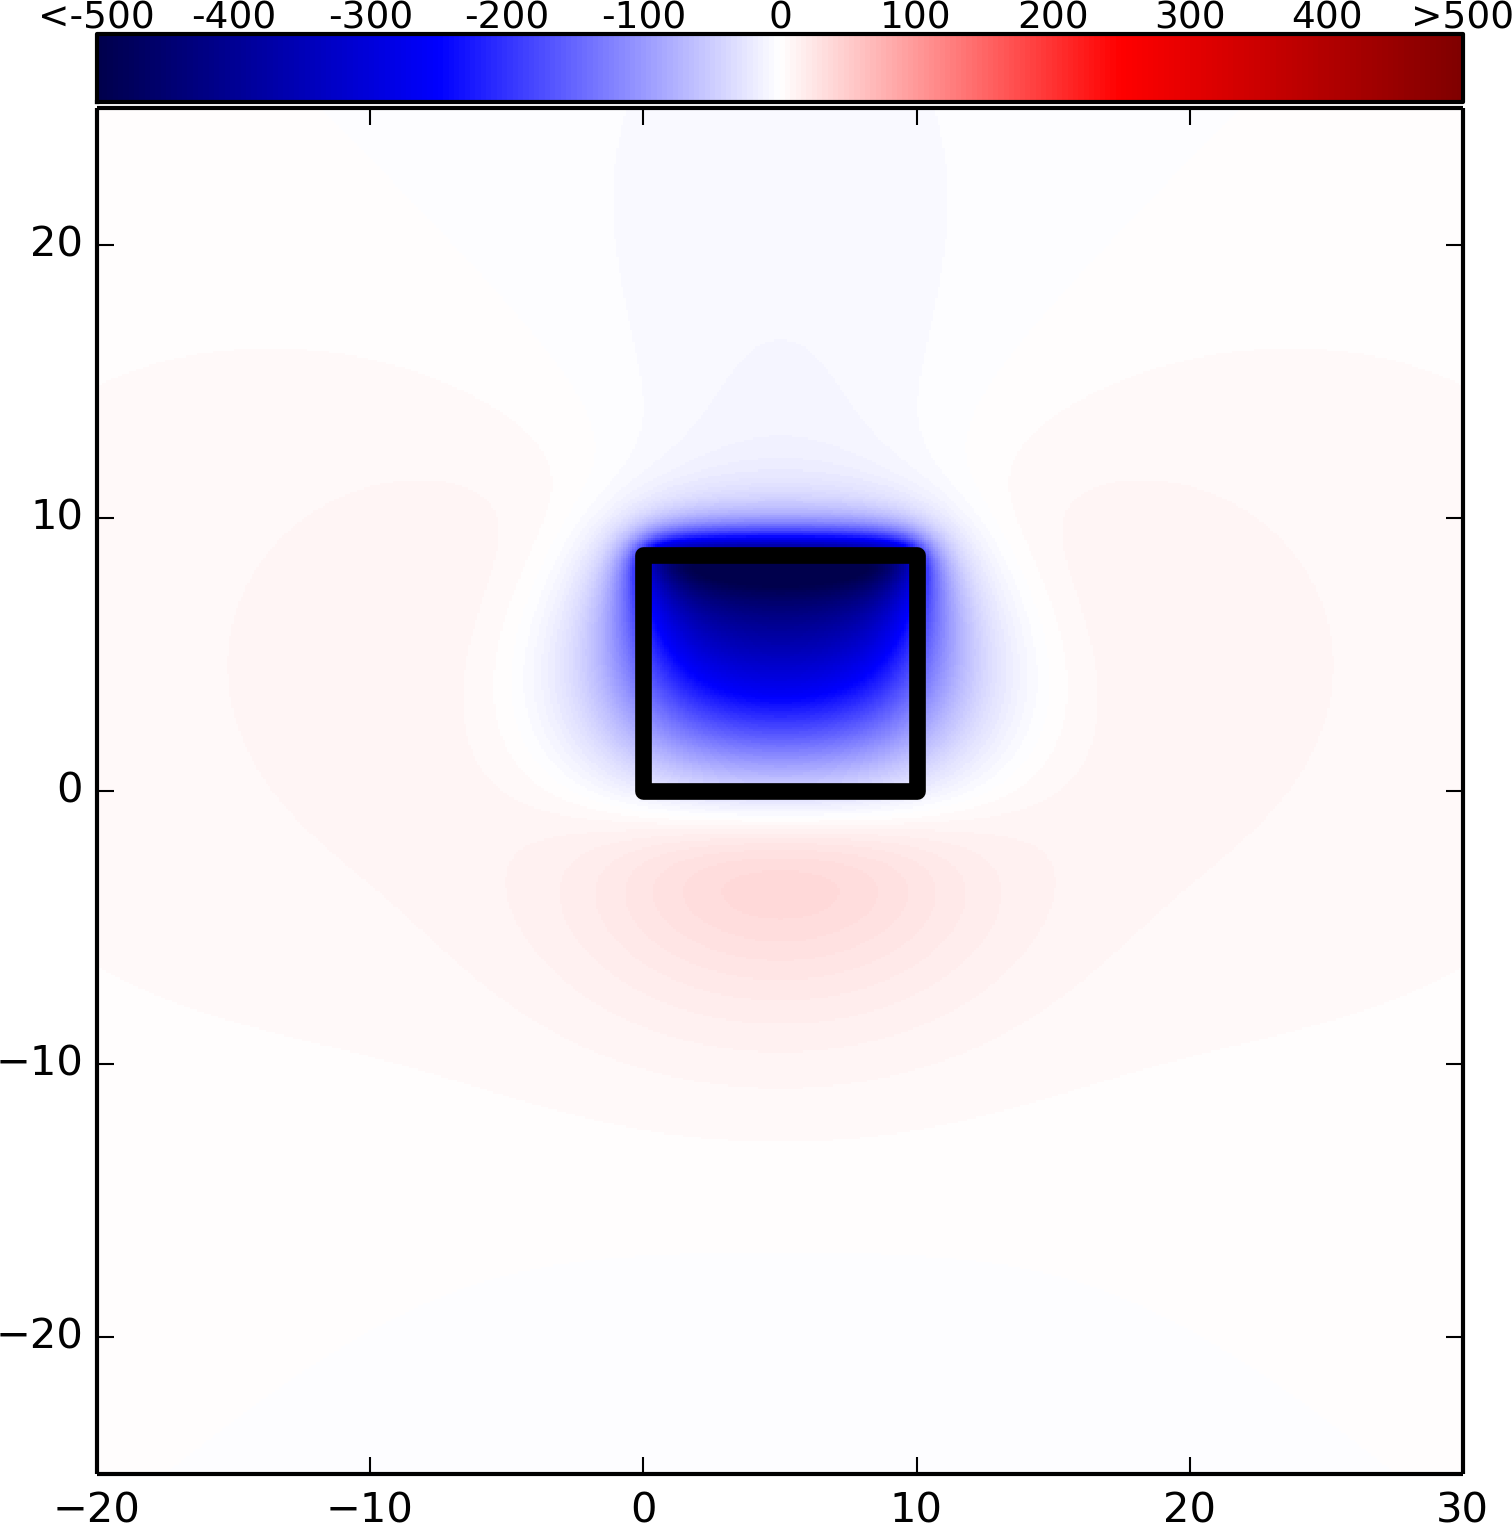
\includegraphics[width=1\textwidth]{graphics/dg_thrust5_dip30_L10k_W10k_c6k_docs_trim}}
\par\end{center}%
\end{minipage}

\caption{Gravitational anomalies for the fault elements in Figure \ref{fig:single_element_displacements},
colorbar units are $\mu gal$.\label{fig:single_element_gravity_changes}}
\end{figure}

\par\end{center}


\subsection{Topologically Realistic Examples}

The true power of QuakeLib lies in its ability to serve as the analytical
backbone for visualizing the results of Virtual Quake's simulated
seismic histories. The following example plots illustrate this point
by showing QuakeLib's tools applied over many fault elements involved
in a single simulated earthquake. The earthquakes visualized
below come from a simulation involving all major fault sections in
California, the UCERF2 model described in section \ref{sec:Fault_model}.


\subsubsection{Displacement Field}

Figure \ref{fig:Displacement_field} shows the vertical displacement field
on the surface as seen by an orbiting satellite for a very large (moment
magnitude 8.0) earthquake involving multiple sections of the San Andreas
Fault.

\begin{figure}
\centering{}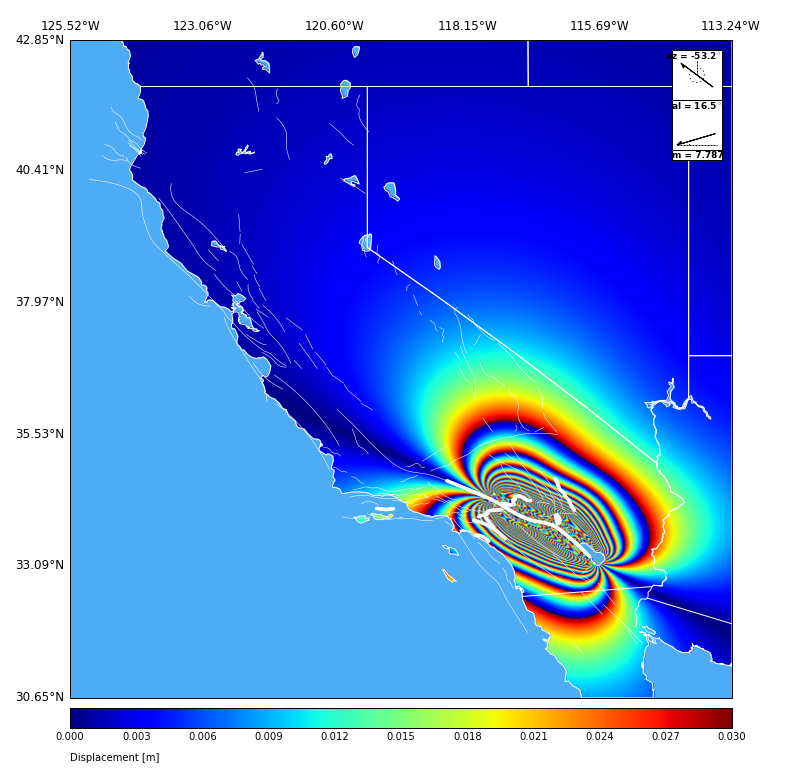
\includegraphics[width=1\textwidth]{graphics/dz_54358}\caption{\label{fig:Displacement_field}Simulated InSAR interferogram showing
vertical displacements for a large earthquake (moment magnitude 7.79)
involving multiple sections of the southern San Andreas Fault (thick
white lines), as seen by an orbiting satellite. }
\end{figure}



\subsubsection{Gravity Field Anomalies}

Figure \ref{fig:Gravity_field} shows co-seismic gravitational anomaly
field on the surface, as measured by an orbiting satellite
for the same simulated earthquake as Figure \ref{fig:Displacement_field}. 

\begin{figure}
\centering{}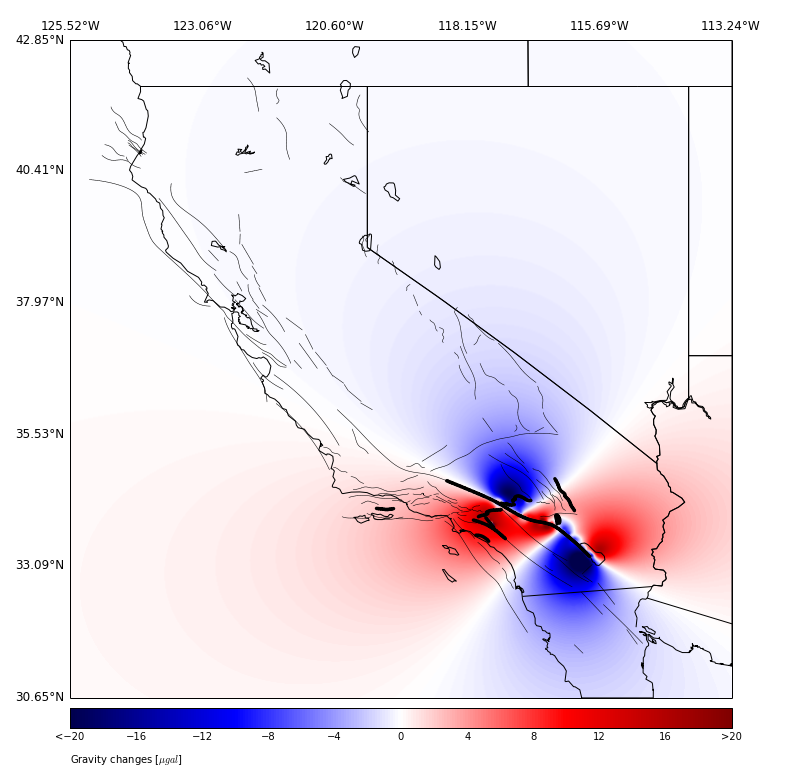
\includegraphics[width=1\textwidth]{graphics/dg_54358}\caption{\label{fig:Gravity_field}Simulated surface gravity anomalies for
the same simulated earthquake as in Figure \ref{fig:Displacement_field}. }
\end{figure}



\chapter{Getting Started and Installation\label{cha:Installation}}


\section{Introduction}

Virtual Quake and QuakeLib have been tested on Linux, Mac OS
X and several other UNIX based platforms. Virtual Quake has also
been successfully run in parallel on several XSEDE systems and commodity
cluster systems. You should have no problems compiling, installing,
and running Virtual Quake on most Unix-like systems. Virtual
Quake is currently only available as a source package that users
must compile on their own. The following sections will lead you through
the installation process.


\section{Getting Help}

For help, send e-mail to the Short Term Crustal Dynamics Mailing List \url{cig-short@geodynamics.org}.
You can subscribe to the Mailing List and view archived discussion
at the Geodynamics Mail Lists web page \url{http://geodynamics.org/cig/about/mailing-lists/}.
For bugs found in the manual or source code, or to make feature requests please use the Github issue tracker at \url{https://github.com/geodynamics/vq/issues}.


\section{System Requirements}

Installation of Virtual Quake requires a C++ compiler.  Optional requirements are the
headers and development libraries for
\begin{itemize}
\item MPI
\item OpenMP
\item HDF5
\item SWIG
\item CMake
\end{itemize}
You must also have Python 2.7 or greater installed.


\section{Obtaining Source}

To obtain the latest official release of Virtual Quake, go to the Geodynamics software package
web page \url{http://geodynamics.org/cig/software/vq}, download the source
archive and unpack it using the \texttt{tar} command:
\begin{verbatim}
$ tar xzf vq-1.1.0.tar.gz
\end{verbatim}

To get the latest development version of Virtual Quake, use git to make a copy of the repository:
\begin{verbatim}
$ git clone --recursive https://github.com/geodynamics/vq
\end{verbatim}

\section{\label{sec:Install}Installation Procedure}

After unpacking the source, use the following procedure to install
the Virtual Quake executable as well as the QuakeLib library
and the mesher program:
\begin{enumerate}
\item Navigate to the directory containing the Virtual
Quake source\texttt{.}~\\
\texttt{}~\\
\texttt{\$ cd vq}
\item Make the build directory and navigate to it.\\
\texttt{}~\\
\texttt{\$ mkdir build}~\\
\texttt{\$ cd build}
\item Use CMake to configure before compiling VQ.\texttt{}~\\
\texttt{}~\\
\texttt{\$ cmake ..}
\item Use make to build QuakeLib and the VQ binaries.\texttt{}~\\
\texttt{}~\\
\texttt{\$ make}
\item The final step is required only if the user intends to use the quakelib python module \texttt{}~\\
\texttt{\$ sudo make install}
\end{enumerate}
If you are content to run Virtual Quake from the build directory,
then you are done. Upon successful completion, the \texttt{make} command
creates two executables ``mesher'' and ``vq'' in the
\texttt{/build/src/} subdirectory. ``vq'' is the binary you will use to
run a Virtual Quake simulation, and the mesher program can create
fault models as described in Section \ref{sec:building_faults}.


\subsection{Mac OS X}

If you have a third party installation of python (e.g. from Homebrew
or MacPorts) Virtual Quake will build and install, but the Python
QuakeLib module may not work (failure will generally manifest itself as a segmentation fault). This is because CMake may build against
a different installation of Python than it runs Python scripts with. To fix this you can specify the Python installation to use when compiling QuakeLib with:
\begin{verbatim}
cmake -DPYTHON_EXECUTABLE=/.../python \
    -DPYTHON_LIBRARY=/.../libpython2.7.dylib \
    -DPYTHON_INCLUDE_DIR=/.../include/python2.7/ ..
\end{verbatim}

Be sure to change the paths to whatever is appropriate on your system.

\subsection{Install Locations}

QuakeLib libraries will be installed in standard library directories
based on your system configuration. CMake will generate a file named
\texttt{install\_manifest.txt} in the build directory detailing
the locations of installed files. The Virtual Quake binary is at
\texttt{build/src/vq}.


\subsection{Selecting a Compiler --- Multiprocessing\label{sec:Selecting-a-Compiler-Multiproc}}

Depending on the machine used to run VQ, you may need to change which
compiler CMake uses to compile VQ. For example, if the user wants
to compile VQ with gcc 3.3, execute cmake as shown below.
\begin{verbatim}
$ CC=gcc-3.3 CXX=g++-3.3 cmake ..
$ make
\end{verbatim}
To compile Virtual Quake and deploy it across multiple processors using MPI, execute cmake instead as:
\begin{verbatim}
$ CC=mpicc CXX=mpicxx cmake ..
$ make
\end{verbatim}

\subsection{Additional Tools}

While the following software is not necessary for the normal operation
of Virtual Quake, you may find it useful for accessing Virtual
Quake data in HDF5 files.

%
%\subsubsection{NumPy}
%
%NumPy is an extension to Python which adds support for multi-dimensional
%arrays for use in scientific computing. You may download NumPy from
%the NumPy home page \url{numpy.scipy.org}. To compile and install
%this extension, download it and issue the following commands after
%extracting it:
%\begin{verbatim}
%\$ cd~numpy-1.0
%\$~python~setup.py~install~-{}-prefix=\$HOME/cig
%\end{verbatim}
%Alternatively, under Debian Linux you can install the \texttt{python-numpy}
%package. On Gentoo Linux, NumPy is available in the \texttt{dev-python/numpy}
%build.
%

%\subsubsection{PyTables}
%
%PyTables is a package for managing hierarchical datasets and designed
%to efficiently and easily cope with extremely large amounts of data.
%PyTables is built on top of the HDF5 library, using the Python language
%and the NumPy package. After checking its dependencies, you may download
%PyTables from the PyTables home page \url{pytables.org}. To install,
%follow instructions on the installation page \url{http://pytables.github.io/usersguide/installation.html}. 


\subsubsection{HDFView}

HDFView is a visual tool written in Java for browsing and editing
HDF5 files. You may download it from the HDFView home page \url{hdf.ncsa.uiuc.edu/hdf-java-html/hdfview}.


\chapter{Running VQ\label{cha:Running_VQ}}


\section{Introduction}

Now that installation and testing is finished, we will get into the
specifics of building a fault model, compiling Virtual Quake,
and finally running a custom simulation. The following chapter serves
to illustrate the main features of a Virtual Quake simulation,
and will prepare the user for the examples in Chapter \ref{cha:Running_VQ}. 


\section{Basic Usage and Tests}

The main procedure for running a VQ simulation is to create
the fault model (see Sections
\ref{sec:Tutorial_single} and \ref{sec:Tutorial_multiple} for examples),
compile Virtual Quake following Section \ref{sec:Install} to
generate the executable, place the executable in the same folder as
the parameter files, and finally execute the program. 


\subsection{CMake Tests}

If you installed Virtual Quake according to Section \ref{sec:Install},
then you successfully compiled the QuakeLib library and the VQ and
mesher executables. CMake is used to configure the simulation program,
and also provides a test framework to ensure all parts of VQ are working as expected. To run the suite of tests use the following commands.
\begin{verbatim}
$ cd build/
$ make test
Running tests...
Test project /.../build
        Start   1: CondUnitTest
  1/230 Test   #1: CondUnitTest .............................   Passed    0.08 sec
        Start   2: FricUnitTest
  2/230 Test   #2: FricUnitTest .............................   Passed    0.09 sec
        Start   3: GreenUnitTest
  3/230 Test   #3: GreenUnitTest ............................   Passed    0.09 sec
        Start   4: OctreeTest
  4/230 Test   #4: OctreeTest ...............................   Passed    0.06 sec
        Start   5: UtilUnitTest
  5/230 Test   #5: UtilUnitTest .............................   Passed    0.15 sec
        Start   6: EventUnitTest
  6/230 Test   #6: EventUnitTest ............................   Passed    0.05 sec
        Start   7: GeomUnitTest
  7/230 Test   #7: GeomUnitTest .............................   Passed    0.05 sec
        Start   8: MetadataUnitTest
  8/230 Test   #8: MetadataUnitTest .........................   Passed    0.04 sec
        Start   9: RectBoundTest
  9/230 Test   #9: RectBoundTest ............................   Passed    0.04 sec
        Start  10: mesh_P1_none_12000
 10/230 Test  #10: mesh_P1_none_12000 .......................   Passed    0.01 sec
        Start  11: param_P1_none_12000
 11/230 Test  #11: param_P1_none_12000 ......................   Passed    0.01 sec
        Start  12: run_P1_none_12000
 12/230 Test  #12: run_P1_none_12000 ........................   Passed    0.05 sec
        Start  13: test_consistent_P1_none_12000
 13/230 Test  #13: test_consistent_P1_none_12000 ............   Passed    0.32 sec
        Start  14: test_slip_P1_none_12000
 14/230 Test  #14: test_slip_P1_none_12000 ..................   Passed    0.33 sec
        Start  15: test_interevent_P1_none_12000
 15/230 Test  #15: test_interevent_P1_none_12000 ............   Passed    0.31 sec
...
        Start 230: test_two_consistent_taper_renorm_3000
230/230 Test #230: test_two_consistent_taper_renorm_3000 ....   Passed    0.72 sec

100% tests passed, 0 tests failed out of 230

Total Test time (real) =  54.90 sec
\end{verbatim}
The final lines of the
output summarize the results from the unit tests and test simulations. 


\subsection{Explicit Test Simulation\label{sec:Single-Processor-Test}}

If you would rather explicitly follow the steps of building your own
fault model, generating the parameter files and running the simulation,
then you should consult the tutorial in Section \ref{sec:Tutorial_single}. 


\section{Advanced Usage}

Since the simulation physics and event model will work with any arbitrarily
complex fault model, advanced users can make Virtual Quake generate
simulated seismic histories for any fault system. The only requirement
for using VQ to simulate dynamics on an arbitrary fault network is
to prepare the input files. Chapter \ref{cha:Running_VQ} contains
examples that illustrate this procedure of defining fault geometry
and properties.


\subsection{Tuning Parameters\label{sec:tuning_parameters}}

Fault simulations must initially be tuned to correctly simulate actual
earthquakes. The primary tuning parameter in Virtual Quake is
the dynamic triggering factor $\eta$,
defined in Section \ref{sec:Event_Model}. The dynamic triggering
factor is used to encourage rupture propagation during a simulated
earthquake. This parameter acts to tune the rupture and
slipping properties of faults without requiring field measurements
of each fault's physical properties, a result of VQ's abstraction
and generality. Currently, this parameter is set globally for the
fault model.
%Figure \ref{fig:tuning_parameters} shows a comparison
%of simulation results for a range of these parameter values.
%
%\begin{center}
%\begin{figure}
%\begin{minipage}[t]{0.48\columnwidth}%
%\begin{center}
%\subfloat{\noindent \centering{}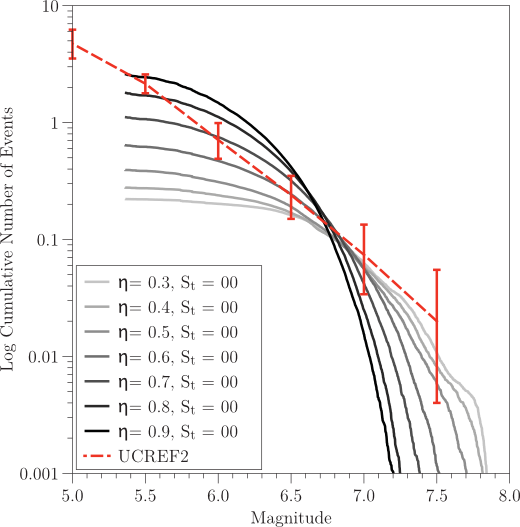
\includegraphics[width=1\textwidth]{graphics/tuning_parameters_1}}
%\par\end{center}
%
%\begin{center}
%\textbf{(a)}
%\par\end{center}%
%\end{minipage}\hfill{}%
%\begin{minipage}[t]{0.48\columnwidth}%
%\begin{center}
%\subfloat{\noindent \centering{}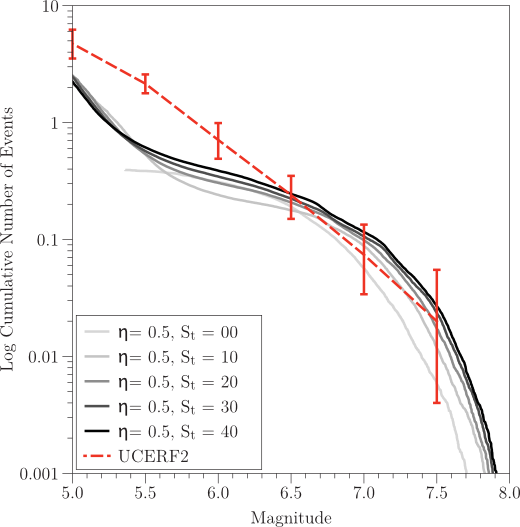
\includegraphics[width=1\textwidth]{graphics/tuning_parameters_2}}
%\par\end{center}
%
%\begin{center}
%\textbf{(b)}
%\par\end{center}%
%\end{minipage}\bigskip{}
%\begin{minipage}[t]{0.48\columnwidth}%
%\begin{center}
%\subfloat{\noindent \centering{}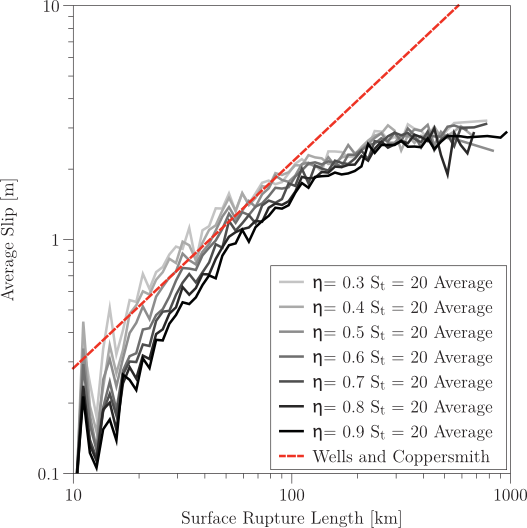
\includegraphics[width=1\textwidth]{graphics/tuning_parameters_3}}
%\par\end{center}
%
%\begin{center}
%\textbf{(c)}
%\par\end{center}%
%\end{minipage}\hfill{}%
%\begin{minipage}[t]{0.48\columnwidth}%
%\begin{center}
%\subfloat{\noindent \centering{}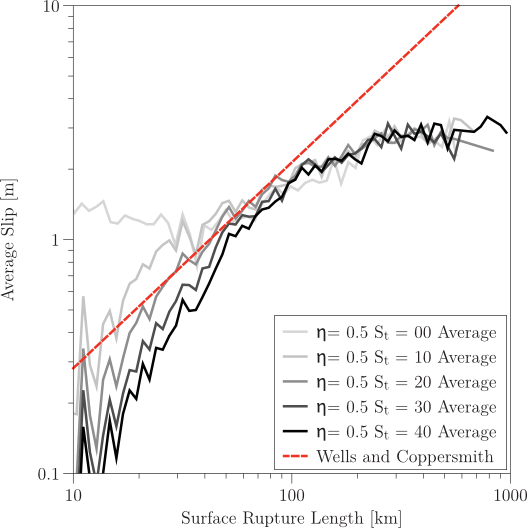
\includegraphics[width=1\textwidth]{graphics/tuning_parameters_4}}
%\par\end{center}
%
%\begin{center}
%\textbf{(d)}
%\par\end{center}%
%\end{minipage}
%
%\caption{The output from several VQ simulations over a range of dynamic triggering
%and slip-scaling threshold parameter values: (a) frequency-magnitude
%varying$\eta$; (b) frequency-magnitude varying $S_t$; (c) average
%slip-surface rupture length varying $\eta$; and (d) average slip-surface
%rupture length varying $S_t$. The dashed red line and error bars
%in (a) and (b) are the observed seismicity in California and 95\%
%confidence levels as reported by UCERF2 \cite{UCERF2}. The dashed
%red lines in (c) and (d) are observed relationships reported by Wells
%and Coppersmith \cite{Wells01081994}. \label{fig:tuning_parameters}}
%\end{figure}
%
%\par\end{center}


\subsection{Simulation Performance and Scaling\label{sec:element_size_discussion}}

Virtual Quake is designed to support parallel computing with OpenMP or MPI
and this section gives some quantitative results of deploying VQ in
multiprocessing environments. The key factors
determining the scope of the output and the simulation performance
are the number and size of the fault elements in the fault model.
The size of the meshed elements will affect both simulation accuracy
and computational resource requirements. The appropriate size of fault
elements for a given simulation depends on the desired minimum earthquake
magnitude and the available computational resources. 


\subsection{Element Size and Minimum Magnitude}

The relationship between element size and minimum magnitude is given
by:

\begin{equation}
M_{min}=\frac{2}{3}log_{10}(1e7\mu sL^{2})-10.7
\end{equation}


where $\mu$ is the Lam� parameter, s is the minimum slip distance,
and $L$ is the element size in meters. The minimum slip distance,
s, will depend on the orientation of the element, the total fault
size, and the interaction with other elements in the system, but will
generally range from approximately 0.1 to 1.0 meters. For example,
for the 12km x 12km fault described in Section \ref{sec:define_mesh_faults}
the minimum slip distance is 0.3 meters. Figure \ref{fig:min_magnitude_elem_size}
shows the relationship in VQ between element size and minimum earthquake
magnitude.

\begin{figure}
\subfloat[\label{fig:operations_per_element}Operations required to calculate
a single element-element stress interaction.]{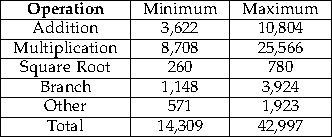
\includegraphics[width=0.48\textwidth]{graphics/Heien_Sachs_12_number_of_operations}

}\hfill{}\subfloat[\label{fig:min_magnitude_elem_size}Element size versus minimum event
magnitude.]{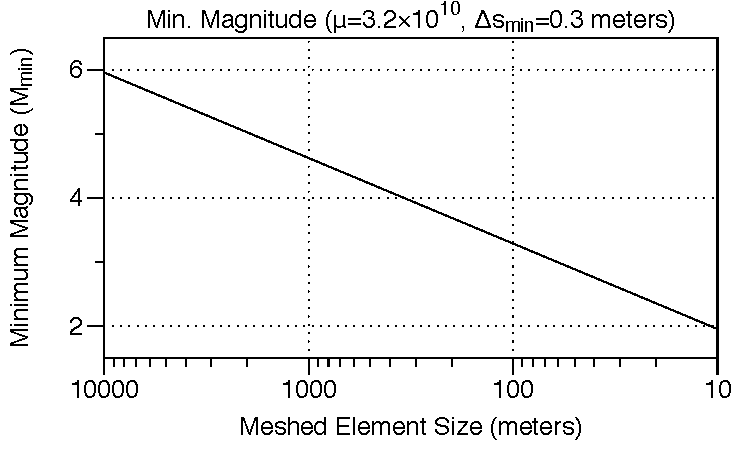
\includegraphics[width=0.48\textwidth]{graphics/min_magnitude}

}

\caption{Number of elements determines computational cost - this will vary depending on the relative rake and dip. Element size governs
simulated earthquake magnitude range.}
\end{figure}



%\subsection{Element Size and Required Memory}

The number of elements in a model will also affect the required memory.
%Since VQ uses a Barnes-Hut style approximation algorithm for fault
%interaction the actual memory required will depend on the accuracy
%of the approximation.
For non-approximated fault interaction in a
model with $N$ elements, the memory requirements are:

\begin{equation}
Memory=16N^{2}bytes
\end{equation}

%Because the degree of approximation possible with Barnes-Hut will vary depending on the system geometry it is not possible to give memory requirements. 

\begin{figure}
\subfloat[\label{fig:memory_vs_element_size_1}Element size determines computational
regime.]{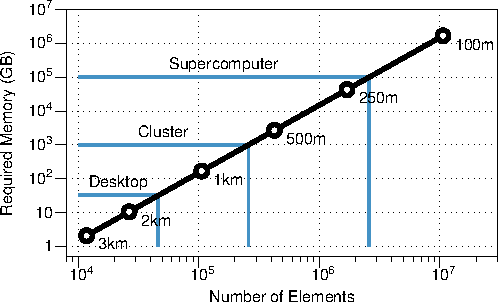
\includegraphics[width=0.48\textwidth]{graphics/Heien_Sachs_12_elements_vs_memory}

}\hfill{}\subfloat[\label{fig:memory_vs_element_size_2}Number of elements vs. memory
requirements with approximations.]{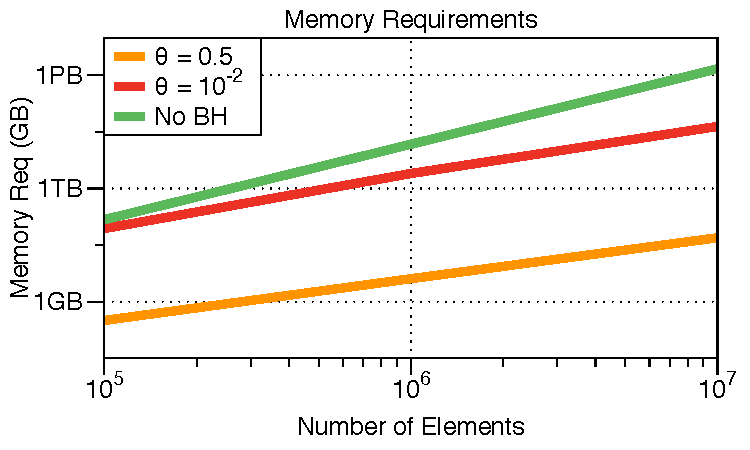
\includegraphics[width=0.48\textwidth]{graphics/memory_reqs}

}

\caption{Tradeoffs in element size and resource requirements.}
\end{figure}



%\subsection{Parallel Performance}
%
%The program flow in Figure \ref{fig:simulation_flow} shows three
%main communication points. The global nature of these communications
%is a bottleneck to simulation performance on a parallel system. 
%
%Figure \ref{fig:sim_breakdown} shows simulation run times for a 13,398
%element 100,000 year simulation on a simple cluster system using different
%numbers of processors. The cluster has 16 nodes, with two 2.4 GHz
%quad-core Xeon processors per node and a Gigabit ethernet network.
%For a single processor, most of the time is spent in the long term
%stress calculation and the initial Green's function
%calculations. As the number of processors increases these calculations
%scale well but the time spent in communication significantly rises.
%By 16 processors the majority of simulation time is spent communicating
%and there is very poor strong scalability.
%
%Figure \ref{fig:sim_comm_breakdown} shows the breakdown in time for
%different types of communication. For all numbers of processors, the
%majority of time is spent distributing stress values over the processors.
%This is required because the changes in stress during a rupture potentially
%lead to other elements rupturing. However, at a given rupture propagation
%step it is highly unlikely the rupture will spread a significant distance
%past where it already has traveled.
%
%\begin{figure}
%\subfloat[\label{fig:sim_breakdown}Parallel simulation time breakdown.]{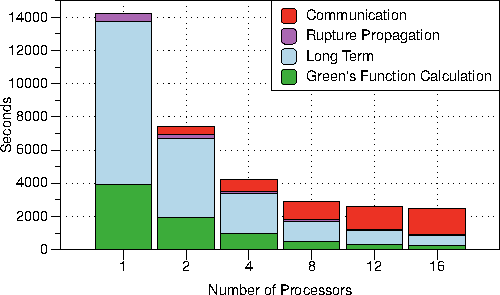
\includegraphics[width=0.48\textwidth]{graphics/Heien_Sachs_12_parallel_sim_time_breakdown}
%
%}\hfill{}\subfloat[\label{fig:sim_comm_breakdown}Parallel communication time breakdown.]{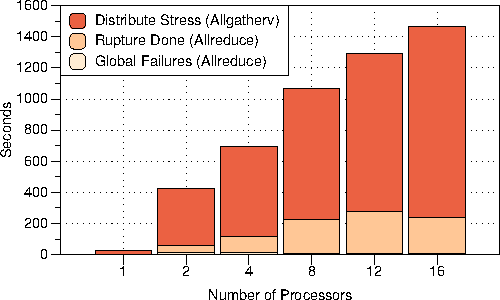
\includegraphics[width=0.48\textwidth]{graphics/Heien_Sachs_12_parallel_comm_time_breakdown}
%
%}
%
%\caption{Breakdown of total simulation time. }
%\end{figure}
%


\chapter{Tutorials \label{cha:Cookbooks}}


\section{Overview}

These tutorials are meant to serve as a guide to some of the types
of simulations VQ can perform. These cookbook examples are distributed
with the package under the \texttt{examples} directory. Each tutorial is a self-contained lesson in how to
use Virtual Quake. The tutorials increase in degree of complexity
from one to the next. In the last section, we demonstrate how to construct
the entire California fault system for large scale simulations.


\subsection{Prerequisites}

Before you begin any of the tutorials, you will need to install Virtual
Quake following the instructions in Chapter \vref{cha:Installation}.
If you do not wish to create your own mesh, the meshes
are also provided as part of the tutorial. 


\section{Building a Fault Model\label{sec:building_faults}}

VQ uses a mesher program for fault model file manipulation.
The mesher imports one or more trace files, manipulates
them based on user arguments and exports one or more files to be used
as input files for a VQ simulation. After following install
instructions in Section \ref{sec:Install}, the mesher program is
compiled to an executable located at \texttt{build/src/mesher}.
This program is called by the shell scripts in the examples below
to generate a fault model for VQ. See Section \vref{cha:Appendix-C:Mesher_Parameters}
for more information on the options for the mesher program.

The next sections give examples
and describe the model files that the mesher creates. For both files,
each commented line describes the parameter in the corresponding column
of the uncommented line immediately following the comments. See Section
\vref{cha:Appendix-A:-Input} and Section \vref{sec:Trace-File-Format}
for more information on the input fault model files and parameters.


\subsection{Trace File}

The basic outline for a fault trace file is given in Section
\vref{sec:Fault_model}. The trace file specifies the fault geometry
and physical parameters. An example is printed below.
\begin{verbatim}
 # fault_id: ID number of the parent fault of this section
 # num_points: Number of trace points comprising this section
 # section_name: Name of the section
 0 2 One_Fault_Example
 # latitude: Latitude of trace point
 # longitude: Longitude of trace point
 # altitude: Altitude of trace point (meters)
 # depth_along_dip: Depth along dip (meters)
 # slip_rate: Slip rate at trace point (centimeters/year)
 # aseismic: Fraction of slip that is aseismic at point
 # rake: Fault rake at trace point (degrees)
 # dip: Fault dip at trace point (degrees)
 # lame_mu: Lame's mu parameter at trace point (Pascals)
 # lame_lambda: Lame's lambda parameter at trace point (Pascals)
 0 0 0 12000 1 0 180 90 3e+10 3.2e+10
 0 0.1078 0 12000 1 0 180 90 3e+10 3.2e+10
\end{verbatim}

\subsection{Example Traces}

The \texttt{examples/fault\_traces/} folder contains the 
fault traces used in the examples below. In addition, we provide
trace files for all of California's major fault sections in the subfolder
\texttt{fault\_traces/ca\_traces/}.


\subsection{Friction Parameters}

Virtual Quake uses established scaling laws to determine certain
model parameters and initial conditions. Past simulations required
that the user specify the stress parameters on each element then run
the simulation based on this. However, the parameters that produce
realistic results depend strongly on the model fault geometry, size
of fault elements and friction properties. Furthermore these parameters
can be easily modified to produce arbitrary fault behavior. Rather
than require the user to specify these parameters, they are internally
calculated by VQ to match established physical laws and empirical
observations.

\subsection{Simulation Parameter File}

The main simulation input file is the parameter file. This file tells
the simulator where the fault model files are located, sets various
simulation variables, and specifies the output of the simulation.
An example parameter file template is located in \texttt{examples/}.


\subsection{Producing a Fault Model\label{sec:Using-Mesher}}

The first step is to use \texttt{setup\_mesh.sh} to generate the fault
trace file, and the second step is to edit the simulation parameter
file ``params.d''. This method is illustrated in the tutorials in
the following sections.


\subsection{Using the Mesher}

The mesher is called on the command line.  The following runtime options are supported:

\begin{verbatim}
./mesher [options]
-s FILE, --print_statistics=FILE
	Print statistics regarding final model to the specified file.
-m, --merge_duplicate_verts
	Merge duplicate vertices after importing files.
-d, --delete_unused
	Delete unused vertices after importing files.

FILE IMPORT
-i FILE, --import_file=FILE
	Specify a model file to import and merge. Must have a paired import_file_type.
-j TYPE, --import_file_type=TYPE
	Specify a model file type for importing. Must have a paired import_file.
-l SIZE, --import_trace_element_size=SIZE
	Specify the element size (in meters) to use for trace file meshing. Must have a paired trace type file import.
-t METHOD, --taper_trace_method=METHOD
	Specify the how to taper the imported trace when meshing. Must have a paired trace type file import.
-C FILE, --import_eqsim_condition=FILE
	Specify an EQSim condition file to import for the model.
-F FILE, --import_eqsim_friction=FILE
	Specify an EQSim friction file to import for the model.
-G FILE, --import_eqsim_geometry=FILE
	Specify an EQSim geometry file to import for the model.

FILE EXPORT
-e FILE, --export_file=FILE
	Specify a file to export the completed model to. Must have a paired export_file_type.
-f TYPE, --export_file_type=TYPE
	Specify a file type to export the completed model. Must have a paired export_file.
-D FILE, --export_eqsim_condition=FILE
	Specify an EQSim condition file to export for the model.
-R FILE, --export_eqsim_friction=FILE
	Specify an EQSim friction file to export for the model.
-M FILE, --export_eqsim_geometry=FILE
	Specify an EQSim geometry file to export for the model.
\end{verbatim}

\subsubsection{Parameter File}

Copy the \texttt{example\_params.d} file into the same folder as the mesher generated model.
Edit the parameter file so the simulation parameters are set correctly for the current run. 


\section{Single Element Tutorial\label{sec:Tutorial_single}}


\subsection{Overview}

This tutorial is the simplest possible implementation of Virtual Quake.
In this tutorial we will build the trace file for a single vertical
strike-slip fault element, then use this to build a fault model with
the mesher program and run this simulation for 10,000 years. 


\subsection{Creating Input Files}

We are going to create a new fault trace file for this single element.
The only data we need for this are the latitude and longitude of the
endpoints of our element. For this example we will use the following
coordinates (37.83,-122.4797) and (37.803,-122.4765). These endpoints
give a 3km fault element that runs parallel to and directly under the
Golden Gate Bridge in San Francisco. The trace file is printed below
and the fault element is shown above ground in Figure \ref{fig:Golden_Gate_single}.
\begin{verbatim}
 # fault_id: ID number of the parent fault of this section
 # num_points: Number of trace points comprising this section
 # section_name: Name of the section
 0 2 One_Fault_GG_Example
 # latitude: Latitude of trace point
 # longitude: Longitude of trace point
 # altitude: Altitude of trace point (meters)
 # depth_along_dip: Depth along dip (meters)
 # slip_rate: Slip rate at trace point (centimeters/year)
 # aseismic: Fraction of slip that is aseismic at point
 # rake: Fault rake at trace point (degrees)
 # dip: Fault dip at trace point (degrees)
 # lame_mu: Lame's mu parameter at trace point (Pascals)
 # lame_lambda: Lame's lambda parameter at trace point (Pascals)
 37.83 -122.4797 0 3000 1 0 180 90 3e+10 3.2e+10
 37.803 -122.4765 0 3000 1 0 180 90 3e+10 3.2e+10
\end{verbatim}
To create the input files, we use the mesher program as follows (arguments
explained in Section \ref{sec:building_faults}).
\begin{verbatim}
$ cd examples
$ mkdir golden_gate
$ cd golden_gate
$ ../../build/src/mesher \
--import_file=../fault_traces/golden_gate.txt \
--import_file_type=trace \
--import_trace_element_size=3000 \
--taper_fault_method=none \
--export_file=golden_gate_3000.txt \
--export_file_type=text \
--export_file=golden_gate_3000.kml \
--export_file_type=kml \
--print_statistics=statistics_3000.txt
\end{verbatim}

This generates several output files as listed by the command line
output shown below.

\begin{verbatim}
*** Summary of edits ***
File import ../fault_traces/golden_gate.txt with type trace... done.
File export golden_gate_3000.txt with type text... done.
File export golden_gate_3000.kml with type kml... done.
Print statistics to statistics_3000.txt
\end{verbatim}

\begin{figure}
\centering{}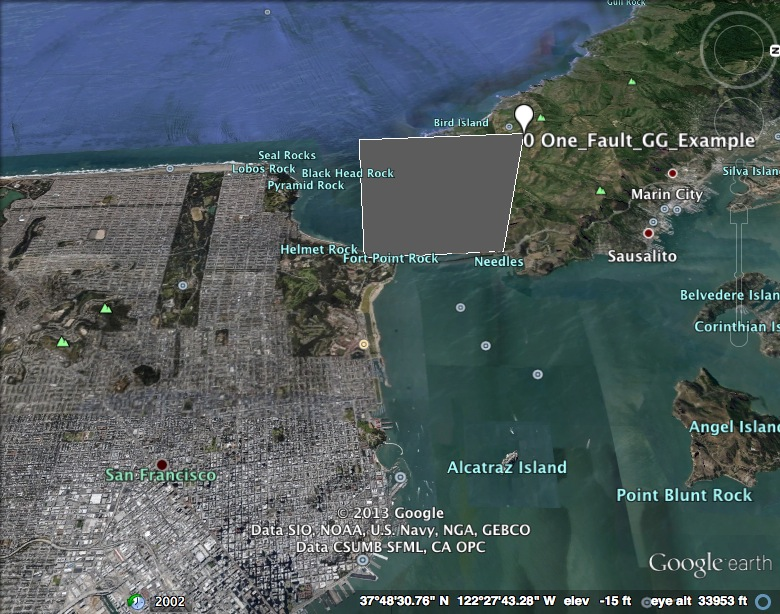
\includegraphics[width=0.72\textwidth]{graphics/One_Fault_Golden_Gate}\caption{\label{fig:Golden_Gate_single}Single 3km x 3km fault element running
under the Golden Gate Bridge in San Francisco, shown above ground.
This plot was generated by Google Earth from the mesher generated KML file.}
\end{figure}


Trace values for the faults in California are taken from Ward's ALLCAL2 model \cite{Ward01112012}, more information is available at \href{http://scec.usc.edu/research/eqsims/documentation.html}{http://scec.usc.edu/research/eqsims/documentation.html}. 


\subsection{Edit Parameter File}

The parameter file must be in the same directory (\texttt{examples/golden\_gate/}). Make sure the parameter file \texttt{params.d} is as shown below:
\begin{verbatim}
sim.version                       = 2.0 
sim.time.end_year                 = 10000 
sim.greens.method                 = standard 
sim.greens.use_normal             = false 
sim.friction.dynamic              = 0.5 
sim.file.input                    = golden_gate_3000.txt 
sim.file.input_type               = text 
sim.file.output_event             = events_3000.txt 
sim.file.output_sweep             = sweeps_3000.txt 
sim.file.output_event_type        = text
\end{verbatim}

\subsection{Running VQ}

With the generated fault mesh and and parameter file we can run the simulation.
To do so, call the vq executable (single processor) and pass the parameter file as a command line argument:
\begin{verbatim}
$ ../../build/src/vq ./params.d
\end{verbatim}

You should see output similar to:

\begin{verbatim}
# *** MPI CPU count           : 1
# Initializing blocks.
# To gracefully quit, create the file quit_vq in the run directory.
# Calculating Greens function with the standard Okada class.
# Greens function took 0.00187707 seconds.
# Greens shear matrix takes 128 bytes.
# Greens normal matrix takes 128 bytes.
# To access the event output file during the simulation, pause 
# by creating the file pause_vq.  Delete the file to resume.
# Writing events in format text to file events_3000.txt
# Plugin requested simulation end: Block stress calculation
 #                   Timer Name  AvgCounts        Min        Max       Mean     StdDev 
 0                   Total Time          1      0.053      0.053      0.053      0.000
 1             Init and Cleanup          2      0.010      0.010      0.010      0.000
 2                 Comm Barrier          2      0.000      0.000      0.000      0.000
 3     Block stress calculation        748      0.003      0.003      0.003      0.000
 4     Propagate event ruptures        748      0.019      0.019      0.019      0.000
 5                  Data Writer        748      0.018      0.018      0.018      0.000
\end{verbatim}

\subsection{Results}

The output data will be in \texttt{events\_3000.txt} and \texttt{sweeps\_3000.txt}.
For more details about the file contents, see Appendix
\ref{chap:Virtual-Quake-Output}. The results are not very exciting,
there is one earthquake that occurs regularly due to constant backslip.
But this illustrates setting up a Virtual Quake simulation start
to finish.


\section{Tutorial Using Multiple Elements\label{sec:Tutorial_multiple}}


\subsection{Overview }

Now we will repeat the single vertical strike-slip fault tutorial
from the previous section, but we will break up the fault into multiple
elements. 


\subsection{Creating Input Files}

For this tutorial, changing the element size to 1000 meters instead of 3000 meters will divide the fault into a 3 by 3 set of elements.  The command to do so is shown below:

\begin{verbatim}
$ cd examples/golden_gate
$ ../../build/src/mesher \
--import_file=../fault_traces/golden_gate.txt \
--import_file_type=trace \
--import_trace_element_size=1000 \
--taper_fault_method=none \
--export_file=golden_gate_1000.txt \
--export_file_type=text \
--export_file=golden_gate_1000.kml \
--export_file_type=kml \
--print_statistics=statistics_1000.txt
\end{verbatim}

Which should result in the following output:

\begin{verbatim}
*** Summary of edits ***
File import ../fault_traces/golden_gate.txt with type trace... done.
File export golden_gate_1000.txt with type text... done.
File export golden_gate_1000.kml with type kml... done.
Print statistics to statistics_1000.txt
\end{verbatim}

We will copy the previous \texttt{params.d} file to \texttt{params\_multiple.d} and edit it to match the new file names, as shown below:
\begin{verbatim}
sim.version                       = 2.0 
sim.time.end_year                 = 10000 
sim.greens.method                 = standard 
sim.greens.use_normal             = false 
sim.friction.dynamic              = 0.5 
sim.file.input                    = golden_gate_3000.txt 
sim.file.input_type               = text 
sim.file.output_event             = events_3000.txt 
sim.file.output_sweep             = sweeps_3000.txt 
sim.file.output_event_type        = text
\end{verbatim}

\begin{figure}
\centering
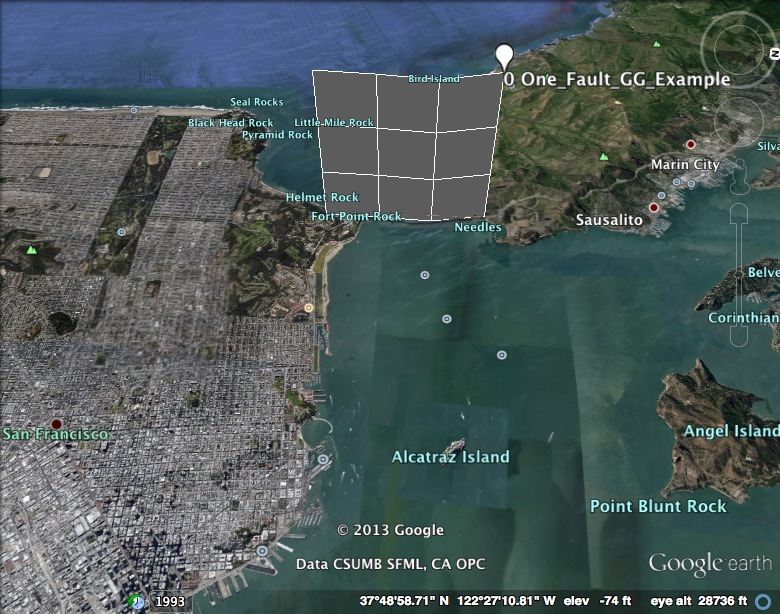
\includegraphics[width=0.72\textwidth]{graphics/Golden_Gate_Multi_Element.jpg}\caption{\label{fig:Golden_Gate_multiple}The same 3km x 3km fault section
from figure \ref{fig:Golden_Gate_single} but meshed into 1km x 1km
elements. This plot was generated by Google Earth from the mesher output KML file.}
\end{figure}


\subsection{Running VQ}

Again we run the simulation by calling the vq executable:
\begin{verbatim}
$ ../../build/src/vq ./params_multiple.d
\end{verbatim}

Output should be similar to the previous simulation:
\begin{verbatim}
# *** MPI CPU count           : 1
# Initializing blocks.
# To gracefully quit, create the file quit_vq in the run directory.
# Calculating Greens function with the standard Okada class.
# Greens function took 0.00388789 seconds.
# Greens shear matrix takes 1.125 kilobytes.
# Greens normal matrix takes 1.125 kilobytes.
# To access the event output file during the simulation, pause 
# by creating the file pause_vq.  Delete the file to resume.
# Writing events in format text to file events_1000.txt
# Plugin requested simulation end: Block stress calculation
 #                   Timer Name  AvgCounts        Min        Max       Mean     StdDev 
 0                   Total Time          1      0.228      0.228      0.228      0.000
 1             Init and Cleanup          2      0.005      0.005      0.005      0.000
 2                 Comm Barrier          2      0.000      0.000      0.000      0.000
 3     Block stress calculation        748      0.009      0.009      0.009      0.000
 4     Propagate event ruptures        748      0.124      0.124      0.124      0.000
 5                  Data Writer        748      0.089      0.089      0.089      0.000
\end{verbatim}

Note the Greens shear and normal matrices now require 1.125 KB of memory instead of 128 bytes of memory as in the previous simulation.  This is because the simulation now has 9 elements and a correspondingly larger Green's matrix.

\subsection{Results}

The output data is stored in \texttt{events\_1000.txt} and \texttt{sweeps\_1000.txt}. For more details about the file contents, see Appendix
\ref{chap:Virtual-Quake-Output}.

\section{Multiple Fault Sections}


\subsection{Overview}

This tutorial explores a VQ simulation involving
two neighboring fault sections --- each 15km long and 12km deep meshed
into 3km by 3km elements. We will also use larger fault elements than
the previous example, which raises the lower bound for magnitudes
in the output data set. Furthermore, we now will be simulating the
interaction between 40 elements so the computational resource requirements
grow as well (see Section \ref{sec:element_size_discussion} for a
detailed discussion).

\subsection{Input Files}

We will use another trace file that is provided with the VQ package.
This trace file specifies two neighboring vertical strike slip faults 
that intersect at the Earth and Physical Sciences building
on campus at the University of California, Davis, shown in Figure
\ref{fig:Davis_2_fault}. We generate the mesh with the following
commands.
\begin{verbatim}
$ cd examples
$ mkdir two_fault
$ cd two_fault
$ ../../build/src/mesher \
--import_file=../fault_traces/multiple_fault_trace.txt \
--import_file_type=trace \
--import_trace_element_size=3000 \
--taper_fault_method=none \
--export_file=two_fault_3000.txt \
--export_file_type=text \
--export_file=two_fault_3000.kml \
--export_file_type=kml \
--print_statistics=statistics_3000.txt
\end{verbatim}
Which should output the following.
\begin{verbatim}
*** Summary of edits ***
File import ../fault_traces/two_fault_1.txt with type trace... done.
File import ../fault_traces/two_fault_2.txt with type trace... done.
File export two_fault_3000.txt with type text... done.
File export two_fault_3000.kml with type kml... done.
Print statistics to statistics_3000.txt
\end{verbatim}

Next, create the \texttt{params.d} file as below:
\begin{verbatim}
 sim.version                       = 2.0
 sim.time.end_year                 = 10000
 sim.greens.method                 = standard
 sim.greens.use_normal             = false
 sim.friction.dynamic              = 0.5
 sim.file.input                    = two_fault_3000.txt
 sim.file.input_type               = text
 sim.file.output_event             = events_3000.txt
 sim.file.output_sweep             = sweeps_3000.txt
 sim.file.output_event_type        = text
\end{verbatim}
\begin{figure}
\centering{}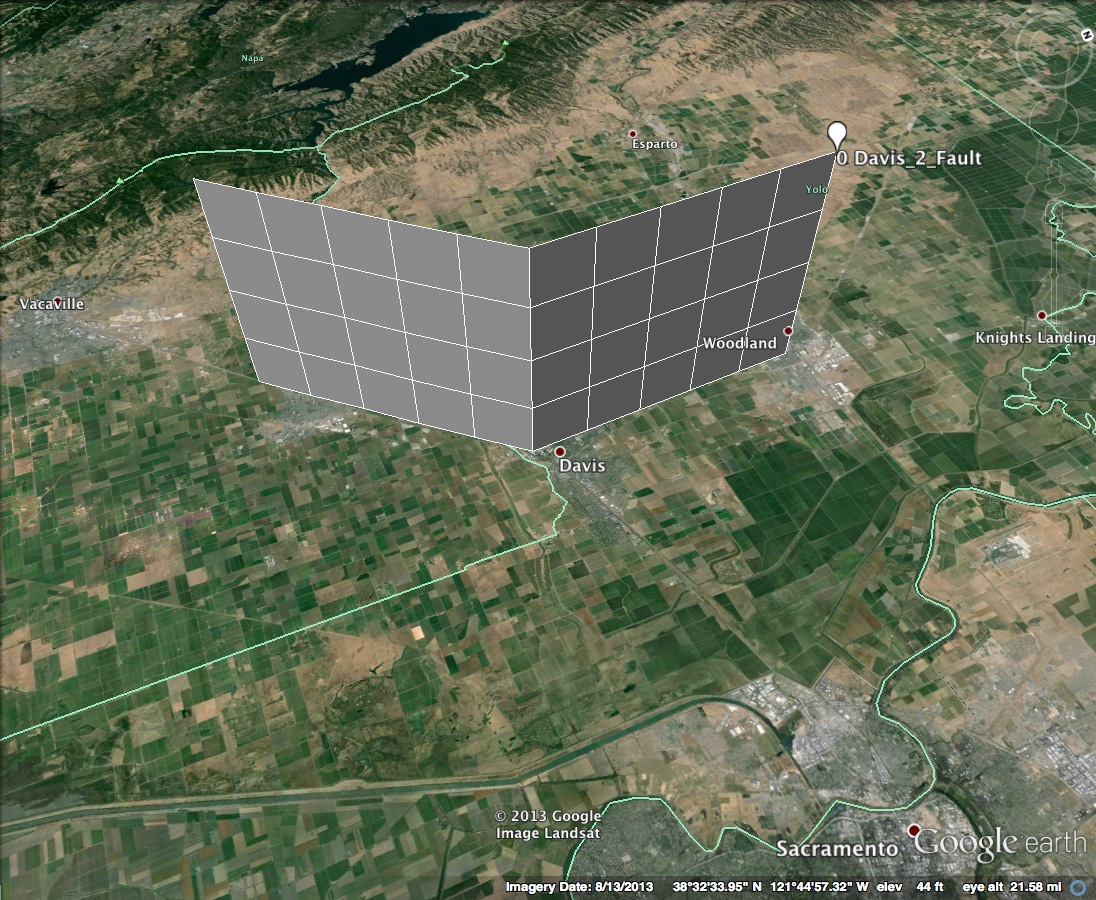
\includegraphics[width=0.72\textwidth]{graphics/Davis_2_Fault}\caption{\label{fig:Davis_2_fault}Two fault sections that meet at the UC Davis
campus. The fault sections are 15km x 12km and meshed into 3km x 3km
elements. This plot was generated by Google Earth from the mesher output KML file.}
\end{figure}

\subsection{Running VQ}

Again we run the simulation on a single processor by simply executing
the vq executable:
\begin{verbatim}
$ ../../build/src/vq ./params.d
\end{verbatim}
To instead run VQ in parallel on 2 or more processors/cores with MPI, use:
\begin{verbatim}
$ mpirun -np 2 ../../build/src/vq ./params.d
\end{verbatim}
The output from an MPI simulation should be identical that from a single processor simulation.

\subsection{Results}

The output data is stored in \texttt{events\_3000.txt} and \texttt{sweeps\_3000.txt}. For more details about the file contents, see Appendix
\ref{chap:Virtual-Quake-Output}.


\section{Building the full California Fault Model}
\subsection{Overview}

In the examples folder we also provide all the major fault traces in California and an executable script that can use them to build a full fault model. To build the full California fault model, execute the following commands to mesh the model into 3km elements:

\begin{verbatim}
$ cd examples/ca_model/
$ ./gen_ca_model.sh 3000
\end{verbatim}

Next, create an appropriate parameter file and run VQ as shown in the previous sections.  Note that the full CA simulation requires a fair amount of memory and may take several hours to finish.  Progress will be reported during the simulation if the \texttt{sim.system.progress\_period} parameter is set to a nonzero value (unit is seconds).



\section{Virtual Quake Data Analysis Tutorial (PyVQ) \label{sec:pyvq}}
\subsection{Overview}

Section \ref{sec:quakelib_tour} showed plots of gravity changes and an InSAR interferogram for a selected simulated earthquake. These plots that analyze simulation data utilize the python interface to the QuakeLib library, specifically a python module named quakelib that is generated during the final step of compiling Virtual Quake (when using the command ``sudo make install'', see section \ref{sec:Install}). In the following sections we describe how to make plots with Virtual Quake data using the pyvq script in the pyvq directory.

The set of simulation data analysis plotting scripts are located in the pyvq folder, and accessing by calling the python script pyvq.py with various command line arguments. The functionality is briefly explained in the README\_PYVQ file and discussed in further detail here. The full list of possible pyvq parameters is given in section \ref{sec:pyvq_params}.

\subsection{Simulation Statistics Plots}

To generate a frequency magnitude plot from your simulation file (hdf5), located at ``path/to/sim\_file.h5'', simply execute the shell command (in one line):

\begin{verbatim}
$ python path/to/vq/pyvq/pyvq.py --event_file path/to/sim_file.h5 --event_file_type 
     'hdf5' --plot_freq_mag 1
\end{verbatim}

If you generated a text file from your simulation, simply use instead: 

\begin{verbatim}
$ python path/to/vq/pyvq/pyvq.py --event_file path/to/sim_file.txt --event_file_type 
     'text' --plot_freq_mag 1
\end{verbatim}

This saves the plot to a file with the filename chosen from the name of the simulation file and the type of plot being drawn, Figure \ref{fig:freq_mag}.

\begin{figure}
\centering{}
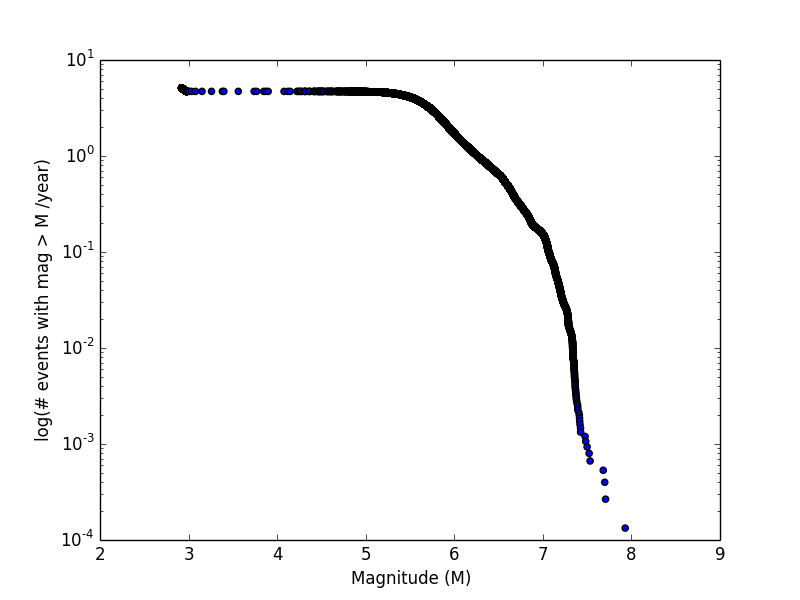
\includegraphics[width=0.7\textwidth]{graphics/freq_mag_example.png}
\caption{\label{fig:freq_mag} Example frequency-magnitude distribution.}
\end{figure}

To plot both the magnitude-rupture area and magnitude-mean slip distributions (Figure \ref{fig:mag_area_slip}) simply execute:

\begin{verbatim}
$ python path/to/vq/pyvq/pyvq.py --event_file path/to/sim_file.h5 --event_file_type 
     'hdf5' --plot_mag_rupt_area --plot_mag_mean_slip
\end{verbatim}

\begin{figure}
\centering{}
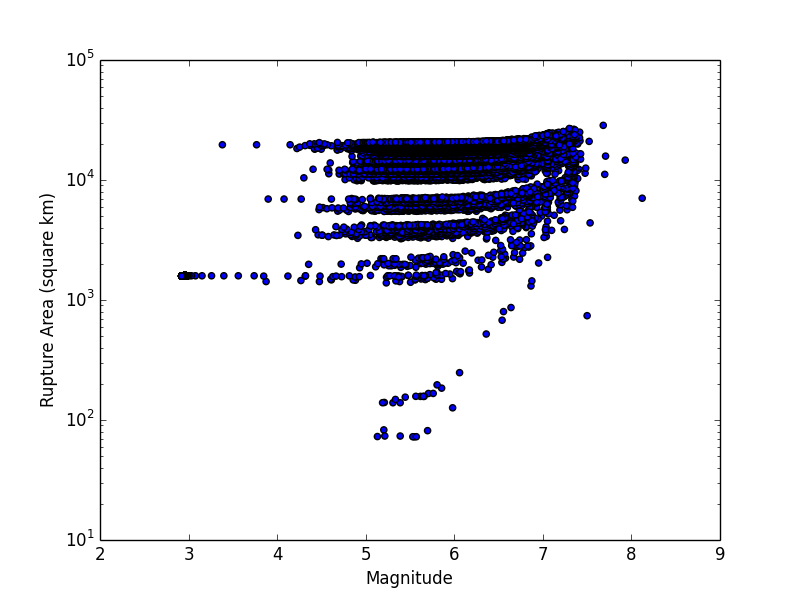
\includegraphics[width=0.49\textwidth]{graphics/mag_rupt_area_example.png}
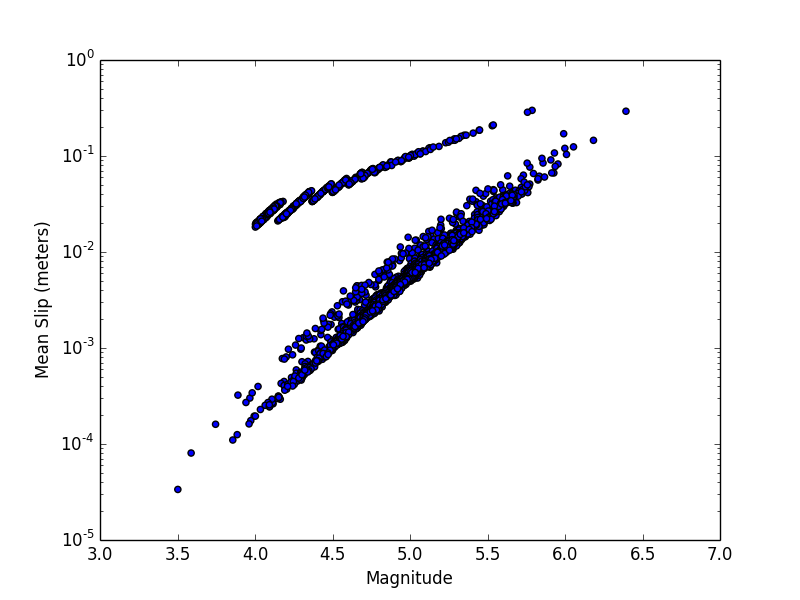
\includegraphics[width=0.49\textwidth]{graphics/mag_mean_slip_example.png}
\caption{\label{fig:mag_area_slip} \textbf{Left}: Example magnitude vs rupture area distribution.  \textbf{Right}: Example magnitude vs mean slip distribution. Compare these to Wells and Coppersmith 1994 relations.}
\end{figure}

\subsection{Earthquake Probability Plots}

To plot the conditional probabilities (Figure \ref{fig:probabilities}) of an earthquake with magnitude $\geq 7$ occurring on sections [4,5,6,7,8,9,10,11,12,13] (as defined in your fault model) as a function of time since the last earthquake on those sections:

\begin{verbatim}
$ python path/to/vq/pyvq/pyvq.py --event_file path/to/sim_file.h5 --event_file_type 
     'hdf5'  --plot_cond_prob_vs_t  --model_file path/to/model.txt --model_file_type
     'text' --min_magnitude 7.0 --use_sections 4 5 6 7 8 9 10 11 12 13
\end{verbatim}

To plot the expected waiting times until the next earthquake with magnitude $\geq 7$ occurring on sections [4,5,6,7,8,9,10,11,12,13] as a function of time since the last earthquake on those sections:

\begin{verbatim}
$ python path/to/vq/pyvq/pyvq.py --event_file path/to/sim_file.h5 --event_file_type 
     'hdf5'  --plot_waiting_times  --model_file path/to/model.txt --model_file_type
     'text' --min_magnitude 7.0 --use_sections 4 5 6 7 8 9 10 11 12 13
\end{verbatim}


\begin{figure}
\centering{}
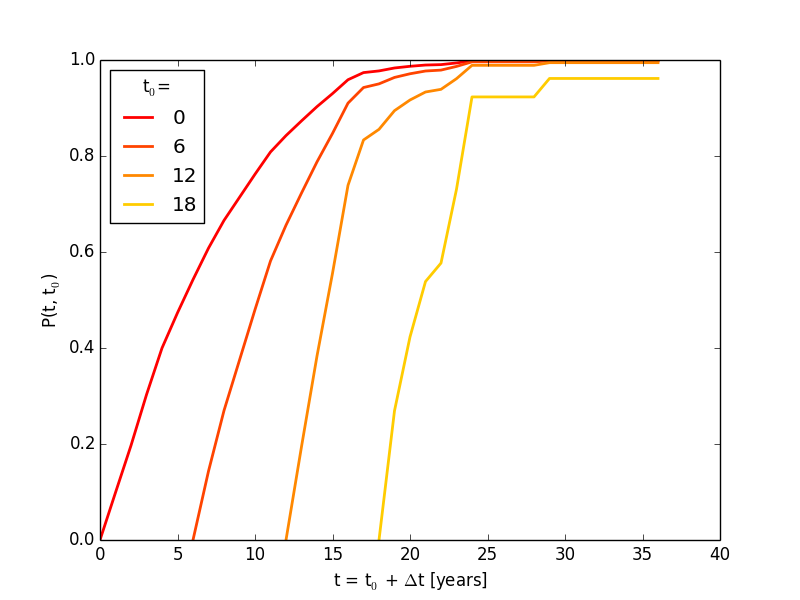
\includegraphics[width=0.49\textwidth]{graphics/cond_prob_vs_t_example.png}
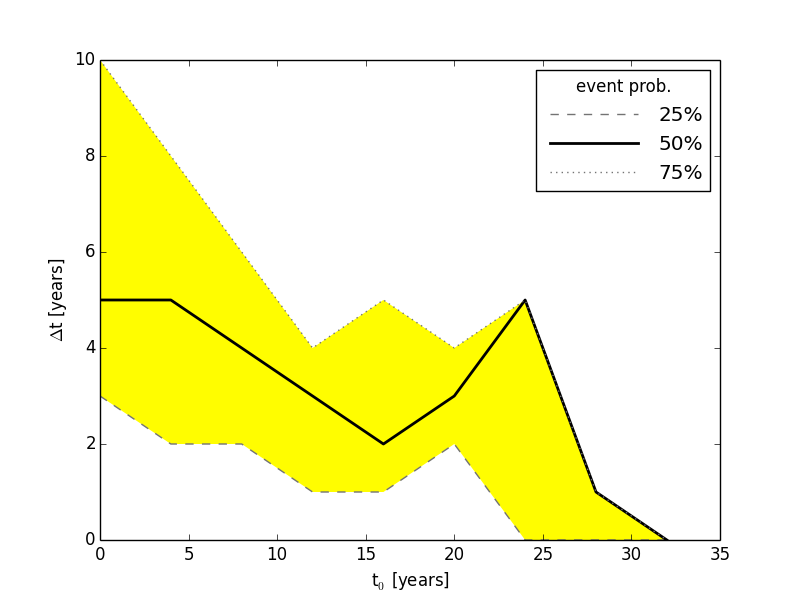
\includegraphics[width=0.49\textwidth]{graphics/waiting_times_example.png}
\caption{\label{fig:probabilities} \textbf{Left}: Conditional probability of an earthquake $M \geq 7$ on the specified sections as a function of time since the last earthquake $M \geq 7$. \textbf{Right}: Distribution of waiting times until the next earthquake $M \geq 7$ for waiting times with 25\%, 50\% and 75\% probability.}
\end{figure}


\subsection{Field Plots}

QuakeLib uses Green's functions to compute co-seismic fields given a fault geometry and a slip distribution. For displacements we use Okada's equations and for gravity, potential, and geoid height changes we use Okubo's equations. 

To compute the gravity changes for 5 meters of uniform slip on your fault model (example shown in Figure \ref{fig:single_element} for single 10km by 10km faults):

\begin{verbatim}
$ python path/to/vq/pyvq/pyvq.py --model_file path/to/model.txt --model_file_type
     'text' --uniform_slip 5 --field_plot --field_type 'gravity'
\end{verbatim}

\begin{figure}
\centering{}
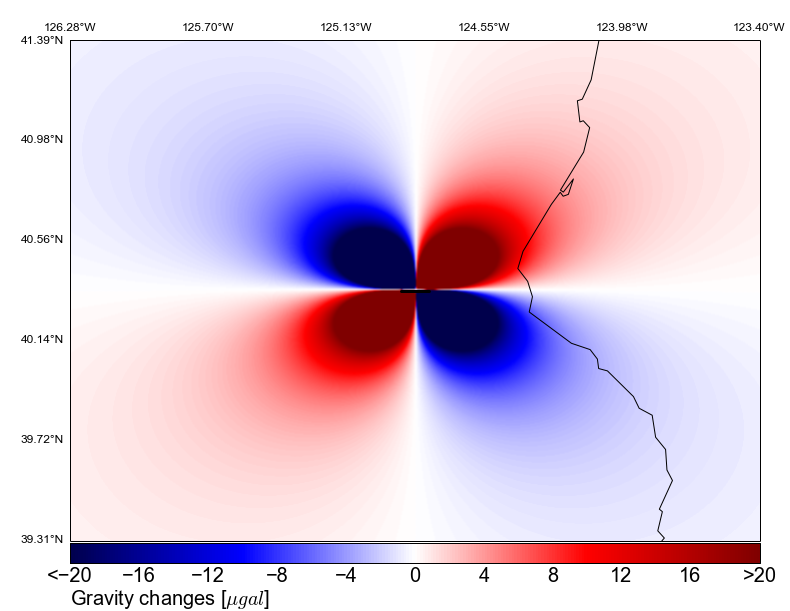
\includegraphics[width=0.49\textwidth]{graphics/example_vert_strikeslip_with_trace_fault_10000_gravity_uniform_slip5m.png}
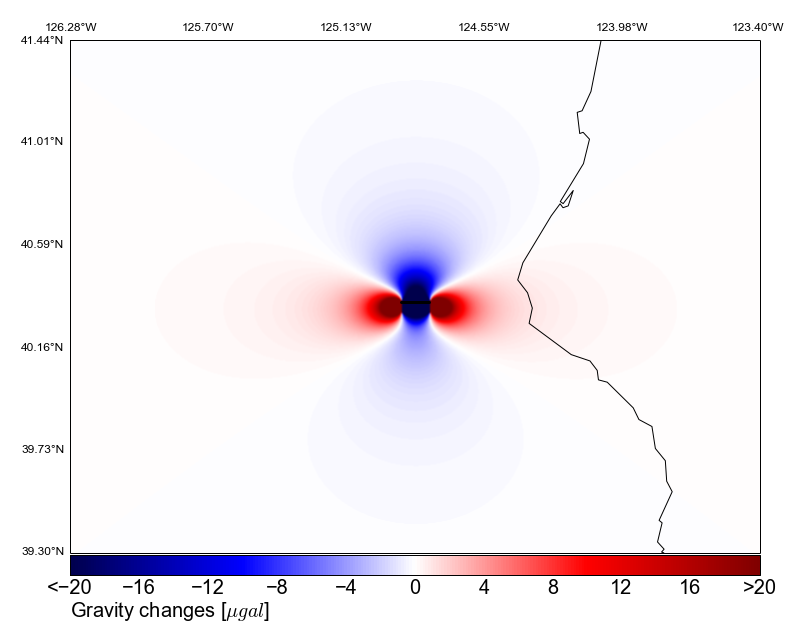
\includegraphics[width=0.48\textwidth]{graphics/example_normal_dip60_with_trace_fault_10000_gravity_uniform_slip1m.png}
\caption{\label{fig:single_element} \textbf{Left}: Gravity changes for 5m slip on a 10km by 10km vertical strikeslip fault. \textbf{Right}: Gravity changes for 1m slip on a 10km by 10km normal fault with dip angle 30 degrees.}
\end{figure}

To compute the gravity changes and InSAR interferogram for event \#210 from your simulation (Figures \ref{fig:event_insar} and \ref{fig:event_gravity}):

\begin{verbatim}
$ python path/to/vq/pyvq/pyvq.py --event_file path/to/sim_file.h5 --event_file_type 
     'hdf5' --model_file path/to/model.txt --model_file_type 'text' --field_plot 
     --field_type 'gravity' --event_id 210
     
$ python path/to/vq/pyvq/pyvq.py --event_file path/to/sim_file.h5 --event_file_type 
     'hdf5' --model_file path/to/model.txt --model_file_type 'text' --field_plot 
     --field_type 'insar' --event_id 210
\end{verbatim}


\begin{figure}
\centering
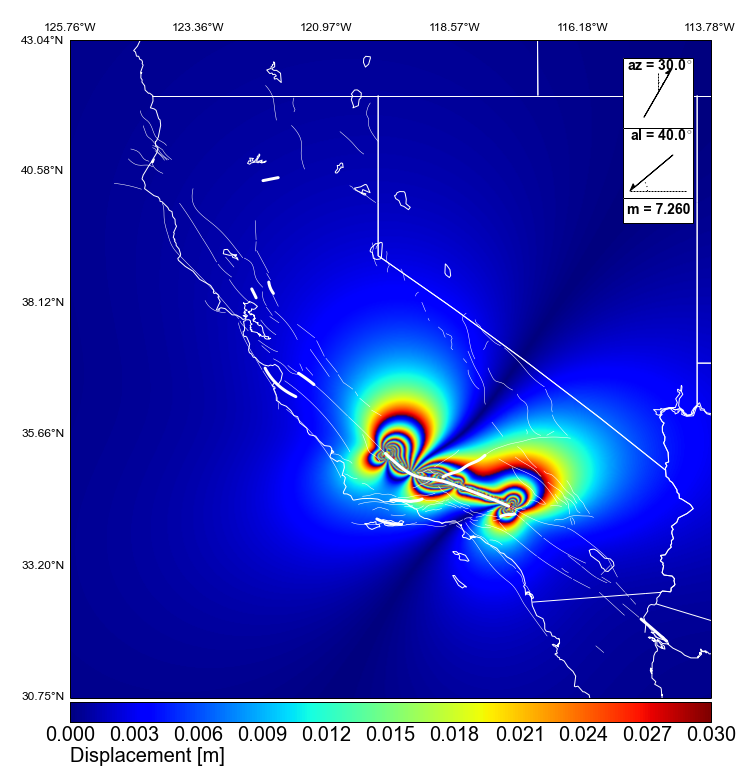
\includegraphics[width=\textwidth]{graphics/event_insar_example.png}
\caption{\label{fig:event_insar} Simulated InSAR interferogram for magnitude 7.26 earthquake on the San Andreas Fault. }
\end{figure}

\begin{figure}
\centering
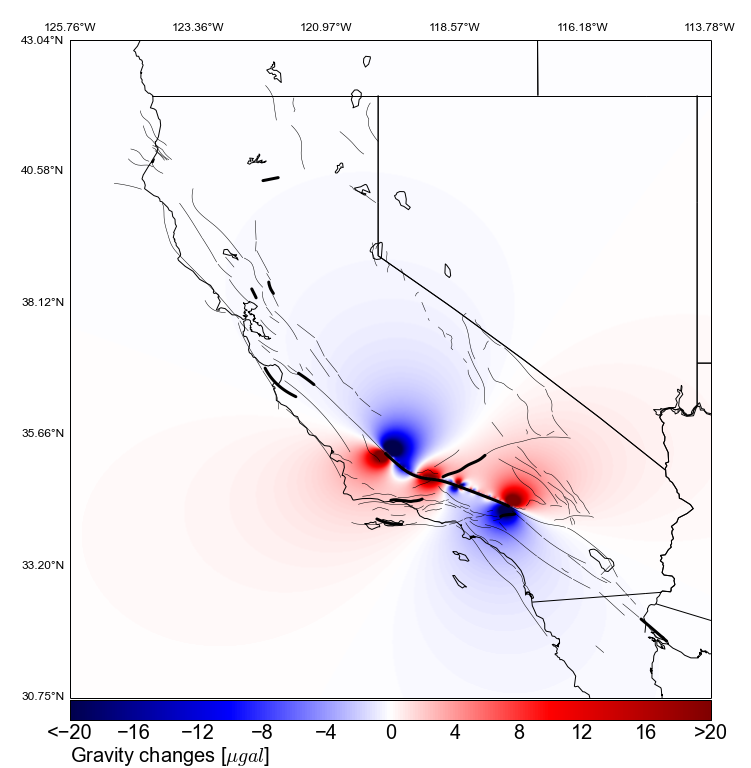
\includegraphics[width=\textwidth]{graphics/event_gravity_example.png}
\caption{\label{fig:event_gravity} Simulated gravity changes for magnitude 7.26 earthquake on the San Andreas Fault. }
\end{figure}

\section{PyVQ Plotting Arguments Grouped by Functionality\label{sec:pyvq_params}}

This section summarizes the current functionality of the pyvq script (section \ref{sec:pyvq}). These parameters do not have default values, and are not used unless specified. 

\subsection{Model parameters}

\noindent %
\begin{tabular}{|>{\raggedright}p{2in}|>{\raggedright}p{4.1in}|}
\hline 
\texttt{\small{--event\_file}} & The simulation output file.\tabularnewline
\hline 
\texttt{\small{--event\_file\_type}} & Either 'hdf5' or 'text'.\tabularnewline
\hline 
\texttt{\small{--sweep\_file}} & The simulation sweep file, required only if simulation file is text.\tabularnewline
\hline 
\texttt{\small{--model\_file}} & The fault model file.\tabularnewline
\hline 
\texttt{\small{--model\_file\_type}} & Either 'hdf5' or 'text'.\tabularnewline
\hline 
\end{tabular}

\subsection{Subsetting Parameters}
These parameters are used to select subsets of the faults or subsets of events. \\

\noindent %
\begin{tabular}{|>{\raggedright}p{2in}|>{\raggedright}p{4.1in}|}
\hline 
\texttt{\small{--use\_sections}} & Select a subset of the fault sections from the model file. To select sections 23, 43, and 101 it would be ``--use\_sections 23 43 101''.\tabularnewline
\hline 
\texttt{\small{--min\_magnitude}} & Select a minimum magnitude for earthquakes to be analyzed. To select earthquakes only above magnitude 5.5 it would be ``--min\_magnitude 5.5''.\tabularnewline
\hline 
\texttt{\small{--max\_magnitude}} & Select a maximum magnitude for earthquakes to be analyzed. Can be used in conjunction with --min\_magnitude to specify a range of magnitudes. \tabularnewline
\hline 
\end{tabular}


\subsection{\noindent Statistical Plotting Parameters}

\noindent %
\begin{tabular}{|>{\raggedright}p{2in}|>{\raggedright}p{4.1in}|}
\hline 
\texttt{\small{--plot\_freq\_mag n}} & Frequency-Magnitude. n=1 Normal plot, n=2 adds a Gutenberg-Richter line with b=1, n=3 adds UCERF2 observed seismicity rates in California, n=4 adds both the b=1 line and observed California rates.\tabularnewline
\hline 
\texttt{\small{--plot\_mag\_rupt\_area}} & Magnitude vs Rupture Area scaling. Compare to Wells and Coppersmith 1994.\tabularnewline
\hline 
\texttt{\small{--plot\_mag\_mean\_slip}} & Magnitude vs Mean Slip scaling. Compare to Wells and Coppersmith 1994.\tabularnewline
\hline
\texttt{\small{--all\_stat\_plots}} & Plot all statistical plots.\tabularnewline
\hline 
\texttt{\small{--wc94}} & Add Wells and Coppersmith 1994 scaling relation to Mean Slip or Rupture Area plots.\tabularnewline
\hline
\end{tabular}

\subsection{\noindent Probability Plotting Parameters}
These parameters can be used in combination with ``--use\_sections'', ``--min\_magnitude'', and ``--max\_magnitude'' to select subsets of your fault model and events for analysis. \\

\noindent %
\begin{tabular}{|>{\raggedright}p{2in}|>{\raggedright}p{4.1in}|}
\hline 
\texttt{\small{--plot\_prob\_vs\_t}} & Plot probability of earthquake as a function of time since the last earthquake.\tabularnewline
\hline 
\texttt{\small{--plot\_prob\_vs\_t\_fixed\_dt DT}} & Plot probability of earthquake in the next DT years as a function of time since the last earthquake. E.g. ``--plot\_prob\_vs\_t\_fixed\_dt 30'' plots the probability of an earthquake in the next 30 years as a function of time.\tabularnewline
\hline 
\texttt{\small{--plot\_cond\_prob\_vs\_t}} & Plot conditional probability of earthquake as a function of time since the last earthquake plotted at various times after the last earthquake to show the evolution of the distribution.\tabularnewline
\hline 
\texttt{\small{--plot\_waiting\_times}} & Plot the waiting times until the next earthquake as a function of time since the last earthquake, for waiting times with 25\%, 50\% and 75\% probability.\tabularnewline
\hline 
\texttt{\small{--beta}} & Beta parameter for the Weibull distribution, must also specify tau. If beta and tau are specified, the corresponding Weibull distribution is drawn in the ``--plot\_cond\_prob\_vs\_t'' plot.\tabularnewline
\hline 
\texttt{\small{--tau}} & Tau parameter for the Weibull distribution, must also specify beta.\tabularnewline
\hline 
\end{tabular}

\subsection{\noindent Field Plotting Parameters}
For any field plot you must specify ``--model\_file'' and ``--model\_file\_type''. To plot co-seismic fields, you must also specify an ``--event\_file'', ``--event\_file\_type'', and ``--event\_id''. To plot the field resulting from uniform slip across the entire fault model you must also specify ``--uniform\_slip''. \\

\noindent %
\begin{tabular}{|>{\raggedright}p{2in}|>{\raggedright}p{4.1in}|}
\hline 
\texttt{\small{--field\_plot}} & Required to plot any fields\tabularnewline
\hline 
\texttt{\small{--field\_type}} & The type of co-seismic field to plot. Options are: ``gravity'', ``dilat\_gravity'' (dilatational), ``displacement'', ``insar'', ``potential'' (gravitational potential), ``geoid'' (geoid height changes). \tabularnewline
\hline 
\texttt{\small{--event\_id}} & The number of the event to plot. \tabularnewline
\hline 
\texttt{\small{--uniform\_slip}} & The slip to apply to every fault element in the fault model, in meters.\tabularnewline
\hline
\texttt{\small{--colorbar\_max}} & The maximum value for the colorbar scale on field plots (excluding insar and displacement). E.g. to limit the gravity field plots to the color range -20 microGal to 20 microGal you would specify ``--colorbar\_max 20''. \tabularnewline
\hline 
\texttt{\small{--angles}} & The observing angles for displacements and InSAR, the field is projected along this direction. Must specify azimuth and elevation angles in degrees. E.g. ``--angles 20.5 66.2''. \tabularnewline
\hline 
\end{tabular}


%-------------------------------- End tutorials, begin appendices
\part{Appendices}

\appendix


\chapter{\label{cha:Appendix-A:-Input}Input Parameters for Virtual Quake}

\section{Input Parameters Grouped by Functionality}

This section explains the meaning of the input parameters for Virtual
Quake. These parameters are grouped by their functionality. Parameters
are given with their default values.


\subsection{Simulation time parameters}

\noindent %
\begin{tabular}{|>{\raggedright}p{2.3in}|>{\raggedright}p{3.8in}|}
\hline 
\texttt{\small{sim.time.start\_year = 0}} & The starting year of the simulation\tabularnewline
\hline 
\texttt{\small{sim.time.end\_year = 1000}} & The ending year of the simulation.\tabularnewline
\hline 
\end{tabular}


\subsection{\noindent System Parameters}

\noindent %
\begin{tabular}{|>{\raggedright}p{2.3in}|>{\raggedright}p{3.8in}|}
\hline 
\texttt{\small{sim.system.sanity\_check = false}} & Whether to perform sanity checks on simulation values each time step and abort if
any values are outside acceptable ranges.\tabularnewline
\hline 
\texttt{\small{sim.system.transpose\_matrix = true}} & Whether to store the Green's matrix in a transposed form to significantly
improve performance. This should only be set to false for comparative performance profiling.\tabularnewline
\hline 
\texttt{\small{sim.system.progress\_period = 0}} & How frequently (in wall time seconds) to display simulation progress. If
undefined or \textless{}= 0, simulation progress will not be displayed.\tabularnewline
\hline 
%\texttt{\small{sim.system.checkpoint\_period}} & How frequently (in simulation events) a checkpoint is saved. If undefined
%or \textless{}= 0, checkpoints will not be saved.\tabularnewline
%\hline 
%\texttt{\small{sim.system.checkpoint\_prefix = sim\_state\_}} & The prefix of the state save files, which will also include the event
%count.\tabularnewline
%\hline 
\end{tabular}


\subsection{Friction parameters}

\begin{tabular}{|>{\raggedright}p{2.3in}|>{\raggedright}p{3.8in}|}
\hline 
\texttt{\small{sim.friction.dynamic}} & The dynamic rupture value to use in the simulation from 0 to 1. Higher
values indicate ruptures are more likely to propagate along a fault
and result in larger earthquakes, while lower values indicate ruptures
are less likely to propagate and result in smaller earthquakes.\tabularnewline
\hline 
\end{tabular}


\subsection{Green's function parameters}

\begin{tabular}{|>{\raggedright}p{2.3in}|>{\raggedright}p{3.8in}|}
\hline 
\texttt{\small{sim.greens.method = standard}} & The method to calculate the Green's functions for fault element stress
interactions. There are three possible choices for this parameter
- \texttt{\small{standard}}, \texttt{\small{bh}} and \texttt{\small{file}}.
The \texttt{\small{standard}} option will calculate the Green's functions
using the normal Okada equations with all element-element interactions.
The \texttt{\small{bh}} option will use a Barnes Hut style approximation.
The \texttt{\small{file}} option will read precalculated values from
an input file (specified using \texttt{\small{sim.greens.input}}).\tabularnewline
\hline 
\texttt{\small{sim.greens.bh\_theta = 0.0}} & Parameter for Barnes Hut calculation of Green's function (between
0 and 1). Lower values mean less of an approximation. If undefined,
defaults to 0 (meaning it effectively doesn't use Barnes Hut approximation).\tabularnewline
\hline 
\texttt{\small{sim.greens.input}} & If \texttt{\small{sim.greens.method}} is defined as \texttt{\small{file}},
this is the name of the HDF5 file to read the Green's function values
from.\tabularnewline
\hline 
\texttt{\small{sim.greens.output}} & The name of the HDF5 file to write the Green's function values to. If unspecified, Green's function values are not written to a file after being calculated.\tabularnewline
\hline 
\texttt{\small{sim.greens.use\_normal = true}} & Whether to use the Green's normal stress function in calculations
or just the Green's shear function.\tabularnewline
\hline 
\texttt{\small{sim.greens.kill\_distance = 0.0}} & Kills interaction between any two elements greater than this distance
(in km) apart. If undefined or \textless{}= 0, all interactions will
remain the same.\tabularnewline
\hline 
\texttt{\small{sim.greens.sample\_distance = 1000.0}} & When calculating the Green's function, take samples at this minimum distance between samples.  This allows better convergence between models with few large elements and models with many small elements.  If the element size is smaller than this value, it has no effect.\tabularnewline
\hline 
\end{tabular}


\subsection{File name parameters}

\begin{tabular}{|>{\raggedright}p{2.3in}|>{\raggedright}p{3.8in}|}
\hline 
\texttt{\small{sim.file.input}} & The input model file of the simulation.\tabularnewline
\hline 
\texttt{\small{sim.file.input\_type}} & The input model file format - must be one of text or hdf5.\tabularnewline
\hline 
\texttt{\small{sim.file.output\_event}} & The file which events will be written to. If undefined, events will
not be recorded.\tabularnewline
\hline 
\texttt{\small{sim.file.output\_sweep}} & The file which sweeps will be written to. If undefined, sweeps will
not be recorded.\tabularnewline
\hline 
\texttt{\small{sim.file.output\_event\_type}} & The file format to output events - must be one of text or hdf5.  If hdf5, sweep and event information will be printed to the same file specified by \texttt{sim.file.output\_event}.\tabularnewline
\hline 
\end{tabular}


%\subsection{EqSim File Parameters}
%
%\begin{tabular}{|>{\raggedright}p{2.3in}|>{\raggedright}p{3.8in}|}
%\hline 
%\texttt{\small{sim.eqsim.file.output}} & The file which EqSim style event logging will be written to. If undefined,
%the EqSim events file will not be created.\tabularnewline
%\hline 
%\texttt{\small{sim.eqsim.file.condition}} & The file to read EqSim style initial condition information from. If
%undefined, initial shear and normal stresses will be 0 and rhogd will
%be 1.557e8.\tabularnewline
%\hline 
%\texttt{\small{sim.eqsim.file.friction}} & The file to read EqSim style friction information from. If undefined,
%EqSim input files will not be used.\tabularnewline
%\hline 
%\texttt{\small{sim.eqsim.file.geometry}} & The file to read EqSim style geometry information from. If undefined,
%EqSim input files will not be used.\tabularnewline
%\hline 
%\texttt{\small{sim.eqsim.file.slipmap\_mag = 7.5}} & The magnitude cutoff to print slip maps in the EqSim event file.\tabularnewline
%\hline 
%\end{tabular}


\subsection{BASS (Branching Aftershock Sequence) model parameters}

\begin{tabular}{|>{\raggedright}p{2.3in}|>{\raggedright}p{3.8in}|}
\hline 
\texttt{\small{sim.bass.max\_generations = 0}} & Maximum number of aftershock generations to generate in BASS model.
If this is 0 then the BASS aftershock model will not be used.\tabularnewline
\hline 


\texttt{\small{sim.bass.mm = 4.0}}{\small \par}

\texttt{\small{sim.bass.dm = 1.25}}{\small \par}

\texttt{\small{sim.bass.b = 1.0}}{\small \par}

\texttt{\small{sim.bass.c = 0.1}}{\small \par}

\texttt{\small{sim.bass.p = 1.25}}{\small \par}

\texttt{\small{sim.bass.d = 300}}{\small \par}

\texttt{\small{sim.bass.q = 1.35}} & Different parameters for BASS model. See paper \cite{Turcotte:2007up}
for details.

Mm: minimum magnitude

dM: strength of aftershock sequence (intensity of aftershocks)

b: scaling of frequency magnitude

c: start of aftershocks in days

p: time decay rate of aftershocks

d: distance parameter for aftershocks in meters

q: distance decay rate\tabularnewline
\hline 
\end{tabular}


%\subsection{Parallel simulation parameters}
%
%\noindent %
%\begin{tabular}{|>{\raggedright}p{2.3in}|>{\raggedright}p{3.8in}|}
%\hline 
%\texttt{\small{sim.parallel.spec\_exec = none}} & Choose the type of speculative execution to be used to improve simulation
%speed. Currently experimental. Can be either \texttt{\small{none}},
%\texttt{\small{fixed}}, or \texttt{\small{adaptive}}. If \texttt{none}
%is chosen, speculative execution will not be used. If \texttt{\small{fixed}}
%or \texttt{\small{adaptive}} are chosen, the speculative execution
%scheme is used with either a fixed boundary distance or adaptive distance.\tabularnewline
%\hline 
%\texttt{sim.parallel.spec\_exec\_distance = 0} & The boundary distance to use in the \texttt{\small{fixed}} speculative
%execution scheme. This affects how frequently the simulation goes
%into speculative mode.\tabularnewline
%\hline 
%\end{tabular}
%

\chapter{Virtual Quake Input Model Format}



\section{\label{sec:Trace-File-Format}Trace File Format}

The initial fault geometry for VQ runs is defined by the trace file.
Each trace file describes a single fault by the location of points
along the fault trace and associated fault characteristics at each
of the points. A single VQ model for a simulation can be generated
by combining multiple fault traces using the mesher program (see Section
\ref{sec:Tutorial_multiple} for an example).

The trace files are ASCII format with comments indicated by a \# (hash)
mark. Lines that begin with a \# will be ignored and any values after
a \# in a line will be ignored. The initial line in the trace file
outlines the fault described in the file using the following attributes:\vspace*{\bigskipamount}


\noindent %
\begin{tabular}{|>{\raggedright}p{1.85in}|>{\raggedright}p{4.25in}|}
\hline 
\texttt{fault\_id} & ID number of the parent fault of this section. Used to unify multi-segment
faults defined in separate files.\tabularnewline
\hline 
\texttt{num\_points} & The number of trace points comprising this section.\tabularnewline
\hline 
\texttt{section\_name} & Name of the section, may not contain whitespace.\tabularnewline
\hline 
\end{tabular}

\vspace*{\bigskipamount}
The remainder of the file defines each of the trace points for the
fault. Each trace point is described using the following attributes.
The units of the attributes in the file were chosen to be easily human
understandable. In the simulation they are converted to SI
units though this is hidden from the user.\vspace*{\bigskipamount}


\noindent %
\begin{tabular}{|>{\raggedright}p{1.85in}|>{\raggedright}p{4.25in}|}
\hline 
\texttt{latitude} & Latitude of trace point (must be in {[}-90, 90{]}).\tabularnewline
\hline 
\texttt{longitude} & Longitude of trace point (must be in {[}-180, 180{]}).\tabularnewline
\hline 
\texttt{altitude} & Altitude of trace point in meters above ground. All faults should
be underground (negative altitude). Faults defined above ground will
have undefined results.\tabularnewline
\hline 
\texttt{depth\_along\_dip} & The depth of the fault along the dip in meters (must be greater than
0). For a dip angle of $\delta$ the actual depth of the fault will
be depth\_along\_dip{*}$\sin \delta$.\tabularnewline
\hline 
\texttt{slip\_rate} & The long term slip rate of the fault in centimeters per year.\tabularnewline
\hline 
\texttt{aseismic} & The fraction of slip that is aseismic (must be in {[}0,1{]}).\tabularnewline
\hline 
\texttt{rake} & The fault rake angle in degrees (must be in {[}-180, 180{]}).\tabularnewline
\hline 
\texttt{dip} & The fault dip angle in degrees (must be in {[}0,90{]}).\tabularnewline
\hline 
\texttt{lame\_mu} & Lame's mu parameter describing material properties in Pascals (must
be greater than 0).\tabularnewline
\hline 
\texttt{lame\_lambda} & Lame's lambda parameter describing material properties in Pascals.\tabularnewline
\hline 
\end{tabular}


\chapter{\label{cha:Appendix-C:Mesher_Parameters}Mesher Program Options}


\section{Mesher Options Grouped by Functionality}

This section explains the meaning of the options used by the mesher
program for Virtual Quake model file manipulation. These options
are grouped by their functionality. 


\subsection{General Options}

\noindent %
\begin{tabular}{|>{\raggedright}p{3.05in}|>{\raggedright}p{3.05in}|}
\hline 
-s FILE, -\/-print\_statistics=FILE & Print statistics regarding final model to the specified file.\tabularnewline
\hline 
-m, -\/-merge\_duplicate\_verts & Merge duplicate vertices after importing files.\tabularnewline
\hline 
-d, -\/-delete\_unused & Delete unused vertices after importing files.\tabularnewline
\hline 
\end{tabular}


\subsection{\noindent File Import Options}

\noindent %
\begin{tabular}{|>{\raggedright}p{3.05in}|>{\raggedright}p{3.05in}|}
\hline 
-i FILE, -\/-import\_file=FILE & Specify a model file to import and merge. Must have a paired import\_file\_type.\tabularnewline
\hline 
-j TYPE, -\/-import\_file\_type=TYPE & Specify a model file type for importing. Must have a paired import\_file.\tabularnewline
\hline 
-l FILE, -\/-import\_trace\_element\_size=FILE & Specify the element size to use for trace file meshing. Must have
a paired trace type file import.\tabularnewline
\hline 
-t METHOD, -\/-taper\_fault\_method=METHOD & Specify the how to taper the imported trace when meshing. Must have
a paired trace type file import. Choices for taper method are: none,
taper, taper\_full, taper\_renorm. %Taper follows the convention of \ref{sec:tapering}.
\tabularnewline
\hline 
-C FILE, -\/-import\_eqsim\_condition=FILE & Specify an EQSim condition file to import for the model.\tabularnewline
\hline 
-F FILE, -\/-import\_eqsim\_friction=FILE & Specify an EQSim friction file to import for the model.\tabularnewline
\hline 
-G FILE, -\/-import\_eqsim\_geometry=FILE & Specify an EQSim geometry file to import for the model.\tabularnewline
\hline 
\end{tabular}


\subsection{\noindent File Export Options}

\noindent %
\begin{tabular}{|>{\raggedright}p{3.05in}|>{\raggedright}p{3.05in}|}
\hline 
-e FILE, -\/-export\_file=FILE & Specify a file to export the completed model to. Must have a paired
export\_file\_type.\tabularnewline
\hline 
-f TYPE, -\/-export\_file\_type=TYPE & Specify a file type to export the completed model. Must have a paired
export\_file.\tabularnewline
\hline 
-D FILE, -\/-export\_eqsim\_condition=FILE & Specify an EQSim condition file to export for the model.\tabularnewline
\hline 
-R FILE, -\/-export\_eqsim\_friction=FILE & Specify an EQSim friction file to export for the model.\tabularnewline
\hline 
-M FILE, -\/-export\_eqsim\_geometry=FILE & Specify an EQSim geometry file to export for the model.\tabularnewline
\hline 
\end{tabular}


\chapter{\label{chap:Virtual-Quake-Output}Virtual Quake Output
File Format}


\section{Introduction}

The format of the output files of Virtual Quake is described
here. All outputs are in non-dimensional units unless otherwise specified.


\section{HDF5 Output}

If Virtual Quake is compiled with the HDF5 library it is possible
to output simulation results in this format. The output file is composed of several tables
and datasets describing the input and output to a simulation. Depending
on user options some of these tables may be empty but they will always
exist in the file.

\subsection{About HDF5}

The Hierarchical Data Format (HDF) is a portable file format developed
at the National Center for Supercomputing Applications (NCSA) \url{hdf.ncsa.uiuc.edu/HDF5}.
It is designed for storing, retrieving, analyzing, visualizing, and
converting scientific data. The current and most popular version is
HDF5, which stores multi-dimensional arrays together with ancillary
data in a portable self-describing format. 

HDF5 files are organized in a hierarchical structure, similar to a
Unix file system. Two types of primary objects, \textit{groups} and
\textit{datasets}, are stored in this structure. A group contains
instances of zero or more groups or datasets, while a dataset stores
a multi-dimensional array of data elements. Both kinds of objects
are accompanied by supporting metadata.

A dataset is physically stored in two parts: a header and a data array.
The header contains miscellaneous metadata describing the dataset
as well as information that is needed to interpret the array portion
of the dataset. Essentially, it includes the name, datatype, dataspace,
and storage layout of the dataset. The name is a text string identifying
the dataset. The datatype describes the type of the data array elements.
The dataspace defines the dimensionality of the dataset, i.e., the
size and shape of the multi-dimensional array. The dimensions of a
dataset can be either fixed or unlimited (extensible). The storage
layout specifies how the data arrays are arranged in the file.


\subsubsection{Accessing Data Using HDFView}

NCSA HDFView is a visual tool for accessing HDF files. You can use
it for viewing the internal file hierarchy in a tree structure, creating
new files, adding or deleting groups and datasets, and modifying existing
datasets. HDFView is capable of displaying 2D slices of multi-dimensional
datasets, with navigation arrow buttons that enable you to range over
the entire extent of a third dimension.


%\subsection{Element Table}
%
%The table titled \texttt{\small{block\_info\_table}} describes the
%set of all elements used in the simulation. The information for each
%element is a row in the table, with each column representing an attribute
%of the block. The attributes are defined as follows:\vspace*{\bigskipamount}
%
%
%\begin{tabular}{|>{\raggedright}p{1.5in}|>{\raggedright}p{4.25in}|}
%\hline 
%Attribute Name & Attribute Description\tabularnewline
%\hline 
%\hline 
%\texttt{\small{block\_id}} & A numerical ID of the element. These IDs should be in contiguousascending
%numerical order.\tabularnewline
%\hline 
%\texttt{\small{fault\_id}} & A numerical ID for the fault the element belongs to. This allows elements
%to be grouped by fault.\tabularnewline
%\hline 
%\texttt{\small{section\_id}} & A numerical ID for the subsection of the fault the element belongs
%to (if any). This allows faults to be subdivided into geologically
%distinct zones.\tabularnewline
%\hline 
%\texttt{\small{m\_x\_pt1}} & The X coordinate of the 1st point defining the element (in meters).\tabularnewline
%\hline 
%\texttt{\small{m\_y\_pt1}} & The Y coordinate of the 1st point defining the element (in meters).\tabularnewline
%\hline 
%\texttt{\small{m\_z\_pt1}} & The Z coordinate of the 1st point defining the element (in meters).\tabularnewline
%\hline 
%\texttt{\small{m\_das\_pt1}} & The distance of the 1st point along the fault strike (in meters).\tabularnewline
%\hline 
%\texttt{\small{m\_trace\_flag\_pt1}} & EqSim specific flag defining where the 1st point is on the fault trace.\tabularnewline
%\hline 
%\texttt{\small{m\_x\_pt2}} & The X coordinate of the 2nd point defining the element (in meters).\tabularnewline
%\hline 
%\texttt{\small{m\_y\_pt2}} & The Y coordinate of the 2nd point defining the element (in meters).\tabularnewline
%\hline 
%\texttt{\small{m\_z\_pt2}} & The Z coordinate of the 2nd point defining the element (in meters).\tabularnewline
%\hline 
%\texttt{\small{m\_das\_pt2}} & The distance of the 2nd point along the fault strike (in meters).\tabularnewline
%\hline 
%\texttt{\small{m\_trace\_flag\_pt2}} & EqSim specific flag defining where the 2nd point is on the fault trace.\tabularnewline
%\hline 
%\texttt{\small{m\_x\_pt3}} & The X coordinate of the 3rd point defining the element (in meters).\tabularnewline
%\hline 
%\texttt{\small{m\_y\_pt3}} & The Y coordinate of the 3rd point defining the element (in meters).\tabularnewline
%\hline 
%\texttt{\small{m\_z\_pt3}} & The Z coordinate of the 3rd point defining the element (in meters).\tabularnewline
%\hline 
%\texttt{\small{m\_das\_pt3}} & The distance of the 3rd point along the fault strike (in meters).\tabularnewline
%\hline 
%\texttt{\small{m\_trace\_flag\_pt3}} & EqSim specific flag defining where the 3rd point is on the fault trace.\tabularnewline
%\hline 
%\texttt{\small{m\_x\_pt4}} & The X coordinate of the 4th point defining the element (in meters).\tabularnewline
%\hline 
%\texttt{\small{m\_y\_pt4}} & The Y coordinate of the 4th point defining the element (in meters).\tabularnewline
%\hline 
%\texttt{\small{m\_z\_pt4}} & The Z coordinate of the 4th point defining the element (in meters).\tabularnewline
%\hline 
%\texttt{\small{m\_das\_pt4}} & The distance of the 4th point along the fault strike (in meters).\tabularnewline
%\hline 
%\texttt{\small{m\_trace\_flag\_pt4}} & EqSim specific flag defining where the 4th point is on the fault trace.\tabularnewline
%\hline 
%\texttt{\small{slip\_velocity}} & The long term slip velocity of the element (in meters/second).\tabularnewline
%\hline 
%\texttt{\small{aseismicity}} & The fraction of the element slip that is aseismic (from 0 to 1).\tabularnewline
%\hline 
%\texttt{\small{rake\_rad}} & The rake angle of the element (in radians).\tabularnewline
%\hline 
%\texttt{\small{dip\_rad}} & The dip angle of the element (in radians).\tabularnewline
%\hline 
%\texttt{\small{dynamic\_strength}} & The dynamic strength of the element (in Pascals).\tabularnewline
%\hline 
%\texttt{\small{static\_strength}} & The static strength of the element (in Pascals).\tabularnewline
%\hline 
%\texttt{\small{lame\_mu}} & The Lam� mu parameter used to calculate Green's function values on
%the element (in Pascals).\tabularnewline
%\hline 
%\texttt{\small{lame\_lambda}} & The Lam� lambda parameter used to calculate Green's function values
%on the element (in Pascals).\tabularnewline
%\hline 
%\texttt{\small{fault\_name}} & The name of the fault associated with the element.\tabularnewline
%\hline 
%\end{tabular}


\section{Events}

The table titled \texttt{\small{event\_table}} describes the events
that occurred during a simulation. This table gives a more general
overview of the event information, with detailed information (e.g.
which blocks slipped by how much in what order releasing how much
stress) given in \texttt{\small{event\_sweep\_table}}. Corresponding data is instead written to ASCII text files if the appropriate parameter is set in the simulation parameter file.  \vspace*{\bigskipamount}


\begin{tabular}{|>{\raggedright}p{1.5in}|>{\raggedright}p{4.25in}|}
\hline 
Attribute Name & Attribute Description\tabularnewline
\hline 
\hline 
\texttt{\small{event\_number}} & A unique numerically ascending ID number of the event.\tabularnewline
\hline 
\texttt{\small{event\_year}} & The simulation year that the event occurred in.\tabularnewline
\hline 
\texttt{\small{event\_trigger}} & The ID of the block that triggered the event, i.e. the ID of the first
block to fail.\tabularnewline
\hline 
\texttt{\small{event\_magnitude}} & The moment magnitude of the event calculated based on the area, slip
and shear modulus.\tabularnewline
\hline 
\texttt{\small{event\_shear\_init}} & The summed initial shear stress on all blocks involved in the event
(in Pascals).\tabularnewline
\hline 
\texttt{\small{event\_normal\_init}} & The summed initial normal stress on all blocks involved in the event
(in Pascals).\tabularnewline
\hline 
\texttt{\small{event\_shear\_final}} & The summed final shear stress on all blocks involved in the event
(in Pascals).\tabularnewline
\hline 
\texttt{\small{event\_normal\_final}} & The summed final normal stress on all blocks involved in the event
(in Pascals).\tabularnewline
\hline 
\texttt{\small{start\_sweep}} & The ID of the first sweep of the event.\tabularnewline
\hline 
\texttt{\small{end\_sweep}} & The ID of the final sweep of the event.\tabularnewline
\hline 
\end{tabular}


\section{Event Sweeps}

The table titled \texttt{\small{event\_sweep\_table}} describes the
individual block failures in the sweeps during an event. There can
be multiple sweeps within an event and there can be multiple block
failures within each sweep. Each line in the table represents a block
failure in a given sweep. Corresponding data is instead written to ASCII text files if the appropriate parameter is set in the simulation parameter file. \vspace*{\bigskipamount}


\begin{tabular}{|>{\raggedright}p{1.5in}|>{\raggedright}p{4.25in}|}
\hline 
Attribute Name & Attribute Description\tabularnewline
\hline 
\hline 
\texttt{\small{event\_number}} & The event which this sweep is a part of.\tabularnewline
\hline 
\texttt{\small{sweep\_num}} & The numerical ID of the sweep within the event (starts at 0 for each
event).\tabularnewline
\hline 
\texttt{\small{block\_id}} & The numerical ID of the block that failed.\tabularnewline
\hline 
\texttt{\small{slip}} & The amount that the block slipped in this sweep, not cumulative (in
meters).\tabularnewline
\hline 
\texttt{\small{area}} & The area of the block that slipped (in square meters)\tabularnewline
\hline 
\texttt{\small{mu}} & The shear modulus of the block (in Pascals).\tabularnewline
\hline 
\texttt{\small{shear\_init}} & The shear stress on the block before the sweep (in Pascals).\tabularnewline
\hline 
\texttt{\small{normal\_init}} & The normal stress on the block before the sweep (in Pascals).\tabularnewline
\hline 
\texttt{\small{shear\_final}} & The shear stress on the block at the end of the sweep (in Pascals).\tabularnewline
\hline 
\texttt{\small{normal\_final}} & The normal stress on the block at the end of the sweep (in Pascals).\tabularnewline
\hline 
\end{tabular}


\chapter{\label{chap:License}License }

Copyright (c) 2012-2014 Eric M. Heien, Michael K. Sachs, Kasey W. Schultz, John B. Rundle

Permission is hereby granted, free of charge, to any person obtaining
a copy of this software and associated documentation files (the ``Software''),
to deal in the Software without restriction, including without limitation
the rights to use, copy, modify, merge, publish, distribute, sublicense,
and/or sell copies of the Software, and to permit persons to whom
the Software is furnished to do so, subject to the following conditions:

The above copyright notice and this permission notice shall be included
in all copies or substantial portions of the Software.

THE SOFTWARE IS PROVIDED ``AS IS'', WITHOUT WARRANTY
OF ANY KIND, EXPRESS OR IMPLIED, INCLUDING BUT NOT LIMITED TO THE
WARRANTIES OF MERCHANTABILITY, FITNESS FOR A PARTICULAR PURPOSE AND
NONINFRINGEMENT. IN NO EVENT SHALL THE AUTHORS OR COPYRIGHT HOLDERS
BE LIABLE FOR ANY CLAIM, DAMAGES OR OTHER LIABILITY, WHETHER IN AN
ACTION OF CONTRACT, TORT OR OTHERWISE, ARISING FROM, OUT OF OR IN
CONNECTION WITH THE SOFTWARE OR THE USE OR OTHER DEALINGS IN THE SOFTWARE.\bibliographystyle{plain}
\bibliography{vq}

\end{document}
%%%%%%%%%%%%%%%%%%%%%%%%%%%%%%%%%%% END VQ manual from Lyx code
